\documentclass[preprint, 12pt]{elsarticle}
\usepackage[utf8]{inputenc}
\usepackage{color}
\usepackage{graphicx}
\usepackage{placeins}
\usepackage[margin=1in]{geometry}
\usepackage{appendix}
\usepackage{amsmath, amssymb, bm}
\usepackage{multirow}
\usepackage{placeins}
\usepackage{xfrac}
\usepackage[colorlinks=true, linkcolor=blue, citecolor=blue]{hyperref}
\usepackage[nameinlink, capitalize]{cleveref}
\usepackage[font=footnotesize, labelfont=bf]{caption}
\usepackage{subcaption}
\usepackage[version=4]{mhchem}
\usepackage{lineno}
\usepackage{bm}
\usepackage{comment}
\usepackage[T1]{fontenc}
%\usepackage{newtxtext,newtxmath}

\journal{Journal of Nuclear Materials}

\begin{document}

\begin{frontmatter}

\title{Assessment of uranium nitride interatomic potentials}

\author[ncsu]{Mohamed AbdulHameed}
\author[ncsu,inl]{Benjamin Beeler\corref{qwe}}
\cortext[qwe]{Corresponding author}
\ead{bwbeeler@ncsu.edu}
\author[lanl]{Conor O.T. Galvin}
\author[lanl]{Michael W.D. Cooper}

\address[ncsu]{Department of Nuclear Engineering, North Carolina State University, Raleigh, NC 27695}
\address[inl]{Idaho National Laboratory, Idaho Falls, ID 83415}
\address[lanl]{Los Alamos National Laboratory, Los Alamos, NM 87545}

\begin{abstract}

Uranium mononitride (UN) is a promising nuclear fuel due to its high fissile density, high thermal conductivity, and suitability for reprocessing. In this study, two uranium nitride interatomic potentials are assessed: Tseplyaev and Starikov's angular-dependent potential and Kocevski \textit{et al.}'s embedded atom model potential. Predictions of the thermophysical and elastic properties of UN, \ce{UN2}, and $\alpha$- and $\beta$-\ce{U2N3} computed using both potentials are assessed and compared to available experimental data. The Tseplyaev potential performs better with the energetic aspects of UN, e.g., specific heat capacity and point defect formation energies, whereas the Kocevski potential performs better with the structural aspects of UN, e.g., thermal expansion as well as with the elastic properties. The reasons why the Kocevski potential underestimates the UN specific heat are explained by examining the UN phonon properties modeled using both potentials. The Kocevski potential shows better identification of the mechanical stability ranges of UN, \ce{UN2}, and $\alpha$- and $\beta$-\ce{U2N3}, reasonably predicting the melting point of UN and predicting stable structures for \ce{UN2} and $\alpha$- and $\beta$-\ce{U2N3}. On the other hand, the Tseplyaev potential predicts a premature phase change of both UN and \ce{UN2} and cannot stabilize $\alpha$- nor $\beta$-\ce{U2N3}. However, the Kocevski potential cannot predict a stable $\alpha$-U phase and is thus not suitable for the calculation of formation energies for non-stoichiometric point defects.

\end{abstract}

\begin{keyword}
uranium nitride \sep thermophysical properties \sep molecular dynamics \sep phonons \sep point defects
\end{keyword}

\end{frontmatter}

\linenumbers

\section{Introduction}

Since the 2011 Fukushima Daiichi accident in Japan, research efforts have been directed to develop advanced nuclear fuels that have improved performance in extreme conditions compared to \ce{UO2} while maintaining thermodynamic and mechanical stability \cite{Watkins2021}. One such fuel candidate is uranium mononitride (UN), which has shown many positive characteristics including high fissile density, high thermal conductivity, good dissolution in nitric acid making it compatible with the PUREX process, good chemical compatibility with most potential cladding materials, and longer fuel residence time \cite{Ekberg2018, Wallenius2020, Uno2020}. However, it has also suffered some drawbacks that historically hindered its industrial adoption, including complicated fabrication processes, high fuel cost owing to the need for N-15 enrichment, low resistance to oxidation by high-temperature steam, and high swelling rates \cite{Ekberg2018, Wallenius2020, Uno2020}.

UN has not been investigated as widely as oxide fuels, and many aspects of its behavior at high temperatures and under irradiation are not well understood \cite{Casagranda2020}. To address its drawbacks and build a case for its practical use in light-water and advanced reactors, UN properties should be well-understood at the atomic and mesoscales. Multiscale multiphysics fuel performance models can provide a pathway for the descriptive and predictive evolution of nuclear fuels and are especially valuable in cases where experimental data is limited. These models, however, require many input parameters from lower-length scale simulation methods like density functional theory (DFT) and molecular dynamics (MD).

Many DFT studies have been conducted on UN to predict its electronic structure and magnetic ordering \cite{Samsel2007, Evarestov2008, Gryaznov2012, Mei2013, Kocevski2022I} as well as to understand the properties of its point defects \cite{Kotomin2007, Kotomin2009, Bocharov2011, Lan2013}, impurities \cite{Kotomin2008}, and fission products \cite{Klipfel2012, Claisse2016, Zhang2015, Yang2021}. However, DFT is computationally demanding and has limitations in system size and simulation time. MD simulations can overcome these limitations and offer more flexibility in predicting fuel behavior at finite temperatures. Still, the accuracy of MD results is highly dependent on the quality of the interatomic potentials employed. Therefore, a reliable UN interatomic potential is a necessity.

For UN, several interatomic potentials exist in the literature. Kurosaki \textit{et al.} \cite{Kurosaki2000I, Kurosaki2000II} developed a Busing-Ida type potential which they used to predict thermal expansion, constant-pressure specific heat capacity, and thermal conductivity. Calculated properties qualitatively agree with experimental results at low temperatures and exhibit an increasing underestimation with increasing temperature. Kurosaki \textit{et al.} mention the values of potential parameters without units, which makes it hard to further assess its behavior. Chen \textit{et al.} \cite{Chen2010} used the Chen–Möbius lattice inversion method to derive three Morse-type pair potentials for the U-U, N-N, and U-N interactions. The potential was then used to predict thermal expansion and compressibility with a moderate qualitative agreement. However, Morse-type potentials cannot capture the nature of atomic bonding, especially in covalent solids such as UN \cite{Mishin2005}.

Kuksin \textit{et al.} \cite{Kuksin2016} developed an angular-dependent potential (ADP) fitted to DFT calculations. The potential was modified in a later paper by Tseplyaev and Starikov \cite{Tseplyaev2016}, and used to calculate point defect formation and migration energies and to predict the UN pressure-induced $Fm\Bar{3}m \rightarrow R\Bar{3}m$ phase transition. However, the authors didn't consider the effect of stoichiometry on defect formation energies, and their methodology to calculate the U and N chemical potentials is not reported. They also show evidence of the potential's capability to predict some basic properties of \ce{UN2} and \ce{U2N3}. Li and Murphy \cite{Li2021} have later used this potential to study self-diffusion in hypo-stoichiometric UN.

Kocevski \textit{et al.} \cite{Kocevski2022II} developed an embedded-atom method (EAM) potential fitted to experimental thermal expansion and single crystal elastic constants, as well as formation energies of stoichiometric point defects from DFT calculations. The potential reproduced observed elastic properties and temperature-dependent heat capacity with reasonable agreement and was also used to study Xe diffusion in UN.

Tseplyaev and Starikov's ADP (hereafter referred to as the Tseplyaev potential) and Kocevski \textit{et al.}'s EAM potential (hereafter referred to as the Kocevski potential) are promising candidate potentials by their construction that attempts to model the complex bonding environment of UN. The main goal of this work is to assess the performance of both potentials and to identify their relevant artifacts and weaknesses by performing MD simulations that calculate UN elastic properties, specific heat capacity, and phonon properties. We also calculate point defect formation energies using a methodology that removes the arbitrariness in chemical potential determination. Thermophysical and elastic properties of \ce{UN2} and \ce{U2N3} phases are also computed, and their predicted stability is discussed. 

\section{Computational details}

All MD calculations performed in this work utilize the Large-scale Atomic/Molecular Massively Parallel Simulator (LAMMPS) software package \cite{Thompson2022} with a time step of 1 fs and periodic boundary conditions applied in all directions. The Phonopy code \cite{Togo2015II} is used to calculate phonon properties. To obtain the forces calculated by LAMMPS in a format readable by Phonopy, PhonoLAMMPS, an auxiliary tool of the DynaPhoPy code \cite{Carreras2017}, is used. Detailed computational methodologies of all properties are presented in the respective sections.

\subsection{Structural properties}

The U-N solid system has three distinct compounds: UN, uranium dinitride (\ce{UN2}), and uranium sesquinitride (\ce{U2N3}) \cite{Silva2009}. UN has a NaCl crystal structure with a lattice parameter $a$ = 4.89 \AA\ at room temperature \cite{Hayes1990I} and a melting temperature $T_m$ = 3035 K at a nitrogen vapor pressure of 1 atm \cite{Hayes1990IV}. \ce{UN2} has a fluorite crystal structure with an experimental lattice parameter $a$ = 5.21 \AA\ \cite{Tagawa1974}. \ce{U2N3} has a bixbyite crystal structure at low temperatures ($\alpha$-\ce{U2N3}) and a hexagonal crystal structure at high temperatures ($\beta$-\ce{U2N3}) \cite{Uno2020}. $\alpha$-\ce{U2N3} has a space group: $Ia\Bar{3}$, and a lattice parameter of 10.7 \AA, whereas $\beta$-\ce{U2N3} has a space group: $P\Bar{3}m1$, Pearson symbol: \textit{hP}5, and lattice parameters: $a$ = 3.69 \AA, $c$ = 5.83 \AA, $z_U$ = 0.2467, and $z_N$ = 0.6470 \cite{Price1965, Masaki1975}. UN$_x$ has the fluorite crystal structure in the composition range of $1.75 \leq x \leq 2.00$, whereas the \ce{UN2}/$\alpha$-\ce{U2N3} solid solution is stable for $1.54 \leq x \leq 1.75$ \cite{Silva2009}. Additionally, the conventional unit cell of $\alpha$-\ce{U2N3} can be regarded as a $2 \times 2 \times 2$ \ce{UN2} supercell with a quarter of the N atoms removed \cite{Weber2017}. For these reasons, the names \ce{UN2} and \ce{U2N3} are often used interchangeably to refer to the \ce{UN2}/$\alpha$-\ce{U2N3} solid solution at low and intermediate temperatures \cite{Silva2009, Uno2020}. The \ce{UN2}/$\alpha$-\ce{U2N3} solid solution decomposes at a temperature of either 1324 K \cite{Uno2020} or 1405 K \cite{Okamoto1997}, the uncertainty being due to the dependence of the U-N phase diagram on the nitrogen vapor pressure \cite{Uno2020}. Due to the same uncertainty, $\beta$-\ce{U2N3} exists as a single phase in either the temperature range 1324-1648 K \cite{Uno2020} or the range 1214-1625 K \cite{Okamoto1997}.

We compare the UN lattice constant predicted by both potentials through 0 K energy minimization to the experimental value. The UN linear thermal expansion coefficient (LTEC) predicted by both potentials is also computed. To allow comparison with the Hayes \textit{et al.} \cite{Hayes1990I} empirical correlation, the mean LTEC is defined as (assuming isotropic expansion):
\begin{equation}
\alpha_L = \frac{a - a_0}{a_0 \left( T - T_0 \right)}
\end{equation}
where $a$ is the lattice parameter and $a_0$ is the lattice parameter at a reference temperature $T_0$ = 300 K. It should be noted that this definition of the LTEC is different from the thermodynamic definition: $\alpha_L = (1/a) \partial a / \partial T$. To calculate the temperature variation of the lattice parameters and LTECs of UN, \ce{UN2}, $\alpha$- and $\beta$-\ce{U2N3}, $15 \times 15 \times 15$ supercells of UN, \ce{UN2}, and $\alpha$-\ce{U2N3} (and $8 \times 8 \times 8$ supercells of $\beta$-\ce{U2N3}) are equilibrated in the \textit{NPT} ensemble for 100 ps and their lattice parameters are averaged over the last 50 ps. Unless otherwise stated, these supercell sizes are used in all subsequent calculations.

\subsection{Melting point}

The thermodynamic definition of melting is the point at which solid and liquid states co-exist, and thus have the same free energy \cite{Alavi2006, Zhang2012}. However, the melting point predicted by MD based on simple heating corresponds to the point at which the solid lattice mechanically collapses, and is usually overestimated compared to the true one due to the existence of a free energy barrier to the formation of a solid-liquid interface in perfect supercells. This barrier leads to a hysteresis effect associated with the necessity to run the simulation for a sufficient time at a superheated temperature so that a seed of the liquid phase can spontaneously nucleate \cite{Ercolessi1997, Alavi2006}. This free-energy barrier can be eliminated by using the void-induced melting method \cite{Alavi2006, Zhang2012}. Voids (introduced in the supercell in the form of Schottky defects) form local pockets of a liquid-like structure, which effectively introduces solid-liquid interfaces. With increasing the number of voids, the free energy barrier to melting decreases, until, for a sufficient number of voids, the predicted melting point reaches a plateau for a limited range. If too many voids are introduced, the solid becomes mechanically unstable and collapses without a discontinuous solid-to-liquid phase transition \cite{Alavi2006}. Melting is a first-order phase transition that is signified by a step-like transition in the volume versus temperature curve, or, equivalently, a spike in the specific heat versus temperature curve \cite{Blundell2010}. Voids within the range 0-2 at. \% are introduced into the UN supercells, which are then equilibrated in the \textit{NPT} ensemble for 100 ps, their total energy and volume are averaged over the last 50 ps, and the solid-to-liquid transition temperatures are recorded for each void fraction. 

\subsection{Elastic properties}

The elastic stiffness tensor, $C_{ij}$, is computed using the explicit deformation method \cite{Clavier2017}. At 0 K, supercells of UN, \ce{UN2}, $\alpha$-  and $\beta$-\ce{U2N3} are relaxed and then strains are applied to the $\pm x$-, $\pm y$-, and $ \pm z$-directions with magnitudes of 0.005\%, 0.01\%, and 0.05\%. The supercell energy is minimized with a constant volume and the stress tensor is calculated. For the finite-temperature calculations, averaged UN and \ce{UN2} lattice parameters at each temperature are used to construct supercells of the same size, whereas, for $\alpha$- and $\beta$-\ce{U2N3}, the supercells are initially equilibrated in the \textit{NPT} ensemble for 50 ps. Supercells are then equilibrated for 20 ps using a Langevin thermostat, the Langevin thermostat is then switched off and strains of 0.5\%, 0.1\%, and 1.5\% are applied to the same directions under the \textit{NVE} ensemble. Finally, the stress tensor components are then averaged over the next 10 ps. For the UN, \ce{UN2}, and $\alpha$-\ce{U2N3} crystals with cubic symmetry, only three of the elastic constants are independent: $C_{11}$, $C_{12}$, and $C_{44}$ \cite{Meyers2008}, whereas, for the hexagonal structure of $\beta$-\ce{U2N3}, five elastic constants are independent: $C_{11}$, $C_{12}$, $C_{13}$, $C_{33}$ and $C_{44}$ \cite{Boer2018}. Various strains are used at 0 K and finite temperatures to make sure the elastic properties are strain-independent. Larger strains are used at finite temperatures to reduce uncertainties arising from thermal fluctuations.

Polycrystalline elastic moduli are computed from the single-crystal elastic constants according to the Voigt-Reuss-Hill (VRH) approach \cite{Anderson1963, Meyers2008, Clavier2017} as Hill averages of upper Voigt limits and lower Reuss limits on the bulk and shear moduli. The form of the VRH elastic moduli is included in \ref{appelas}. The elastic stability criteria are also checked for UN, \ce{UN2}, and $\alpha$- and $\beta$-\ce{U2N3}. For cubic crystals, the conditions for elastic stability are $C_{11} - C_{12} > 0$, $C_{11} + 2 C_{12} > 0$, and $C_{44} > 0$, whereas, for hexagonal crystals, the elastic stability conditions are: $C_{11} > |C_{12}|$, $2C_{13}^2 < C_{33}(C_{11}+C_{12})$, and $C_{44} > 0$ \cite{Mouhat2014}.

The Anderson method is one of the standard methods to calculate the Debye temperature from the 0 K elastic constants according to the equations \cite{Anderson1963}:
\begin{equation}
\theta_D = \frac{h}{k_B} \left( \frac{3 q}{4 \pi} \frac{N_A \rho}{M} \right)^{1/3} v_0
\label{Eq:DebyeSoundVel}
\end{equation}
\begin{equation}
v_0 = \left[  \frac{1}{3} \left( \frac{2}{v_t^3} + \frac{1}{v_l^3} \right) \right]^{-1/3}
\label{Eq:v_m}
\end{equation}
\begin{equation}
v_t = \sqrt{\frac{G}{\rho}}
\end{equation}
\begin{equation}
v_l = \sqrt{\frac{3 B + 4 G}{3 \rho}}
\end{equation}
where $q$ is the number of atoms per formula unit ($q$ = 2 for UN), $M$ is the molecular weight, $v_0$ is the average sound velocity, $v_t$ is the average transverse sound velocity for an isotropic material, and $v_l$ is the average longitudinal sound velocity for an isotropic material. Another method to calculate the Debye temperature for cubic crystals is the semi-empirical Siethoff-Ahlborn method based on the room-temperature elastic constants \cite{Siethoff1995}:
\begin{equation}
\theta_D = C \left( \frac{aqG'}{M} \right)^{1/2}
\label{Eq:Blackman}
\end{equation}
\begin{equation}
G' = \left[C_{44} \left(\frac{(C_{11}-C_{12}) C_{44}}{2}\right)^{1/2} \left(\frac{C_{11}-C_{12}+C_{44}}{3}\right)\right]^{1/3}
\end{equation}
where $a$ is the lattice constant, and $C$ is an empirical parameter that depends on the crystal structure ($C$ = 18.56 K for the NaCl structure). $q$ and $M$ have the same meaning as in the Anderson method. Both methods are utilized for the determination of $\theta_D$ in this work.

\subsection{Specific heat capacity}

Because UN behaves as a metallic solid \cite{Yang2021, Kocevski2023}, its constant-pressure specific heat capacity, $C_P$, has two main contributions: lattice, $C_{\mathrm{lat}}$, and electronic, $C_{\mathrm{elec}}$, specific heat capacities, where electron-phonon interactions have been neglected. To calculate $C_{\mathrm{lat}}$, supercells are equilibrated in the \textit{NPT} ensemble for 100 ps and their total energy is averaged over the last 50 ps. All specific heats are computed as the slope of the potential energy as a function of temperature using three-point centered finite differences with 50 K increments. $C_\mathrm{lat}$ can be decomposed into the following contributions \cite{Pavlov2017, Bryan2019}:
\begin{equation}
C_{\mathrm{lat}} = C_V + C_\mathrm{exp} + C_\mathrm{anharm} + C_d
\end{equation}
where $C_V$ is the constant-volume specific heat, $C_\mathrm{exp}$ is the contribution due to thermal expansion, $C_\mathrm{anharm}$ is the anharmonic non-expansive contribution, and $C_d$ is the contribution due to defect generation. $C_V$ is calculated by restricting the supercells to the equilibrium 0 K volume and averaging the total energy within the \textit{NVT} ensemble. $C_\mathrm{exp}$ can be calculated from \cite{DeHoff2006}:
\begin{equation}
C_\mathrm{exp} = 9 \alpha_L^2 B V_m T
\end{equation}
where $\alpha_L$ is the linear thermal expansion coefficient, $B$ is the bulk modulus, and $V_m$ is the molar volume. Neglecting $C_d$ for perfect crystals, $C_\mathrm{anharm}$ (\cref{Fig:Canharm}) is calculated from:
\begin{equation}
C_\mathrm{anharm} = C_\mathrm{lat} - C_V - C_\mathrm{exp}  
\label{Eq:anharm}
\end{equation}

$C_{\mathrm{elec}}$ is estimated from \cite{Gopal1966, Kurosaki2000I, Kocevski2023}:
\begin{equation}
C_{\mathrm{elec}} = \frac{\pi}{3} g \left( \epsilon_F \right) N_A k_B^2 T = \gamma T
\label{Eq:Celec}
\end{equation}
where $g(\epsilon_F)$ is the density of states (DOS) at the Fermi level (states/eV-atom), and $\gamma$ is the electronic specific heat coefficient (J/mol-K$^2$). Samsel-Czekała \textit{et al.} \cite{Samsel2007} reported a value of $\gamma$ = 3.7 mJ/mol-K$^2$ based on their electronic-structure calculation, and this is the value used in our calculations. Kocevski \textit{et al.} \cite{Kocevski2023} reported $g \left( \epsilon_F \right)$ = 2-2.2 states/eV-atom in their \textit{ab initio} MD calculation, which gives a value of $\gamma$ equal to about 1.5-1.7 mJ/mol-K$^2$. These $\gamma$ values are in large contrast with the experimentally reported values of about 34 mJ/mol-K$^2$ \cite{Counsell1964} and 50 mJ/mol-K$^2$ \cite{Scarbrough1968} obtained by fitting heat capacity data. Szpunar \textit{et al.} \cite{Szpunar2021} have also calculated $\gamma$ using the Quantum ESPRESSO code and found $\gamma$ = 17.6 mJ/mol-K$^2$ for the PBEsol functional and $\gamma$ = 0.6 mJ/mol-K$^2$ for the non-local hybrid B3LYP functional--both values being smaller than the experimental ones.

\subsection{Phonon properties}

To get a deeper understanding of the calculated thermal properties of UN, we study how the Tseplyaev and Kocevski potentials model the UN phonon properties. Harmonic force constants are calculated using the finite displacement method \cite{Giustino2014}. To compute accurate forces using small displacements, initial UN structures must be fully relaxed \cite{Torres2020}, which was accomplished using static energy minimization in LAMMPS. The equilibrium UN lattice constants of each potential are then used to construct $3 \times 3 \times 3$ UN \textit{primitive} cells (54 atoms). PhonoLAMMPS, coupled to LAMMPS, is used to apply a displacement of 0.01 \AA\ to the supercell and get the interatomic forces of the displaced configurations, where the required displacement patterns are determined by the symmetry of the supercell. Phonopy reads the generated forces and calculates symmetrized harmonic force constants from \cite{Kong2011, Togo2015I}:
\begin{equation}
K_{l s \alpha, l' s' \beta} = - \frac{\partial F_{l s \alpha}}{\partial u_{l' s' \beta}}
\label{Eq:PH1}
\end{equation}
where $K_{l s \alpha, l' s' \beta}$ is a second-order (harmonic) force constant, $l$ labels the unit cells, $s$ labels the atoms within each unit cell, $\alpha$ and $\beta$ label Cartesian coordinates, $u_{l' s' \beta}$ is the displacement of atom $s'$ within unit cell $l'$ in the $\beta$ direction and the force $F_{l s \alpha} = - \partial U / \partial u_{l s \alpha}$ where $U$ is the lattice potential energy. The phonon band structure is calculated along the high symmetry $k$-path: $\Gamma$-$X$-$K$-$\Gamma$-$L$ to allow comparison with experimental results. To compute the phonon DOS, the reciprocal space is sampled by a $\Gamma$-centered $100 \times 100 \times 100$ mesh, and the linear tetrahedron method is used for integration in the Brillouin zone.

\subsection{Point defect formation energies}
\label{Sec:FormE}

The formation energy of uncharged point defects at $T$ = 0 K is defined as \cite{Mishin1997I, VandeWalle2004, Anand2021}:
\begin{equation}
E_{f} = E_{d} - E_{p} - \sum_i n_i \mu_i = \delta E - \sum_i n_i \mu_i
\label{Eq:FormE}
\end{equation}
where $E_d$ and $E_p$ are the energies of the defective and perfect supercells, respectively, $n_i$ is the number of atoms of type $i$ removed ($n_i < 0$) or added ($n_i > 0$) to form the defect, and $\mu_i$ is the chemical potential of the \textit{i}th species. $\delta E$ is termed the ``raw'' formation energy \cite{Mishin1997I}. For Schottky defects (SD) and Frenkel defects (FD), the crystal's stoichiometry does not change, and special cases of \cref{Eq:FormE} exist. For Frenkel defects, the formation energy is just $E_{f} = E_{d} - E_{p}$, whereas, for a Schottky defect, the formation energy is:
\begin{equation}
E_f = E_{d} - \frac{N-A}{N} E_{p}
\end{equation}
where $N$ is the total number of atoms in the supercell, and $A$ is the number of atoms per formula unit ($A = 2$ for UN) \cite{Dorado2009}.

Chemical potentials represent the energy of the reservoirs with which atoms are being exchanged \cite{VandeWalle2004, Freysoldt2014}, and the proper choice of the chemical potentials in \cref{Eq:FormE} depends on phase stabilities of the considered system \cite{Freysoldt2014}. For a binary compound AB, the chemical potentials of A and B vary from A-rich to B-rich compositions displaying a discontinuity at the stoichiometric composition \cite{Hagen1996, Mishin1997I, Woodward1998}. While numerous formalisms exist in the literature for determining the chemical potentials of relevant species \cite{Mishin1997I, Bocharov2011, Hagen1996, Woodward1998, VandeWalle2004, Kocevski2022II}, the method of Huang \textit{et al.} \cite{Huang2020, Yang2021} is used in this work. In this method, upper and lower bounds are imposed on the chemical potential to capture its dependence on stoichiometry; these bounds are dictated by the cohesive energies of the competing phases at very low temperatures. Based on an examination of the UN phase diagram \cite{Okamoto1997, Uno2020}, it can be argued that the bounds on the U and N chemical potentials at very low temperatures are governed by transformations to $\alpha$-U for U-rich conditions (i.e., co-existence of UN and $\alpha$-U), and transformation to \ce{UN2} for N-rich conditions (i.e., co-existence of UN and \ce{UN2}) \cite{Huang2020, Yang2021}. Accordingly, the U and N chemical potentials are calculated from \cite{Yang2021}:
\begin{equation}
E_c(\mathrm{U}_{x}\mathrm{N}_{y}) = x \mu_{\ce{U}} + y \mu_{\ce{N}}
\label{Eq:ChemPot}
\end{equation}
where $E_c(\ce{U$_{x}$N$_{y}$})$ is the cohesive energy (energy per formula unit). \cref{Eq:ChemPot} is solved for UN and $\alpha$-U to get the U-rich chemical potentials, and for UN and \ce{UN2} to get the N-rich chemical potentials \cite{Huang2020, Yang2021}. The chemical potentials at stoichiometric conditions are the averages of these two bounds \cite{Woodward1998}.

Although many DFT studies have investigated point defect formation energies in UN \cite{Kotomin2007, Bocharov2011, Lan2013, Kuksin2016, Tseplyaev2016, Kocevski2022II}, only Yang and Kaltsoyannis \cite{Yang2021} and Kocevski \textit{et al.} \cite{Kocevski2022I} have looked at their variation with stoichiometry. Yang and Kaltsoyannis used the PW91 functional, whereas Kocevski \textit{et al.} used the PBE and AM05 functionals, with and without an added on-site Coulomb repulsion term ($+U$), and found a variation of the defect formation energies with different DFT methodologies.

\section{Results}

\subsection{Structural properties}

The UN lattice parameters predicted by the Tseplyaev and Kocevski potentials at 0 K are 4.81 {\AA} and 4.90 {\AA}, respectively, compared to the experimental room temperature (RT) value of 4.89 {\AA} \cite{Hayes1990I}. As can be seen in \cref{Fig:UNL}, the Kocevski potential is closer in comparison to the empirical correlation of the UN lattice parameter, whereas the Tseplyaev potential slightly underestimates it. The linear thermal expansion coefficient (LTEC) is shown in \cref{Fig:UNLTEC}. The Tseplyaev potential predicts a temperature-independent thermal expansion up to about 1000 K and then predicts a fifth-order power-law expansion--a trend that does not agree with experimental observations, while the Kocevski potential underestimates the UN LTEC with a larger error than that of the Tseplyaev potential, but predicts nearly the same trend as a function of temperature observed in experiments.

\begin{figure*}[h!]
\captionsetup{width=\textwidth}
\centering
\begin{subfigure}{0.4\textwidth}
    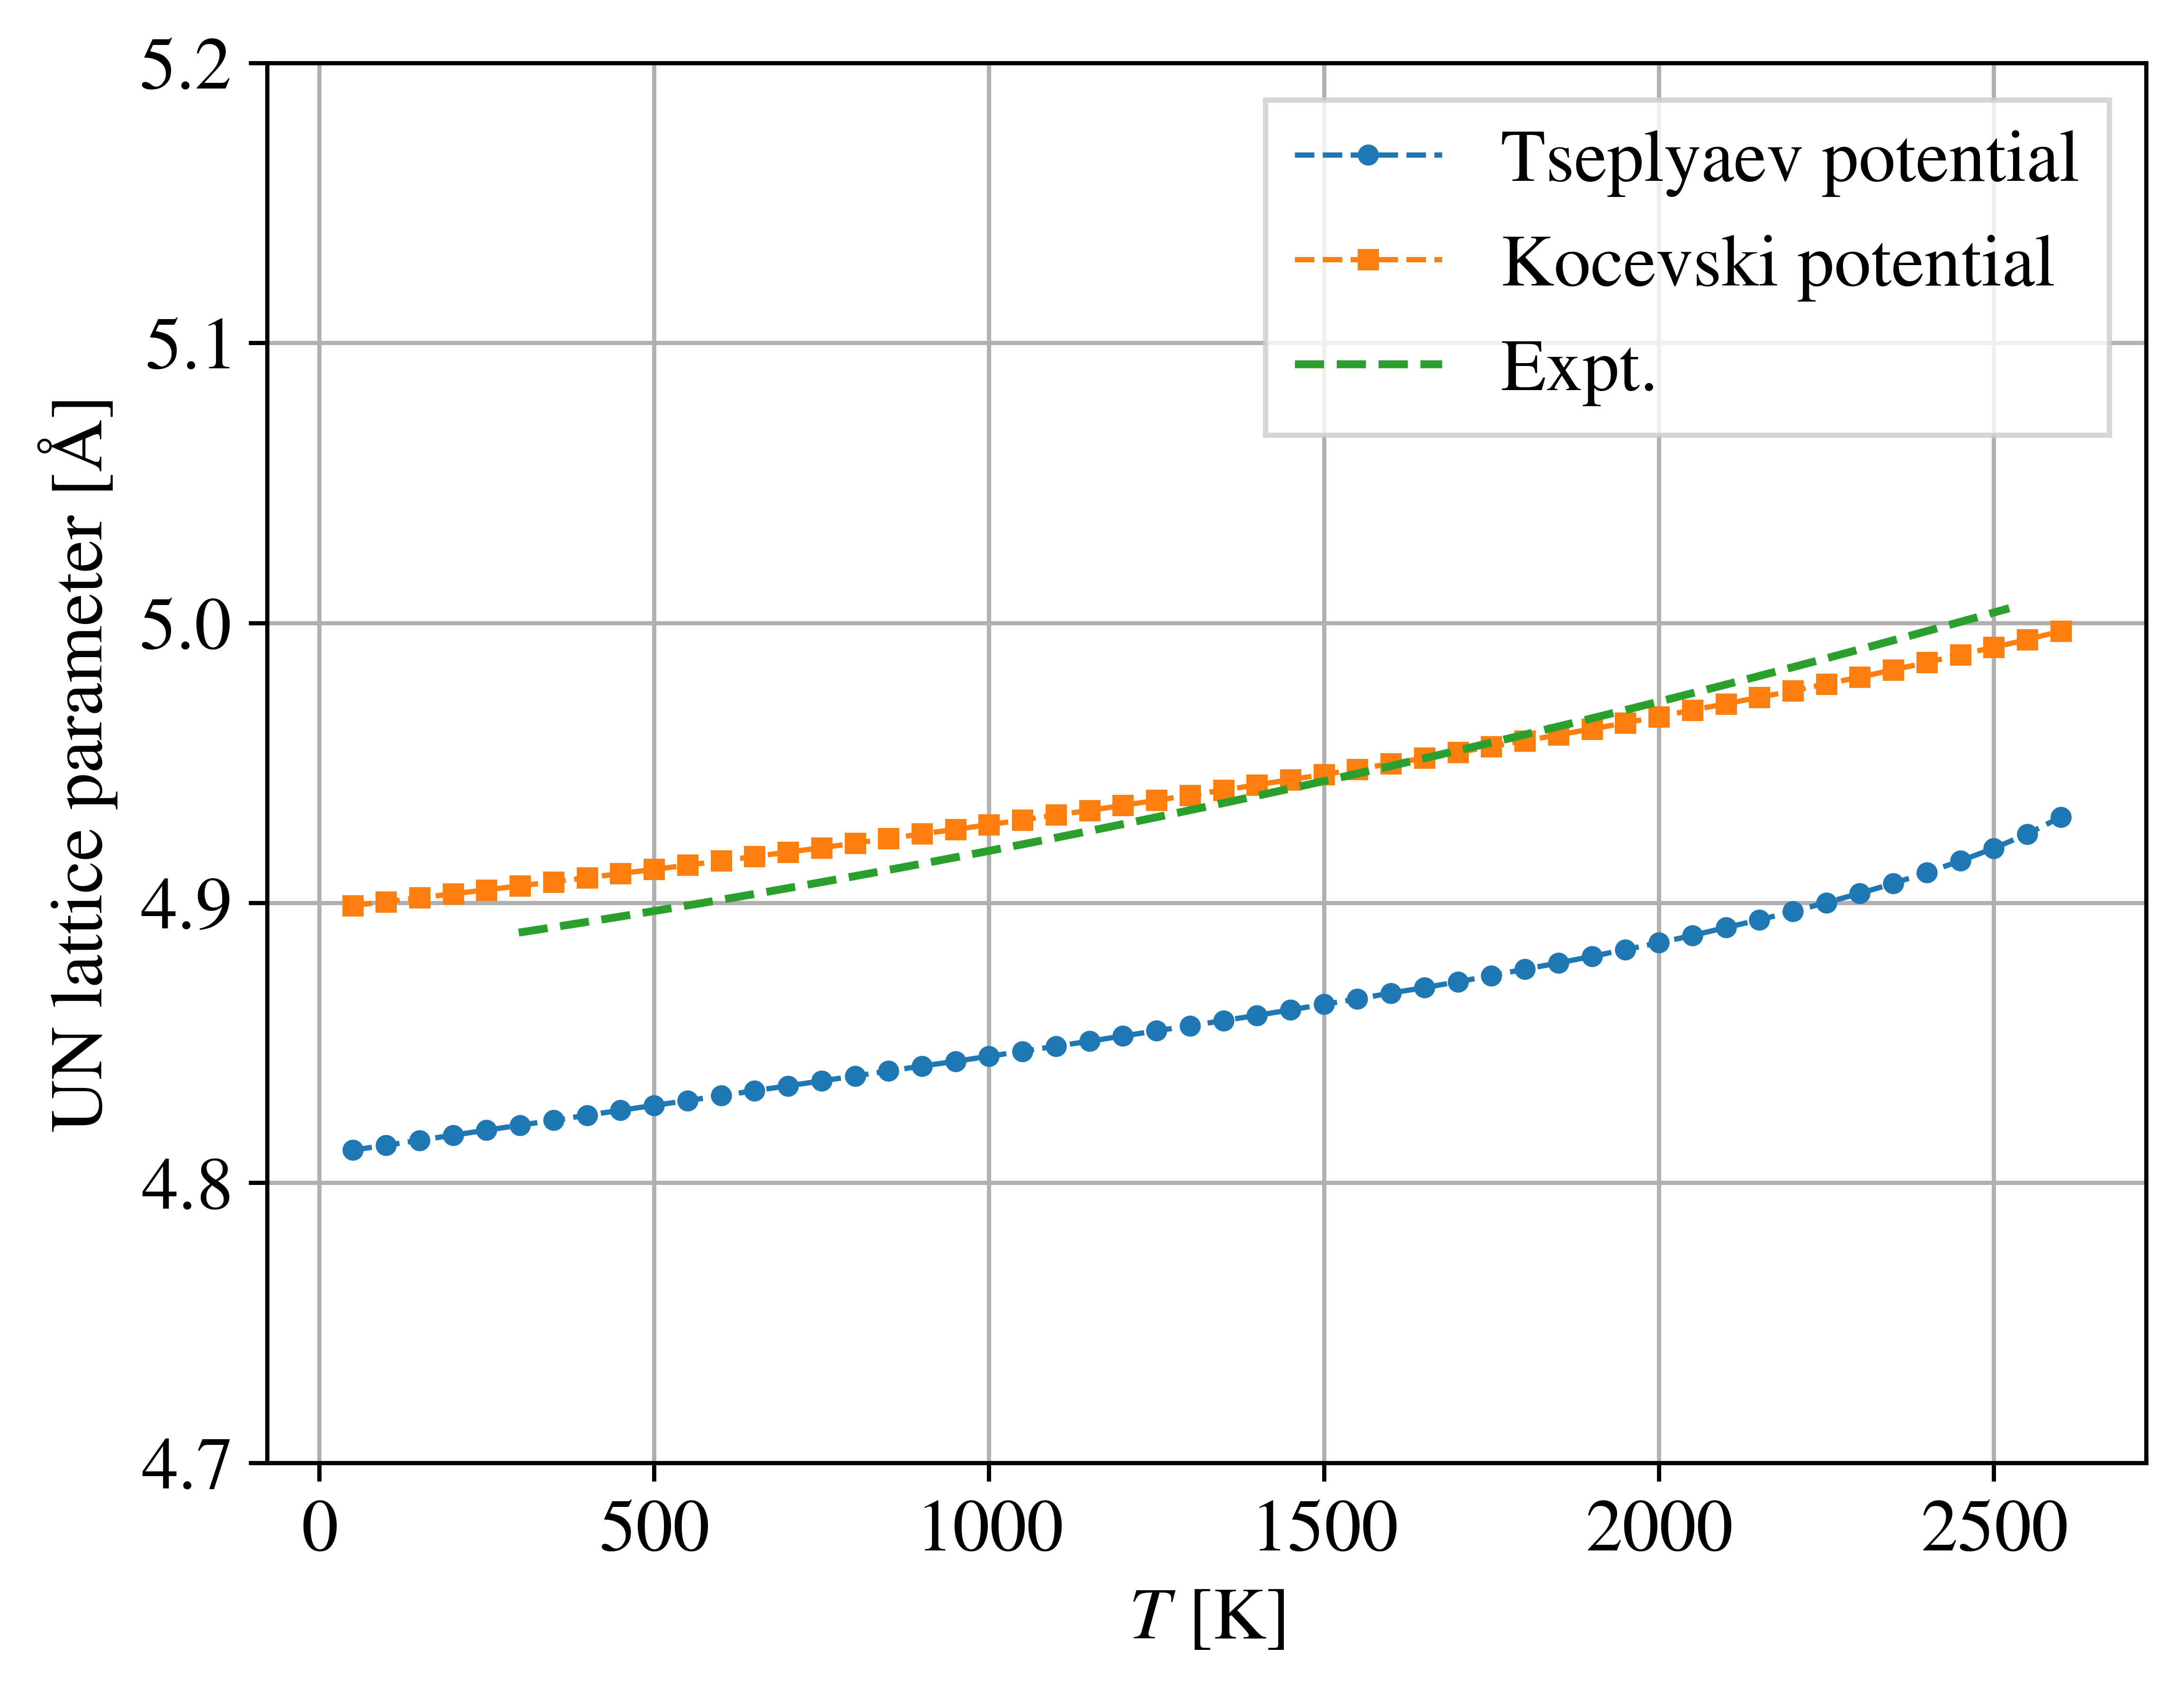
\includegraphics[width=\textwidth]{UNL.png}
    \caption{}
    \label{Fig:UNL}
\end{subfigure}
%\hfill
\begin{subfigure}{0.4\textwidth}
    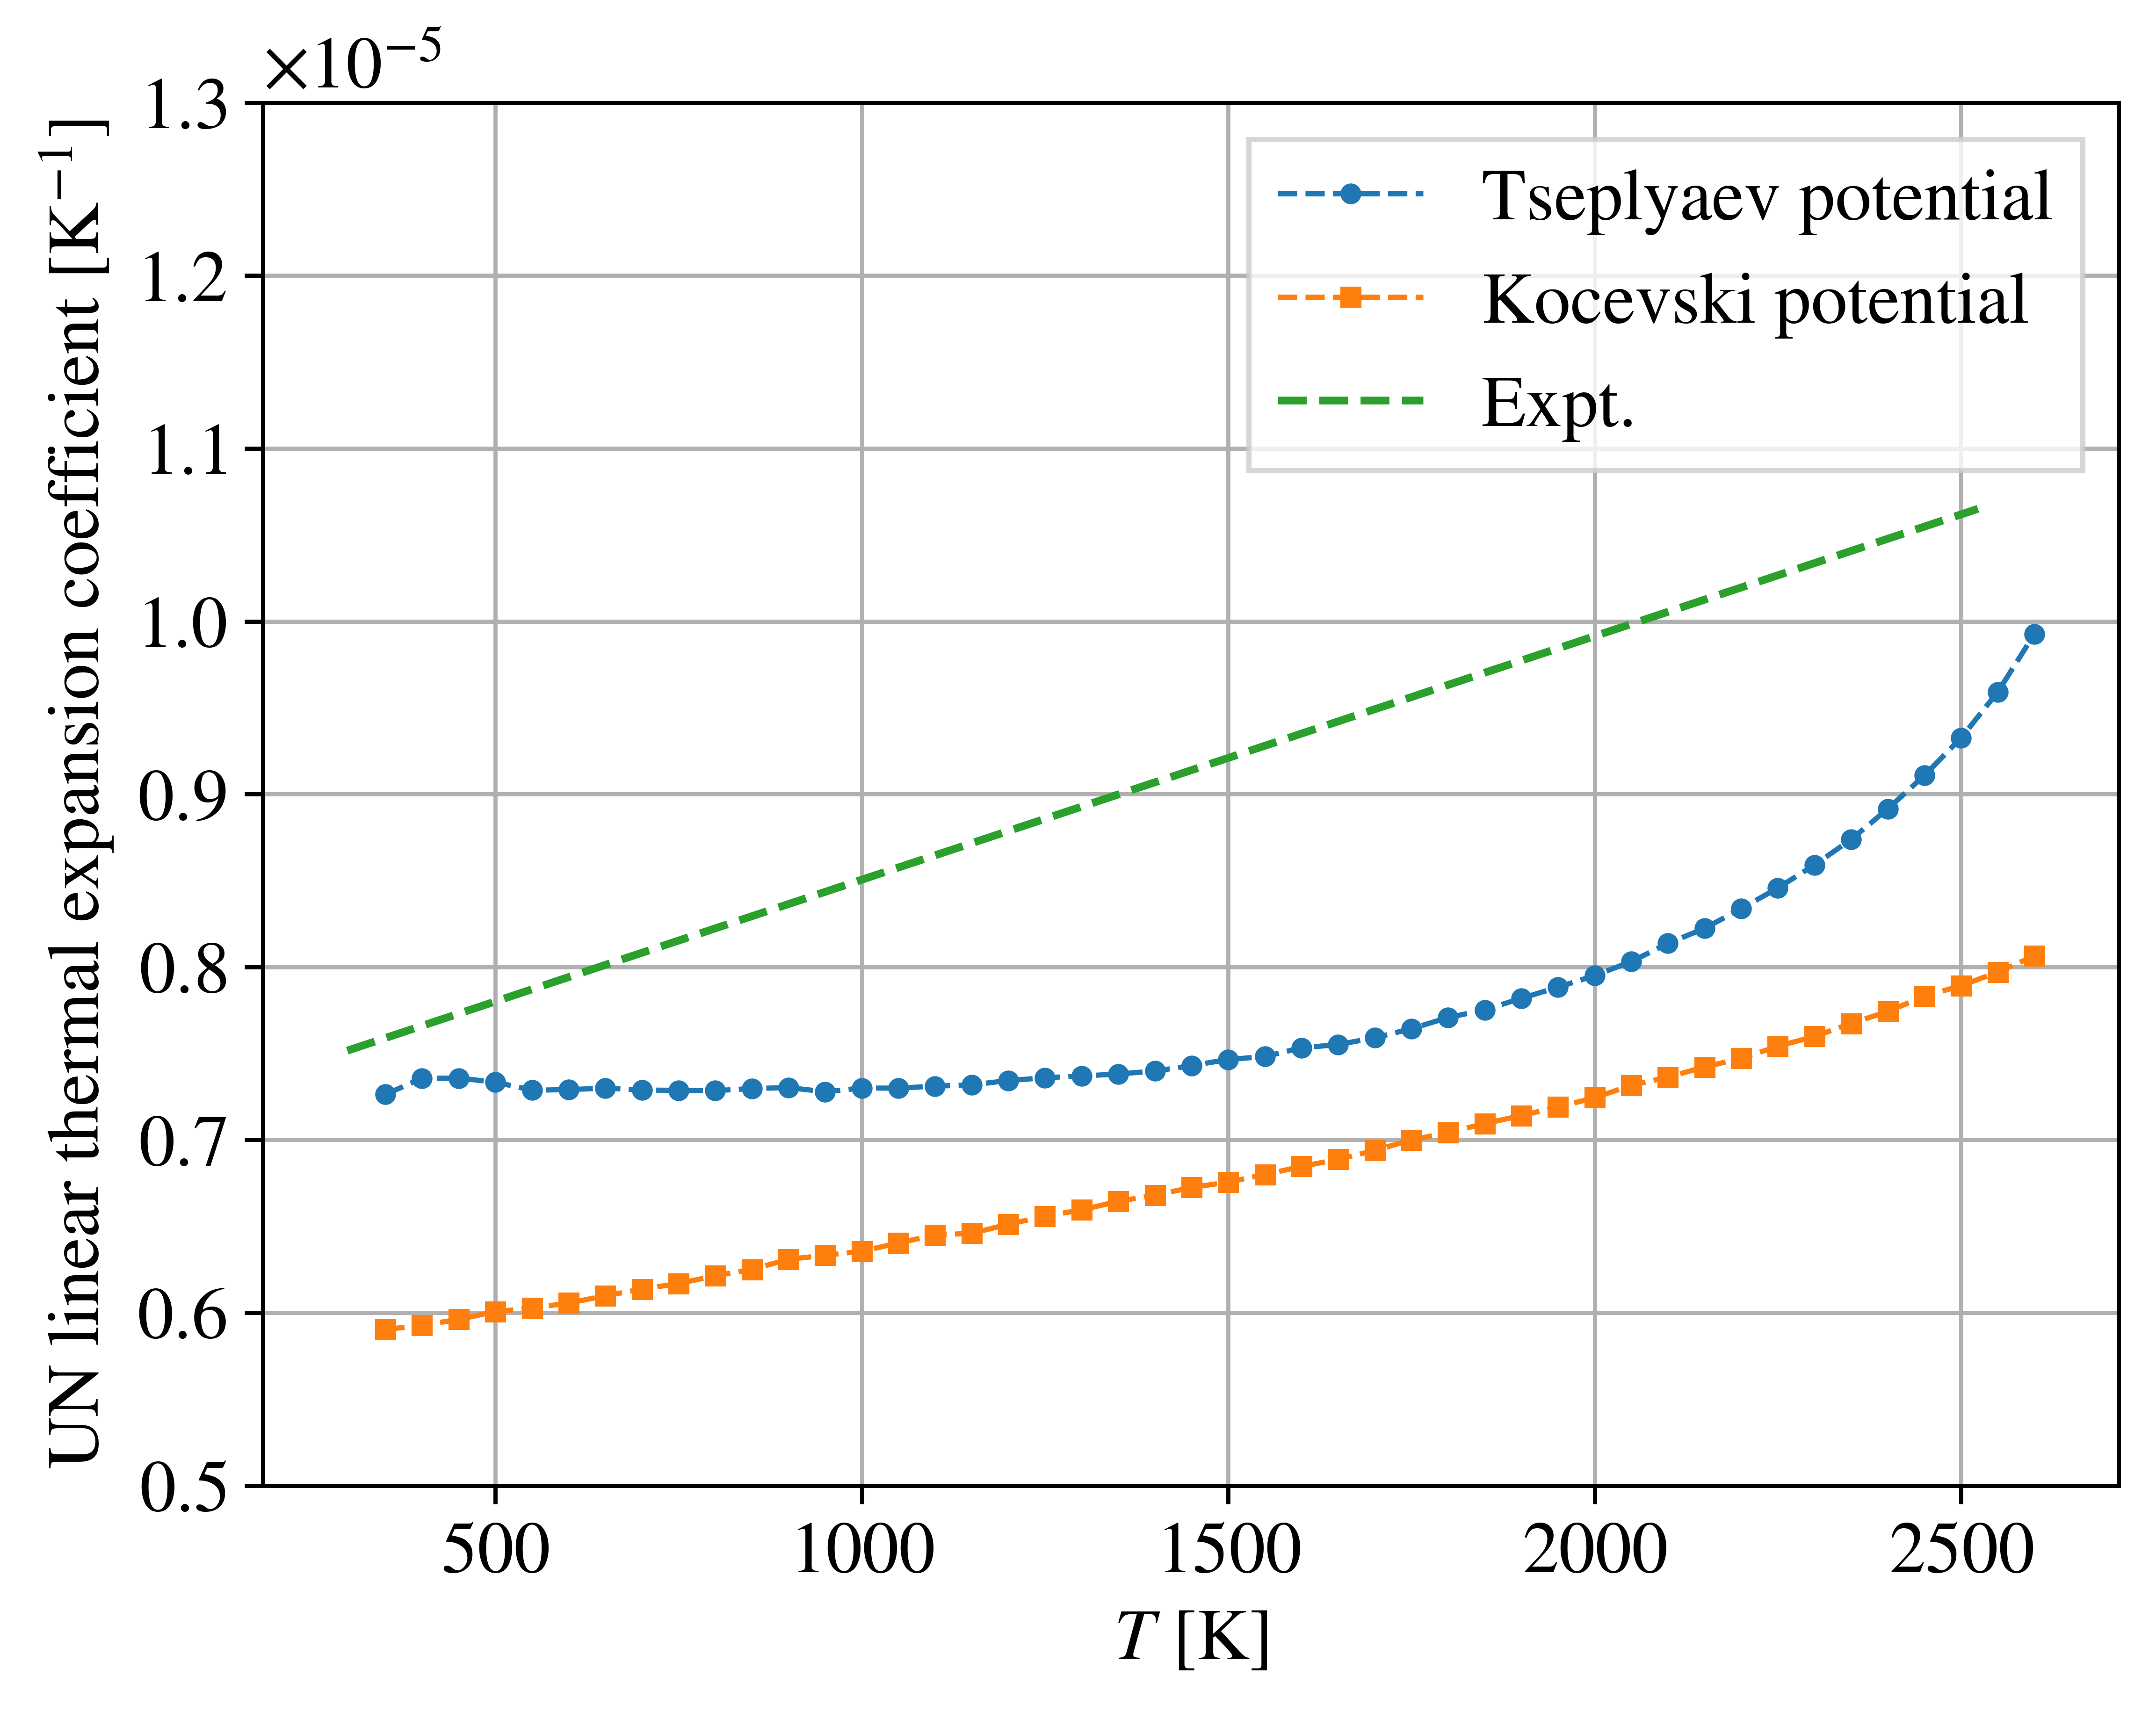
\includegraphics[width=\textwidth]{UNLTEC.png}
    \caption{}
    \label{Fig:UNLTEC}
\end{subfigure}
\caption{\textbf{(a)} UN lattice parameter calculated by both potentials and compared to the empirical correlation of Hayes \textit{et al.} (1990) \cite{Hayes1990I}. \textbf{(b)} UN linear thermal expansion coefficient calculated by both potentials and compared to the experimental data of Hayes \textit{et al.} (1990) \cite{Hayes1990I}.}
\label{Fig:UNL-LTEC}
\end{figure*}



\subsection{Melting point}

The melting temperature predicted by both potentials is shown in \cref{Fig:Tm}. According to Alavi and Thompson \cite{Alavi2006}, the thermodynamic melting point is determined as the value of the range over which the melting temperature appears to be independent of the void fraction. Based on this measure, the Tseplyaev potential predicts thermodynamic melting at about 2700 K, whereas the Kocevski potential predicts it at about 3100 K; a value that is close to the experimental value of 3035 K estimated from the Hayes \textit{et al.} correlation at a nitrogen vapor pressure of 1 atm \cite{Hayes1990IV}. It can be concluded that the Kocevski potential gives a better prediction of the phase stability range of UN because its predicted melting point is closer to the experimental data, whereas the Tseplyaev potential predicts a slightly premature melting of UN.

\begin{figure}[h!]
\centering
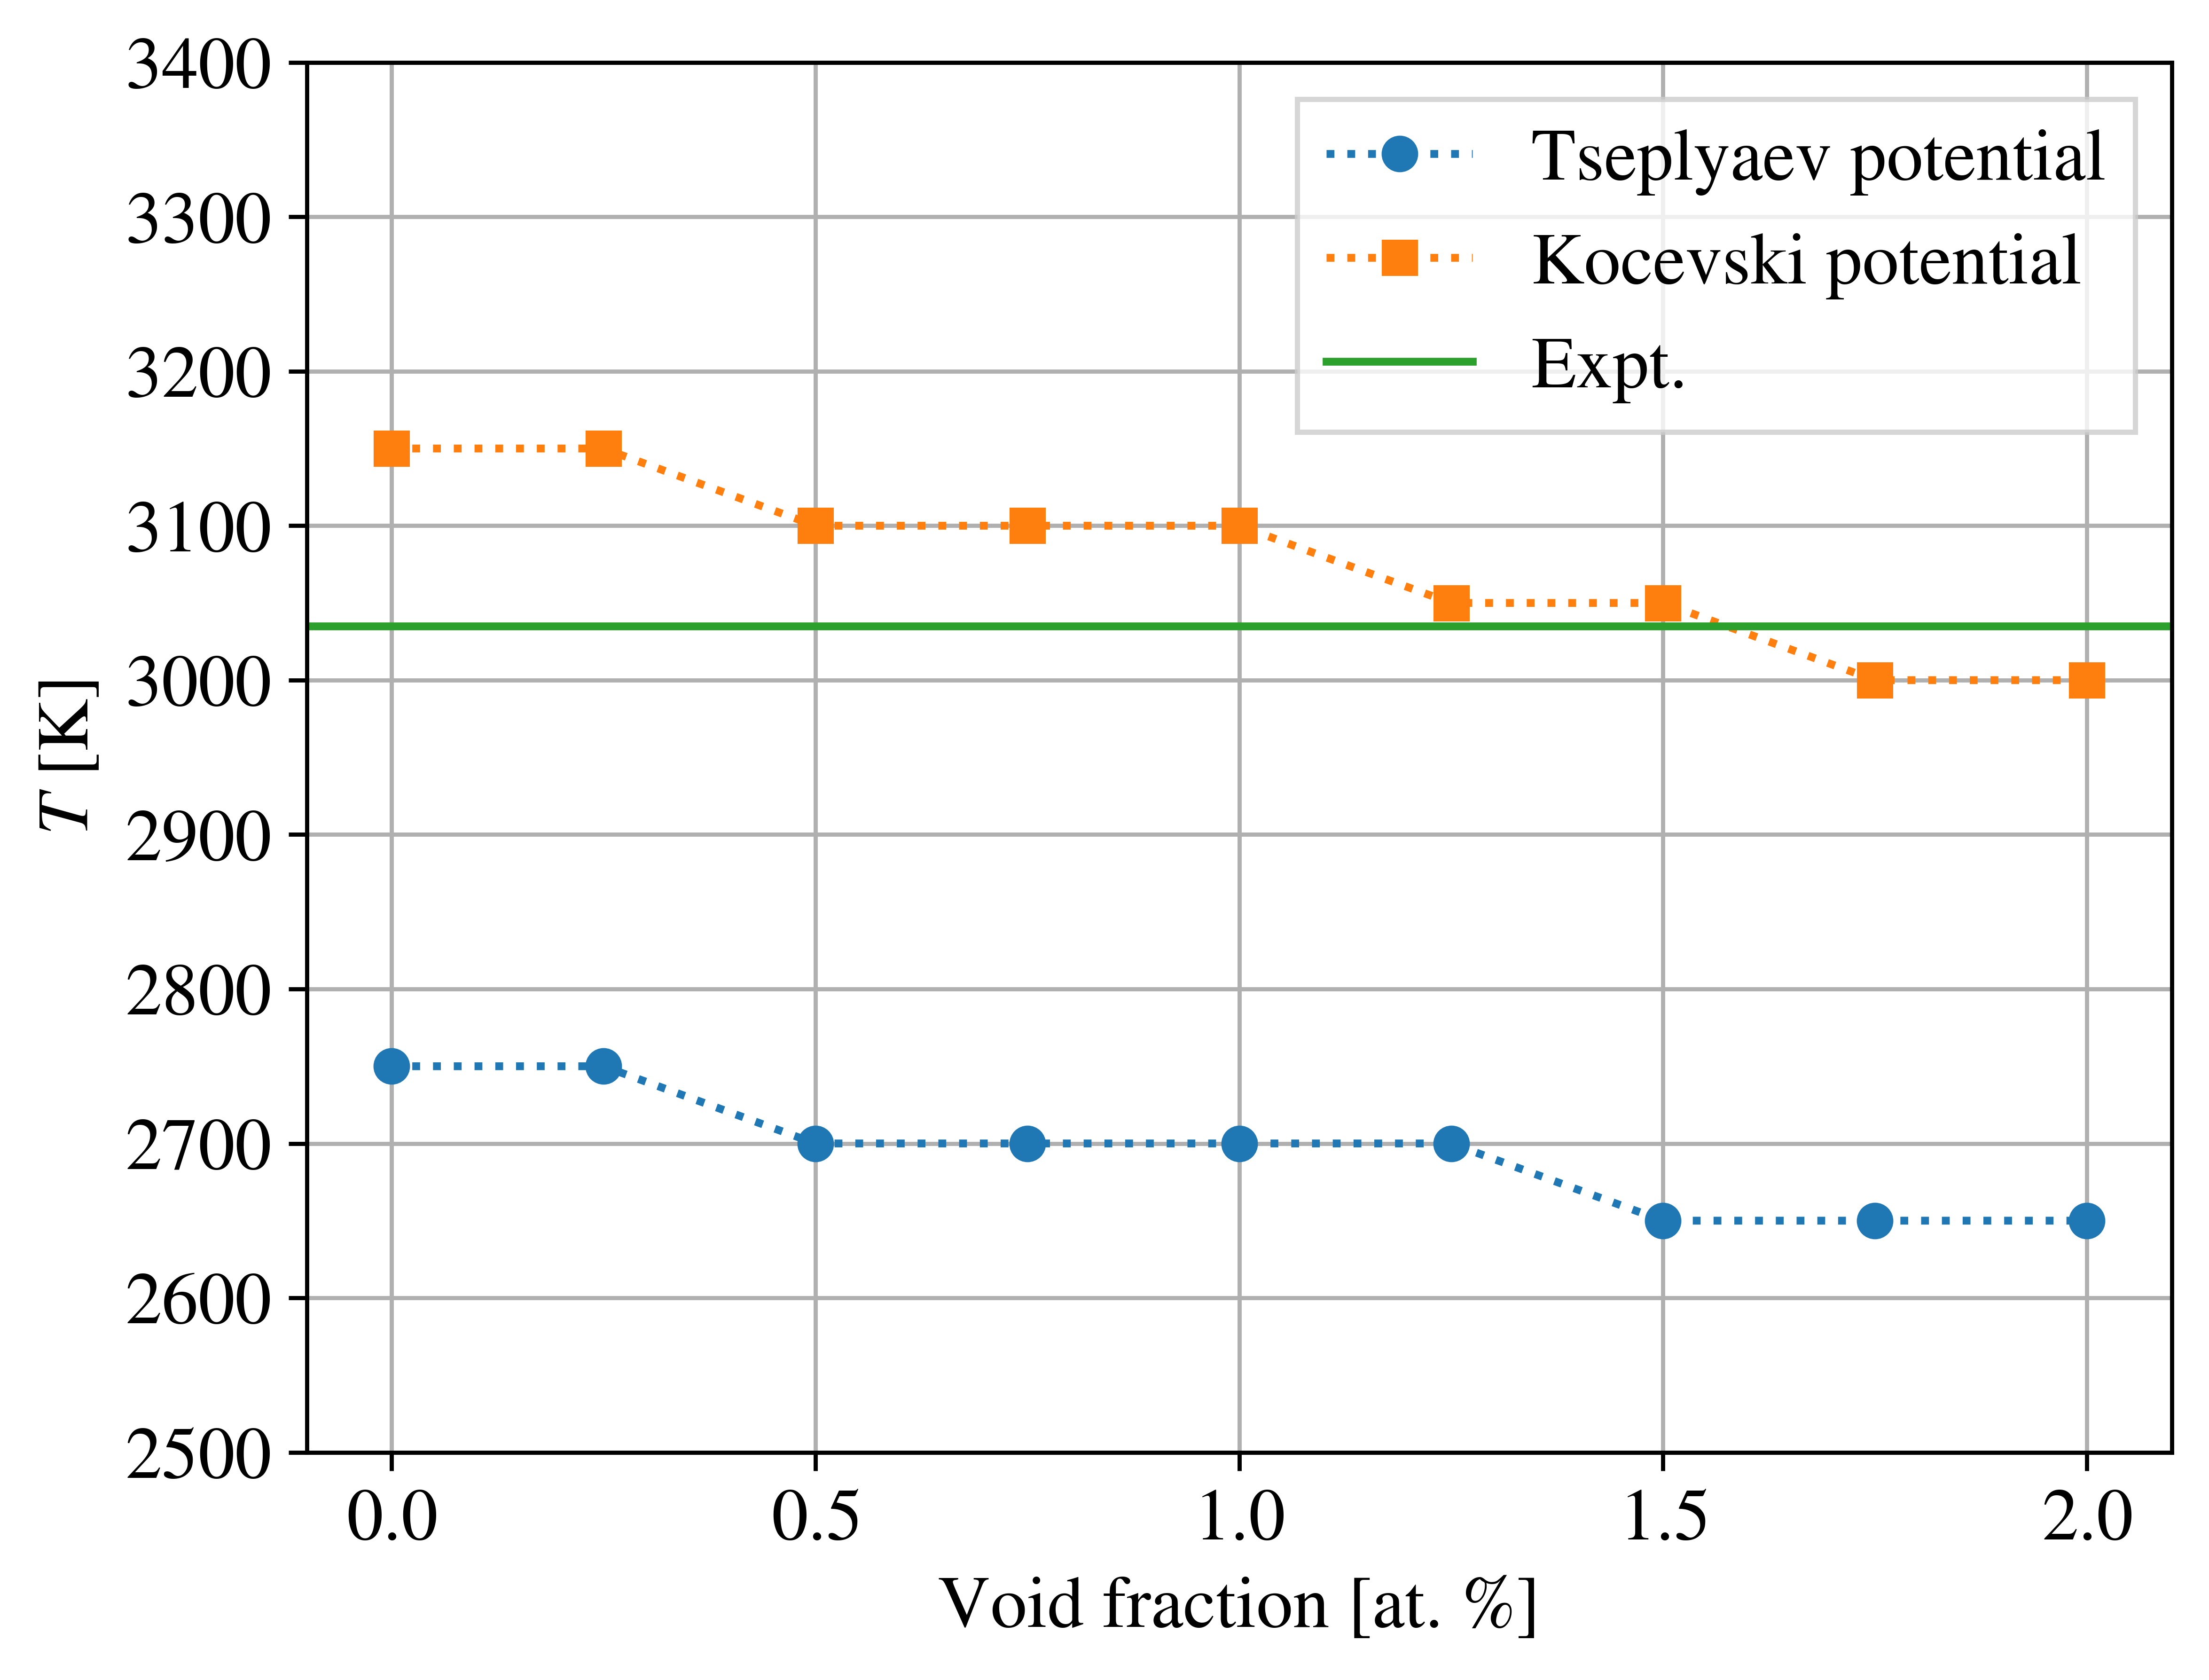
\includegraphics[width=0.5\textwidth]{Tm.png}
\caption{UN melting point as predicted by both potentials as a function of void fraction using the void-induced melting method. The experimental melting temperature (3035 K) is taken from the Hayes \textit{et al.} correlation at a nitrogen vapor pressure of 1 atm \cite{Hayes1990IV}.}
\label{Fig:Tm}
\end{figure}



\subsection{Elastic properties}
\label{Sec:Elastic}

The UN elastic constants calculated at 0 K using both potentials are shown in \cref{Tab:ElasticConst}. A much larger error is associated with the values of $C_{11}$ and $C_{44}$ calculated by the Tseplyaev potential compared to those calculated by the Kocevski potential, whereas the Tseplyaev potential estimation of $C_{12}$ is slightly better. It was found that UN elastic constants calculated at 0 K using the Tseplyaev potential show a discontinuity compared to finite-temperature values, which contradicts the third law of thermodynamics that requires a near-zero slope of the elastic constants versus $T$ curves as $T$ approaches 0 K \cite{Wachtman1961}. This discontinuity can be attributed to static energy minimization predicting metastable states of strained UN supercells. Thermal motion is likely to lead the strained supercells to a global minimum of the potential energy hypersurface. For this reason, we also compute the elastic constants at 1 K. The elastic constants, moduli, and Poisson's ratio at finite temperatures are shown in \cref{Fig:EC}. When calculated by the Kocevski potential, 1 K elastic constants show no significant difference from those calculated at 0 K, whereas 1 K elastic constants calculated by the Tseplyaev potential led to the disappearance of the discontinuity. All computed elastic constants were found to be independent of the amount of strain within the computational uncertainty.

\begin{table}[h!]
    \centering
    \footnotesize
    \caption{UN elastic constants (GPa) as calculated by both potentials. Experimental elastic constants are at 290 K.}
    \begin{tabular}{ccccc}
    \hline
                               & $C_{11}$ & $C_{12}$ & $C_{44}$ & $B$   \\
    \hline
    Tseplyaev potential (0 K)          & 586.6    & 110.5    & 54.7     & 269.2 \\
    Tseplyaev potential (1 K)          & 602.1    & 125.5    & 54.9     & 284.4 \\
    Kocevski potential (0 K) & 425.4    & 117.0    & 71.0     & 219.8 \\
    Expt. \cite{Salleh1986}    & 423.9    & 98.1     & 75.7     & 206.7 \\
    \hline
    \end{tabular}
    \label{Tab:ElasticConst}
\end{table}

\begin{figure}[h!]
\centering
\begin{subfigure}{0.49\textwidth}
    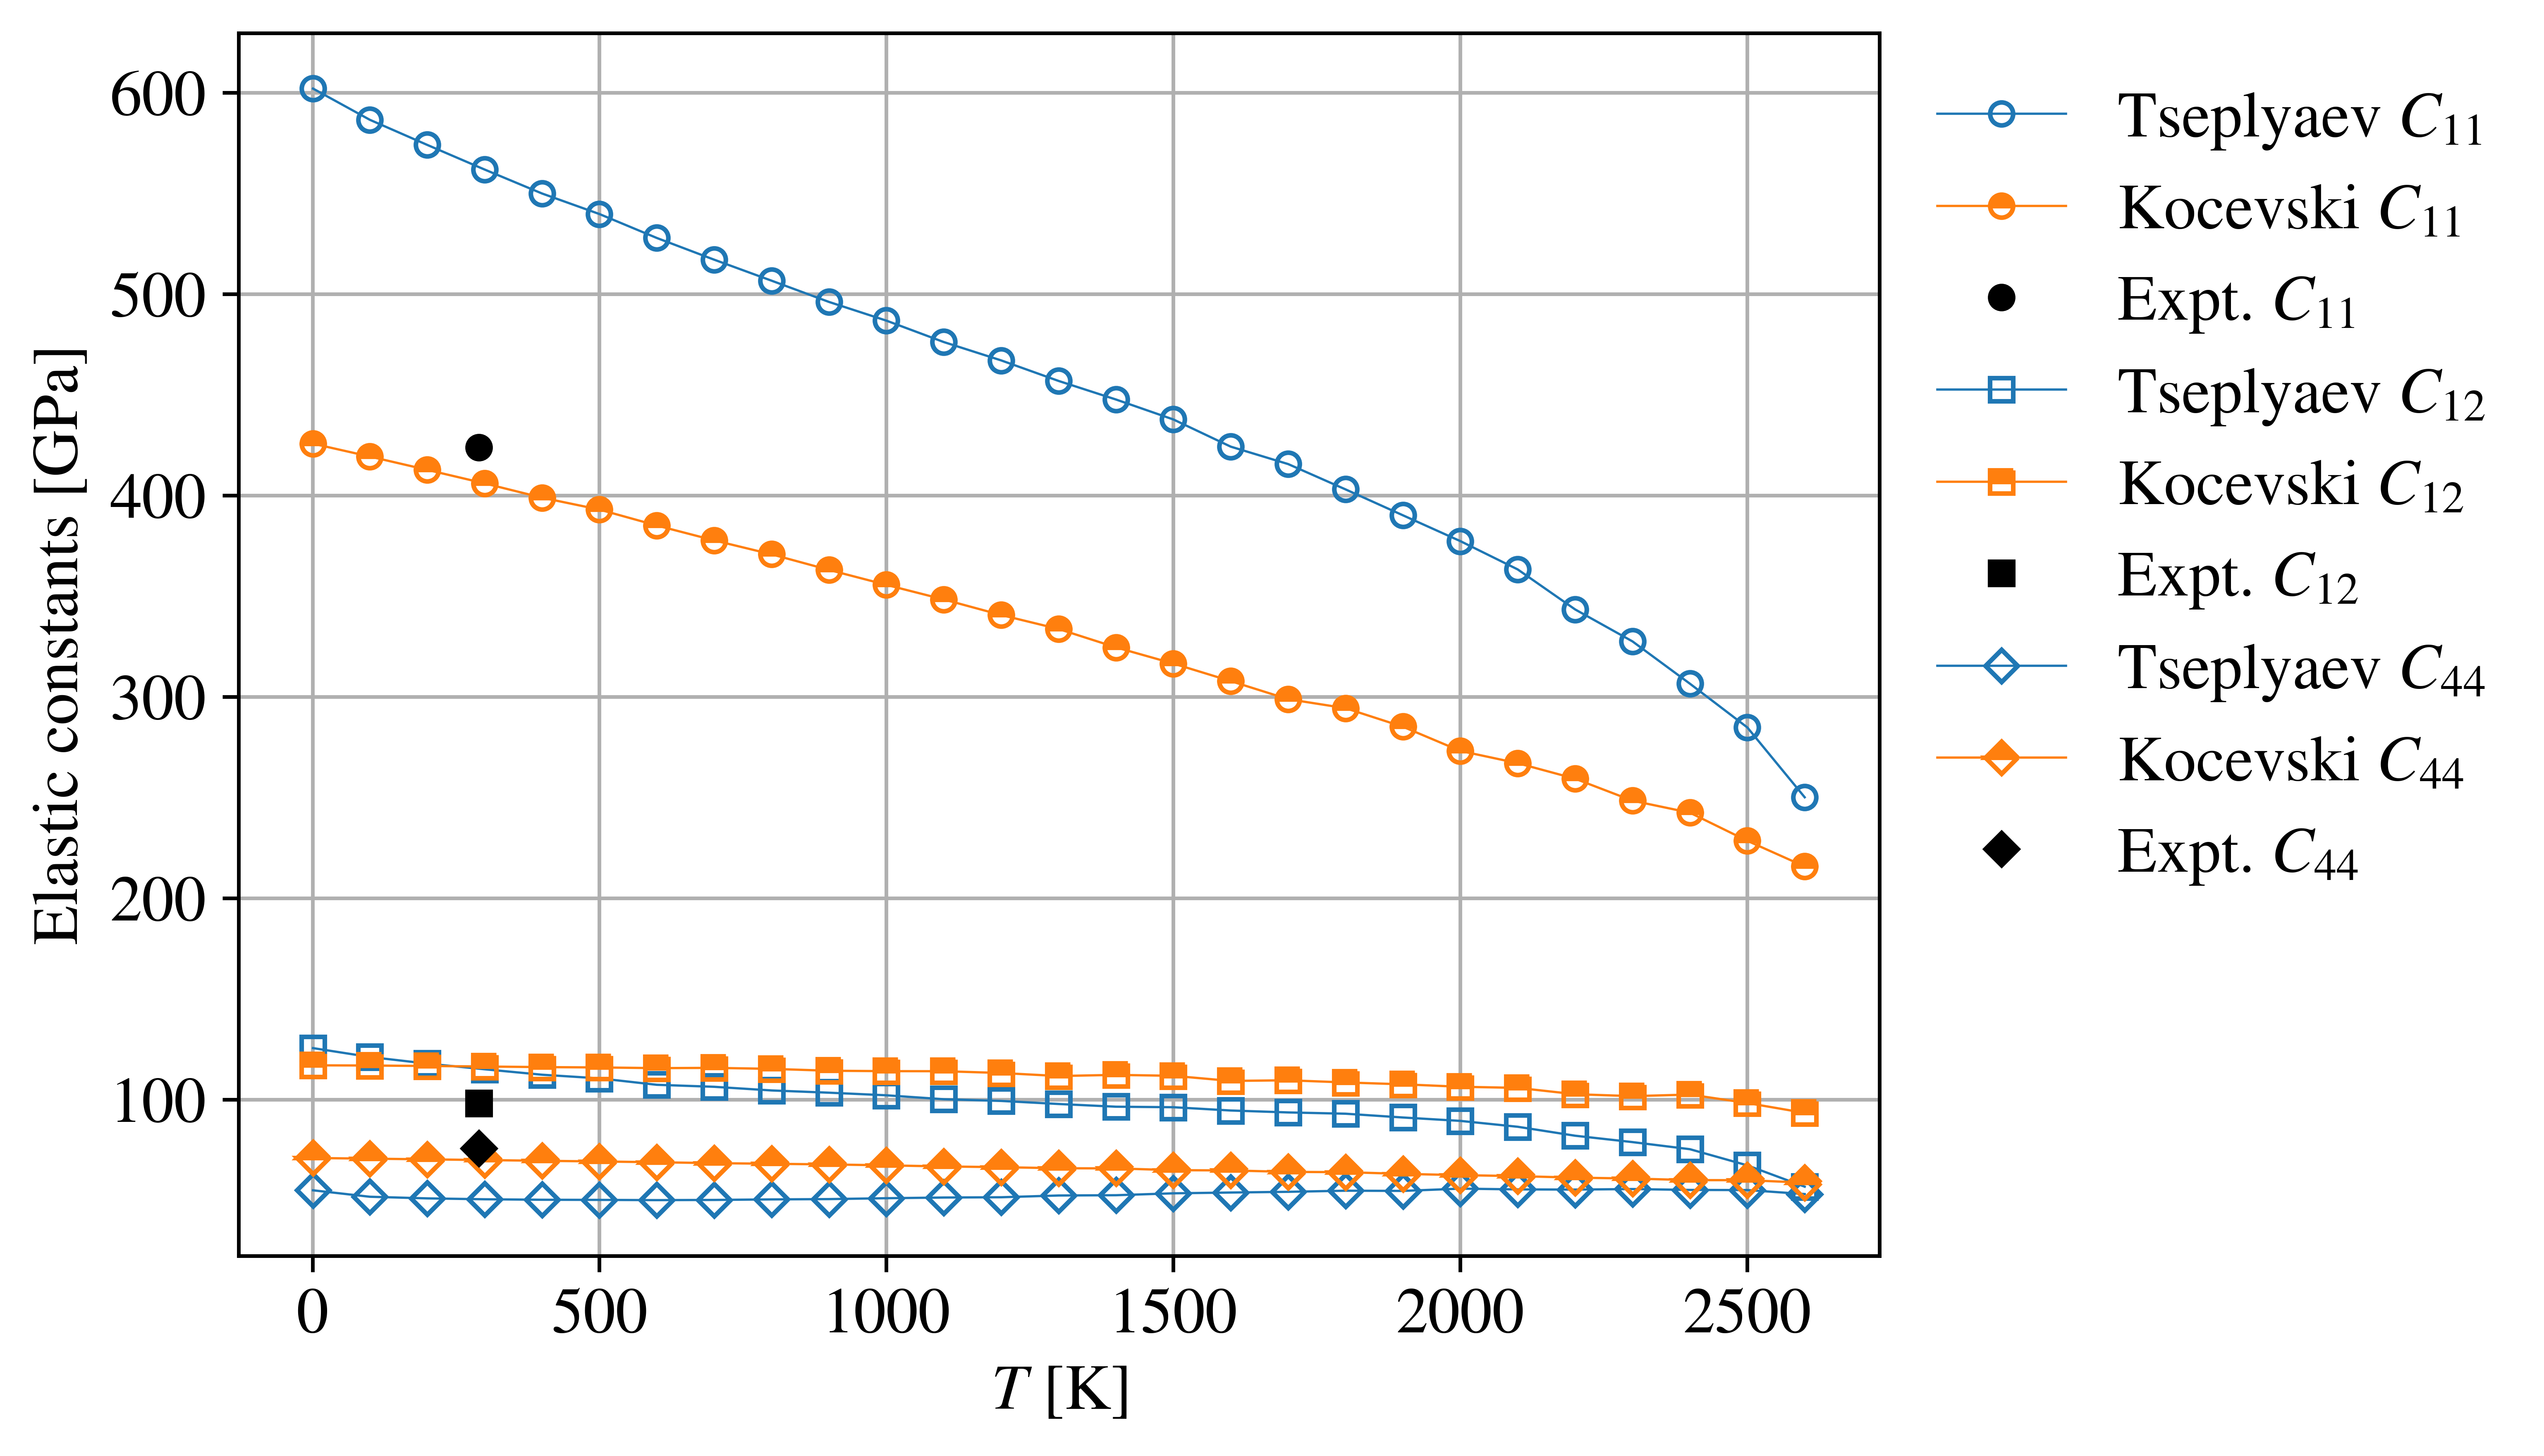
\includegraphics[width=\textwidth]{ElasticConstants.png}
    \caption{}
    \label{Fig:ElasConst}
\end{subfigure}
\hfill
\begin{subfigure}{0.49\textwidth}
    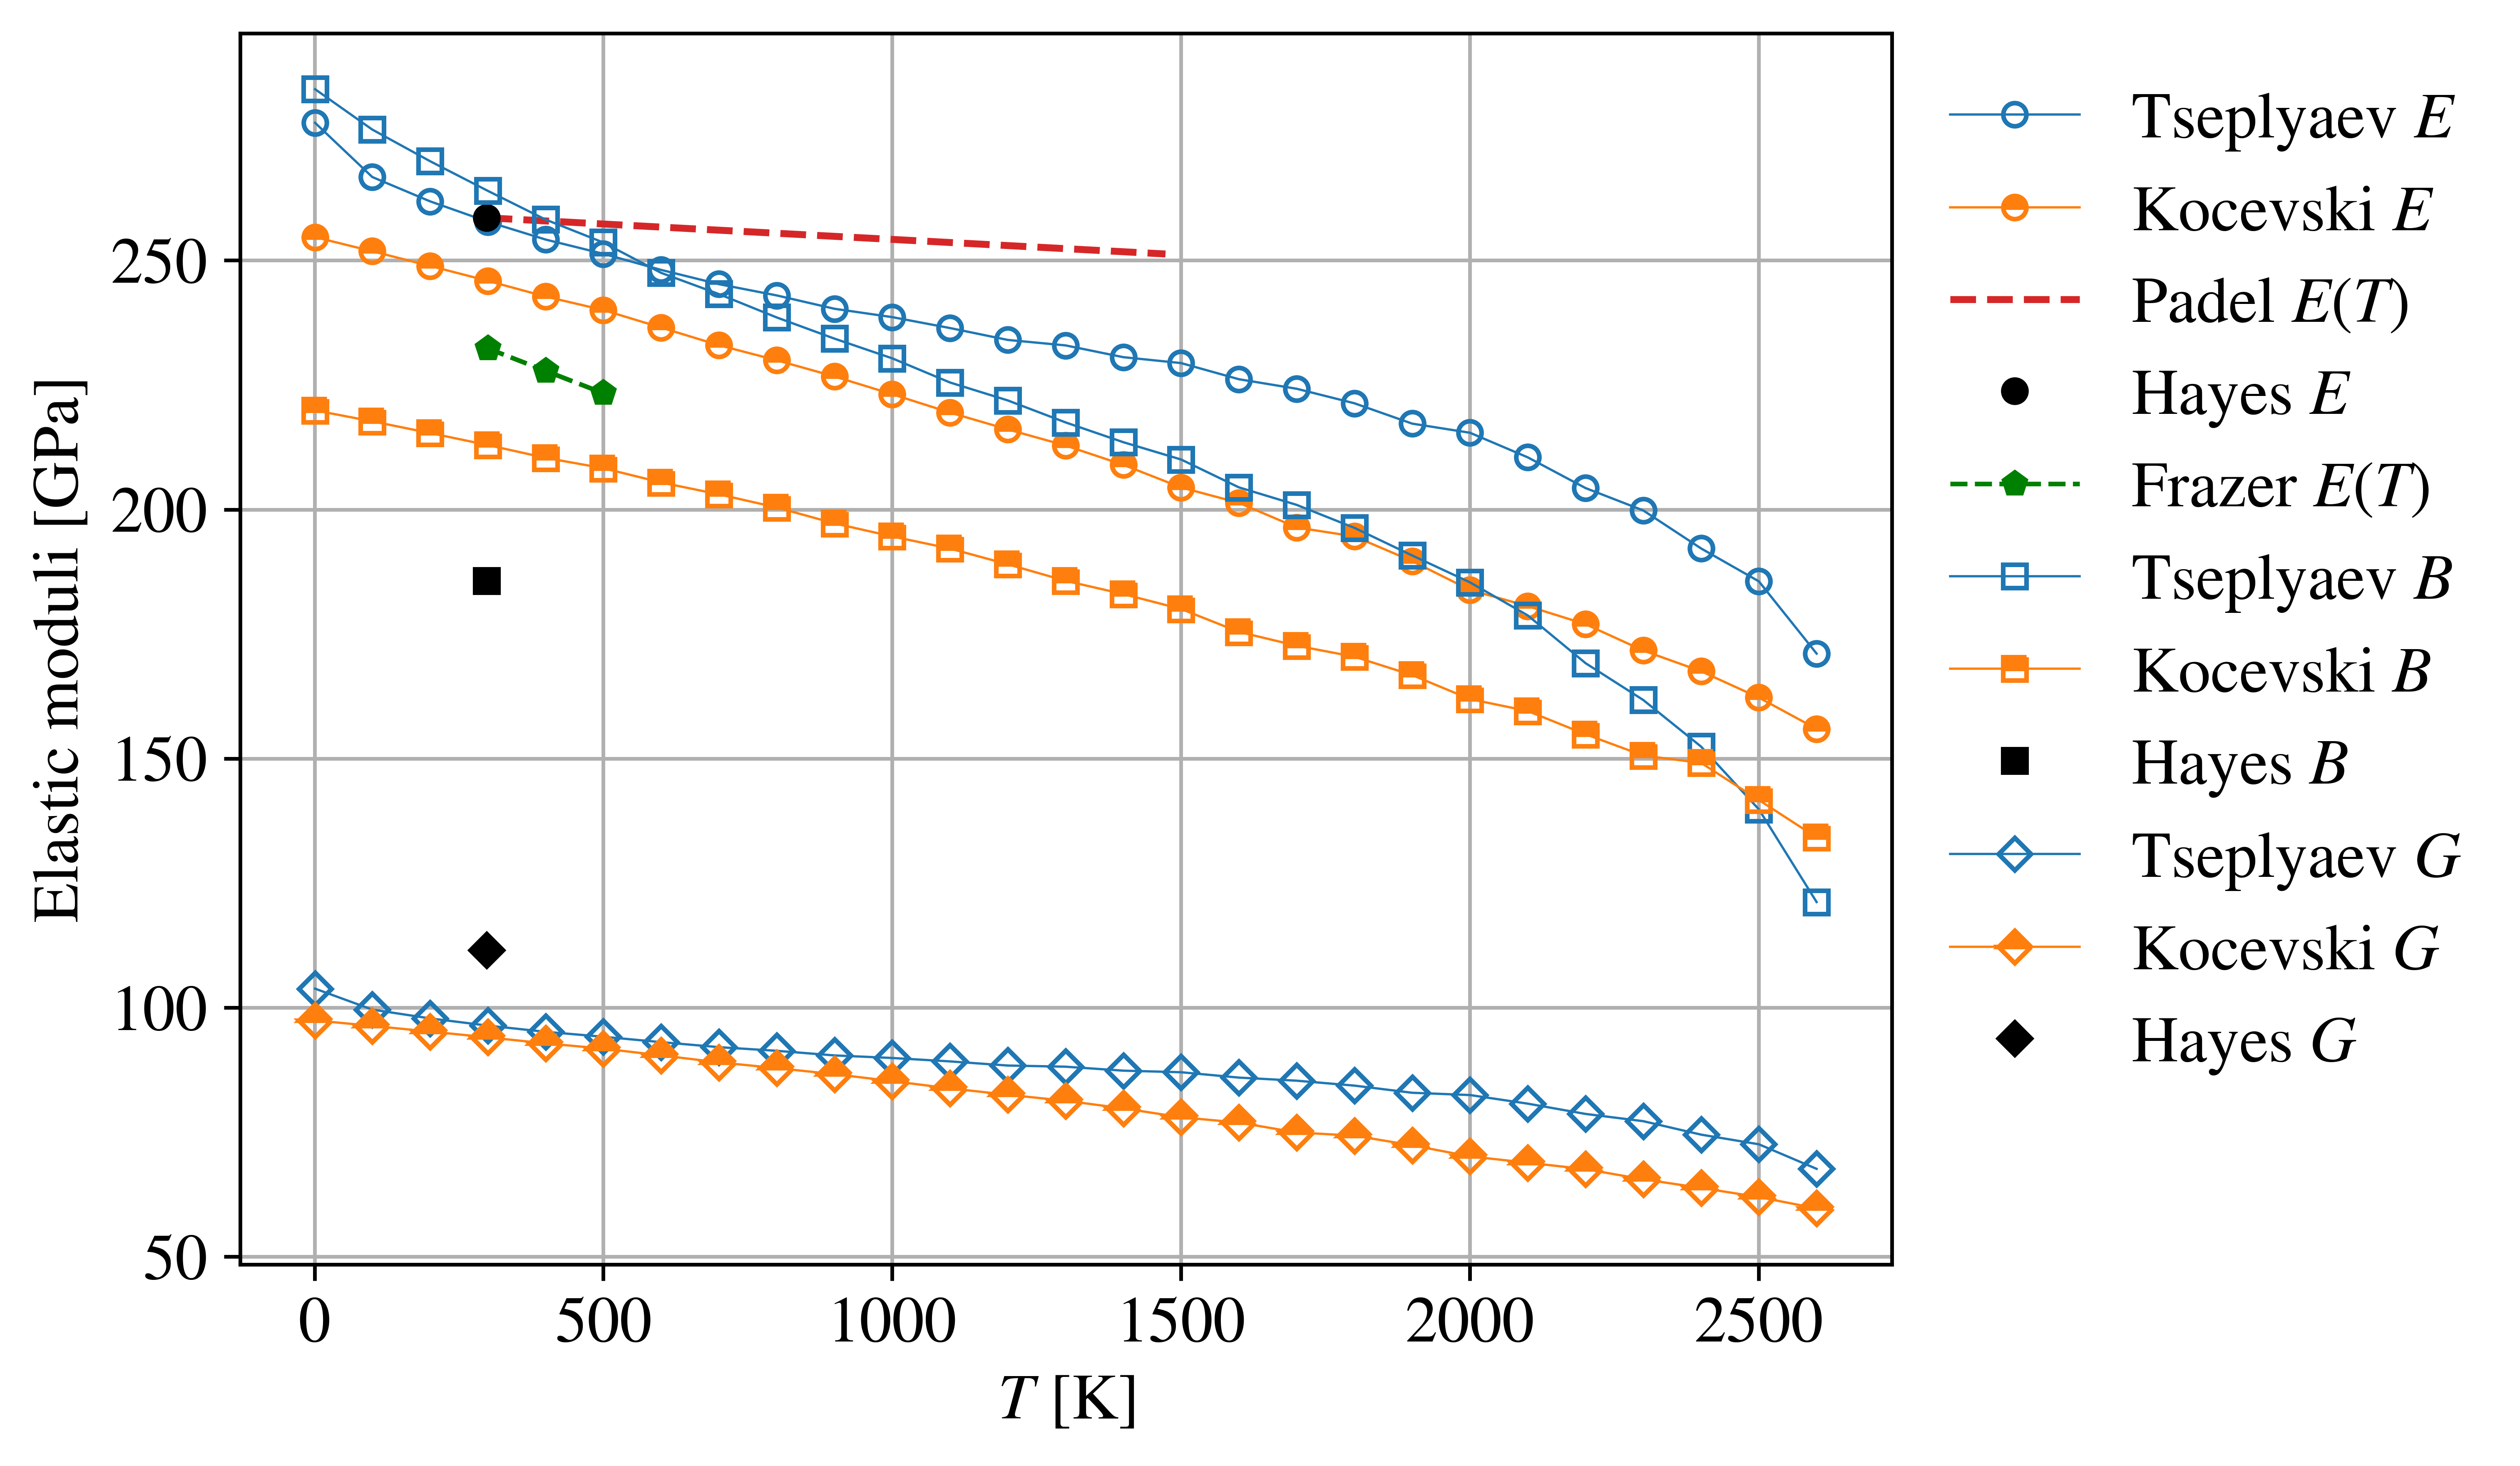
\includegraphics[width=\textwidth]{ElasticModuli.png}
    \caption{}
    \label{Fig:ElasMod}
\end{subfigure}
\hfill
\begin{subfigure}{0.45\textwidth}
    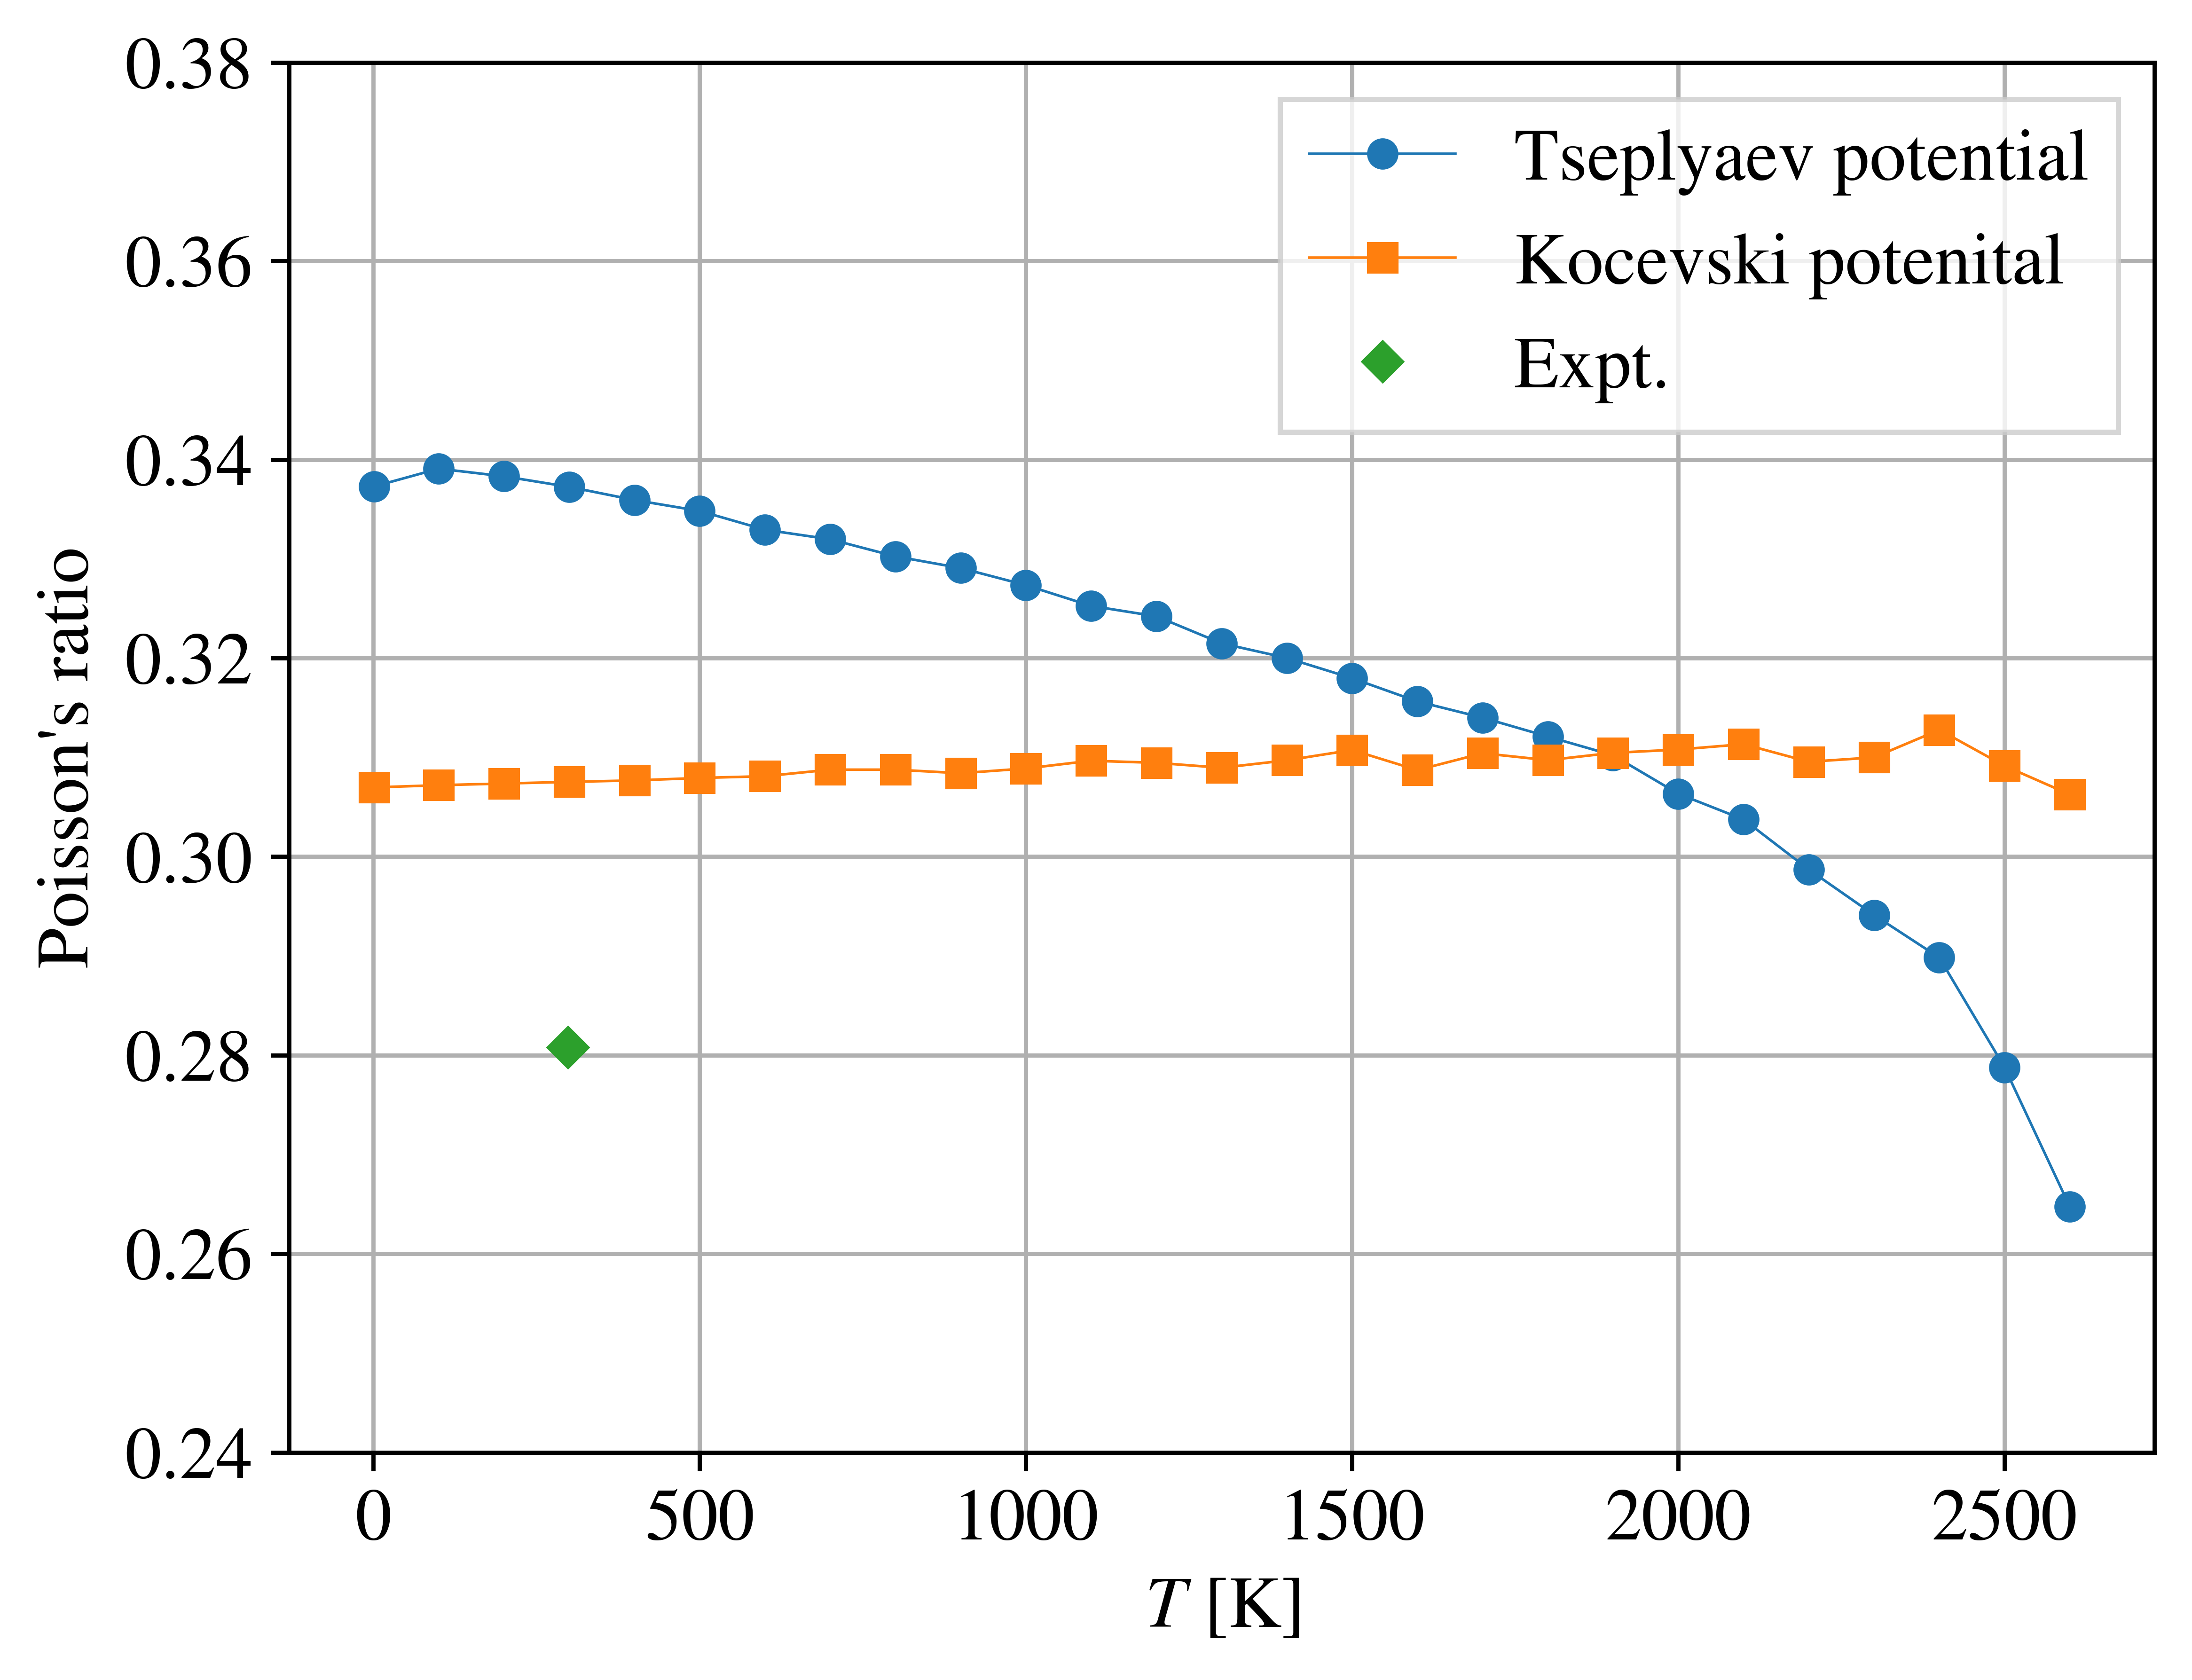
\includegraphics[width=\textwidth]{PoissonRatio.png}
    \caption{}
    \label{Fig:Poisson}
\end{subfigure}
\caption{Computations of the temperature variation of \textbf{(a)} UN elastic constants, $C_{11}$, $C_{12}$, and $C_{44}$, \textbf{(b)} UN Young's modulus, $E$, bulk modulus, $B$, and shear modulus, $G$, and \textbf{(c)} Poisson's ratio as calculated by both potentials. The experimental data points in \textbf{(a)} are from Salleh \textit{et al.} (1986) \cite{Salleh1986}. The experimental data points in \textbf{(b)} and \textbf{(c)} are from Hayes \textit{et al.} (1990) \cite{Hayes1990II}. The experimental variation of Young's modulus with temperature in \textbf{(b)} is due to Padel and de Novion \cite{Padel1969}, which Hayes \textit{et al.} assumed to be valid also for UN's bulk and shear moduli, and due to the more recent study by Frazer \textit{et al.} \cite{Frazer2021}.}
\label{Fig:EC}
\end{figure}

In \cref{Fig:ElasConst}, $C_{12}$ and $C_{44}$ computed by the Tseplyaev potential show a good agreement with experimental values at RT, whereas it overestimates RT $C_{11}$ by more than 35\%. On the other hand, all elastic constants calculated by the Kocevski potential agree well with the experimental values at RT. Regarding the elastic moduli (\cref{Fig:ElasMod}), the Tseplyaev potential reproduces the experimental Young's modulus by Hayes \textit{et al.} \cite{Hayes1990II} at RT, while the RT value calculated by the Kocevski potential can be regarded as an average estimate of the value of Hayes \textit{et al.} \cite{Hayes1990II} and Frazer \textit{et al.} \cite{Frazer2021}. The Tseplyaev potential overestimates the UN bulk modulus by more than 40\%, whereas the Kocevski potential shows a better prediction and only overestimates it by about 15\%. Both potentials slightly underestimate the shear modulus, $G$. The Kocevski potential shows a good prediction of the UN Poisson's ratio compared to the experimental value at RT (\cref{Fig:Poisson}) and predicts a slight increase with increasing temperature, which is the expected trend. However, the Tseplyaev potential predicts a decrease of the Poisson's ratio with increasing temperature, related to the significant softening of the bulk modulus.

The only experimental measurements of the temperature variation of the UN elastic properties are the studies by Padel and de Novion \cite{Padel1969} and by Frazer \textit{et al.} \cite{Frazer2021} on the temperature dependence of UN Young's modulus. Padel and de Novion \cite{Padel1969} report a temperature dependence of Young's modulus of the form:
\begin{equation}
E(T)= E_0 \left( 1-2.375 \times 10^{-5} T \right)
\label{Eq:Padel}
\end{equation}
in the temperature range of 298-1473 K, with no experimental data to support it, whereas Frazer \textit{et al.} predict a dependence of the form:
\begin{equation}
E(T) = 245.78 - 0.0449 T
\label{Eq:Frazer}
\end{equation}
in the temperature range of 300-500 K.

\cref{Eq:Padel} predicts a softening rate that is much slower than that predicted by either potential as is obvious in \cref{Fig:ElasMod}, whereas, despite its limited range, the softening rate implied by Frazer \textit{et al.}'s data \cite{Frazer2021} seems to agree better with that predicted by both potentials. Hayes \textit{et al.} \cite{Hayes1990II} assumed the temperature dependence of \cref{Eq:Padel} applies for all elastic properties except for Poisson's ratio, which they assumed to be independent of temperature. This latter assumption agrees with Poisson's ratio calculated by the Kocevski potential which can be approximated as temperature-independent. Kocevski \textit{et al.} \cite{Kocevski2022II} also calculated the temperature variation of the UN elastic properties using their potential. Our results generally agree with theirs for all elastic properties except for Poisson's ratio which they estimated to be $\sim$0.22 at RT compared to the experimental value of $\sim$0.28 and our value of 0.31. The reason for this discrepancy is that they calculated Poisson's ratio from the formula: $\nu = C_{12}/\left( C_{11}+C_{12} \right)$, which assumes the elastic constants are of an isotropic material which is not the case for UN, as $C_{11}-C_{12} \neq 2C_{44}$ \cite{Salleh1986, Zener1947}.

The computed Debye temperatures using different methods are given in \cref{Tab:Debye} and compared to values reported in the literature. Values calculated in this work fall within the range 355-368 K and agree with the values calculated by Scarbrough \textit{et al.} \cite{Scarbrough1968} and Whaley \textit{et al.} \cite{Whaley1969}. A large scatter is evident in the experimental Debye temperature values which range from 181-364 K. Scarbrough \textit{et al.} \cite{Scarbrough1968} suspected that the values reported by Counsell \textit{et al.} \cite{Counsell1964} and Westrum and Barber \cite{Westrum1966} (276 K and 289 K, respectively) are likely affected by the presence of magnetic specific heat. Salleh \textit{et al.} \cite{Salleh1986} report a value of $\theta_D$ = 282 K without any reference to the method they used to derive it. It's interesting to note that when Salleh \textit{et al.}'s RT elastic constants are substituted into the Anderson and Siethoff-Ahlborn methods, they give values of $\theta_D$ = 365 K and $\theta_D$ = 373 K, respectively.

\begin{table}[h!]
    \centering
    \footnotesize    
    \caption{UN Debye temperature values estimated in this work and reported in the literature.}
    \begin{tabular}{llc}
    \hline
    Method                                  & Reference & $\theta_{D}$ \\
    \hline
    Tseplyaev potential + Anderson method             & This work & 365 K \\
    Tseplyaev potential + Siethoff-Ahlborn method     & This work & 356 K \\ 
    Kocevski potential + Anderson method              & This work & 355 K \\
    Kocevski potential + Siethoff-Ahlborn method      & This work & 356 K \\
    \hline
    Sound-velocity measurements in polycrystalline UN             & Whaley \textit{et al.} \cite{Whaley1969}     & 361-364 K \\
    Specific heat measurements in the temperature range 1.3-4.6 K & Scarbrough \textit{et al.} \cite{Scarbrough1968} & 324 K \\
    Specific heat measurements in the temperature range 5-350 K   & Westrum and Barber \cite{Westrum1966}   & 289 K \\
    Specific heat measurements in the temperature range 11-320 K  & Counsell \textit{et al.} \cite{Counsell1964}     & 276 K \\
    Not reported                                          & Salleh \textit{et al.} \cite{Salleh1986}   & 282 K \\
    Derived from the UN phonon spectrum measured at 4.2 K & Baranov \textit{et al.} \cite{Baranov2013} & 181 K \\
    DFT calculation                                       & Mei \textit{et al.} \cite{Mei2013}         & 244 K \\
    \hline
    \end{tabular}
    \label{Tab:Debye}
\end{table}

Baranov \textit{et al.} \cite{Baranov2013} made a mistake in their estimation of the Debye temperature. They computed the Debye frequency using $\omega_D = v_0 k_D$, where $v_0$ is the average phonon group velocity estimated from \cref{Eq:v_m}  with $v_0$ = 2990 m/s (given that $v_l$ = 4740 m/s and $v_t$ = 2691 m/s) and $k_D = \left( 6 \pi^2 / \Omega \right)^{1/3}$, where $\Omega$, the volume of the primitive UN unit cell, is equal to $a^3/4$, $a$ being the lattice parameter \cite{Sellan2010}. Instead of using the volume of the \textit{primitive} UN unit cell, they used the volume of the conventional unit cell, which led to an underestimation of the Debye temperature $\theta_D = \hbar \omega_D / k_B$. Instead of $\theta_D$ = 181 K, their appropriate value should have been $\theta_D$ = 289 K. Interestingly, when using the formula $v_0 = \left( v_l + 2 v_t \right)/3$ to average the velocities of the acoustic branches \cite{Sellan2010}, $v_0$ = 3373 m/s and Baranov \textit{et al.}'s $\theta_D$ = 326 K, which is close to our calculated values. Based on this analysis, it can be concluded that the variation of the experimental Debye temperature between the two ranges 276-289 K and 324-365 K can partly be attributed to the differences in the averaging formulas used to estimate the average acoustic phonon group velocity. Another contribution is the antiferromagnetic nature of UN which leads the $\theta_D$ estimated from specific heat data to be smaller than that estimated from elastic constants as pointed out by Whaley \textit{et al.} \cite{Whaley1969}. Based on this analysis, we can conclude that the average UN $\theta_D$ is around 362 K as estimated from both experimental and computed elastic constants.



\subsection{Specific heat capacity}

UN $C_P$ and its components are shown in \cref{Fig:CVCP}. $C_{\mathrm{exp}}$ (\cref{Fig:CD}) is calculated from functions fitted to the UN LTEC (\cref{Eq:LTEC1,Eq:LTEC2}) and bulk modulus (\cref{Eq:B1,Eq:B2}), and $C_\mathrm{anharm}$ (\cref{Fig:Canharm}) is calculated from functions fitted to the values of $C_P$ (\cref{CPADP,CPEAM}) and $C_V$ (\cref{CVADP,CVEAM}) calculated by both potentials. It can be seen in \cref{Fig:UNCP} that the Tseplyaev potential compares well with the UN $C_P$ experimental correlation from Hayes \textit{et al.} \cite{Hayes1990IV}. However, care must be taken when comparing to the high-temperature values of this correlation as discussed by Galvin \textit{et al.} \cite{Galvin2023}. Both potentials agree in the computed $C_P$ and $C_V$ up to about 1200 K and 700 K, respectively, whereas at higher temperatures, the Kocevski potential significantly underestimates both $C_P$ and $C_V$. The Tseplyaev potential predicts that the anharmonic contribution is nearly zero at low and intermediate temperatures, and only becomes significant at $T >$ 1800 K, whereas the Kocevski potential predicts a minor contribution across the entire temperature spectrum. As can be seen in \cref{Fig:CVCP}, the discrepancy between the $C_P$ computed by both potentials ($\sim$30 J/mol-K at 2500 K) can almost completely be attributed to a difference in the computed $C_V$ ($\sim$10 J/mol-K at 2500 K) and a difference in the estimated $C_\mathrm{anharm}$ ($\sim$20 J/mol-K at 2500 K), whereas the difference in the thermal expansion contribution is quite small ($\sim$1 J/mol-K at 2500 K). It is interesting to note that the structural inaccuracies of the Tseplyaev potential in determining both the bulk modulus and the LTEC nearly balance and cancel out giving a $C_\mathrm{exp}$ value that is very close to that predicted by the Kocevski potential at low temperatures. That is, the Tseplyaev-potential predictions of UN properties are energetically accurate despite the observed structural and elastic inaccuracies.

% The slightly-below-zero part of $C_\mathrm{anharm}$ calculated by the ADP stems from the ADP $C_P$ being fitted to a $T^5$ functional form (\cref{CPADP}) whereas the ADP $C_V$ being fitted to a $T^{2.5}$ functional form (\cref{CVADP}). These values fall within the uncertainty of the calculation, i.e., are effectively zero, and have no physical significance.

$C_V$ and $C_\mathrm{anharm}$ are completely determined by the phonon properties of the material, and, thus, to understand why the Kocevski potential underestimates the UN $C_P$, a deeper investigation of the UN phonon properties as predicted by both potentials is necessary and will be shown in \cref{sub:phonon}.

\begin{figure}[h!]
\centering
\begin{subfigure}{0.45\textwidth}
    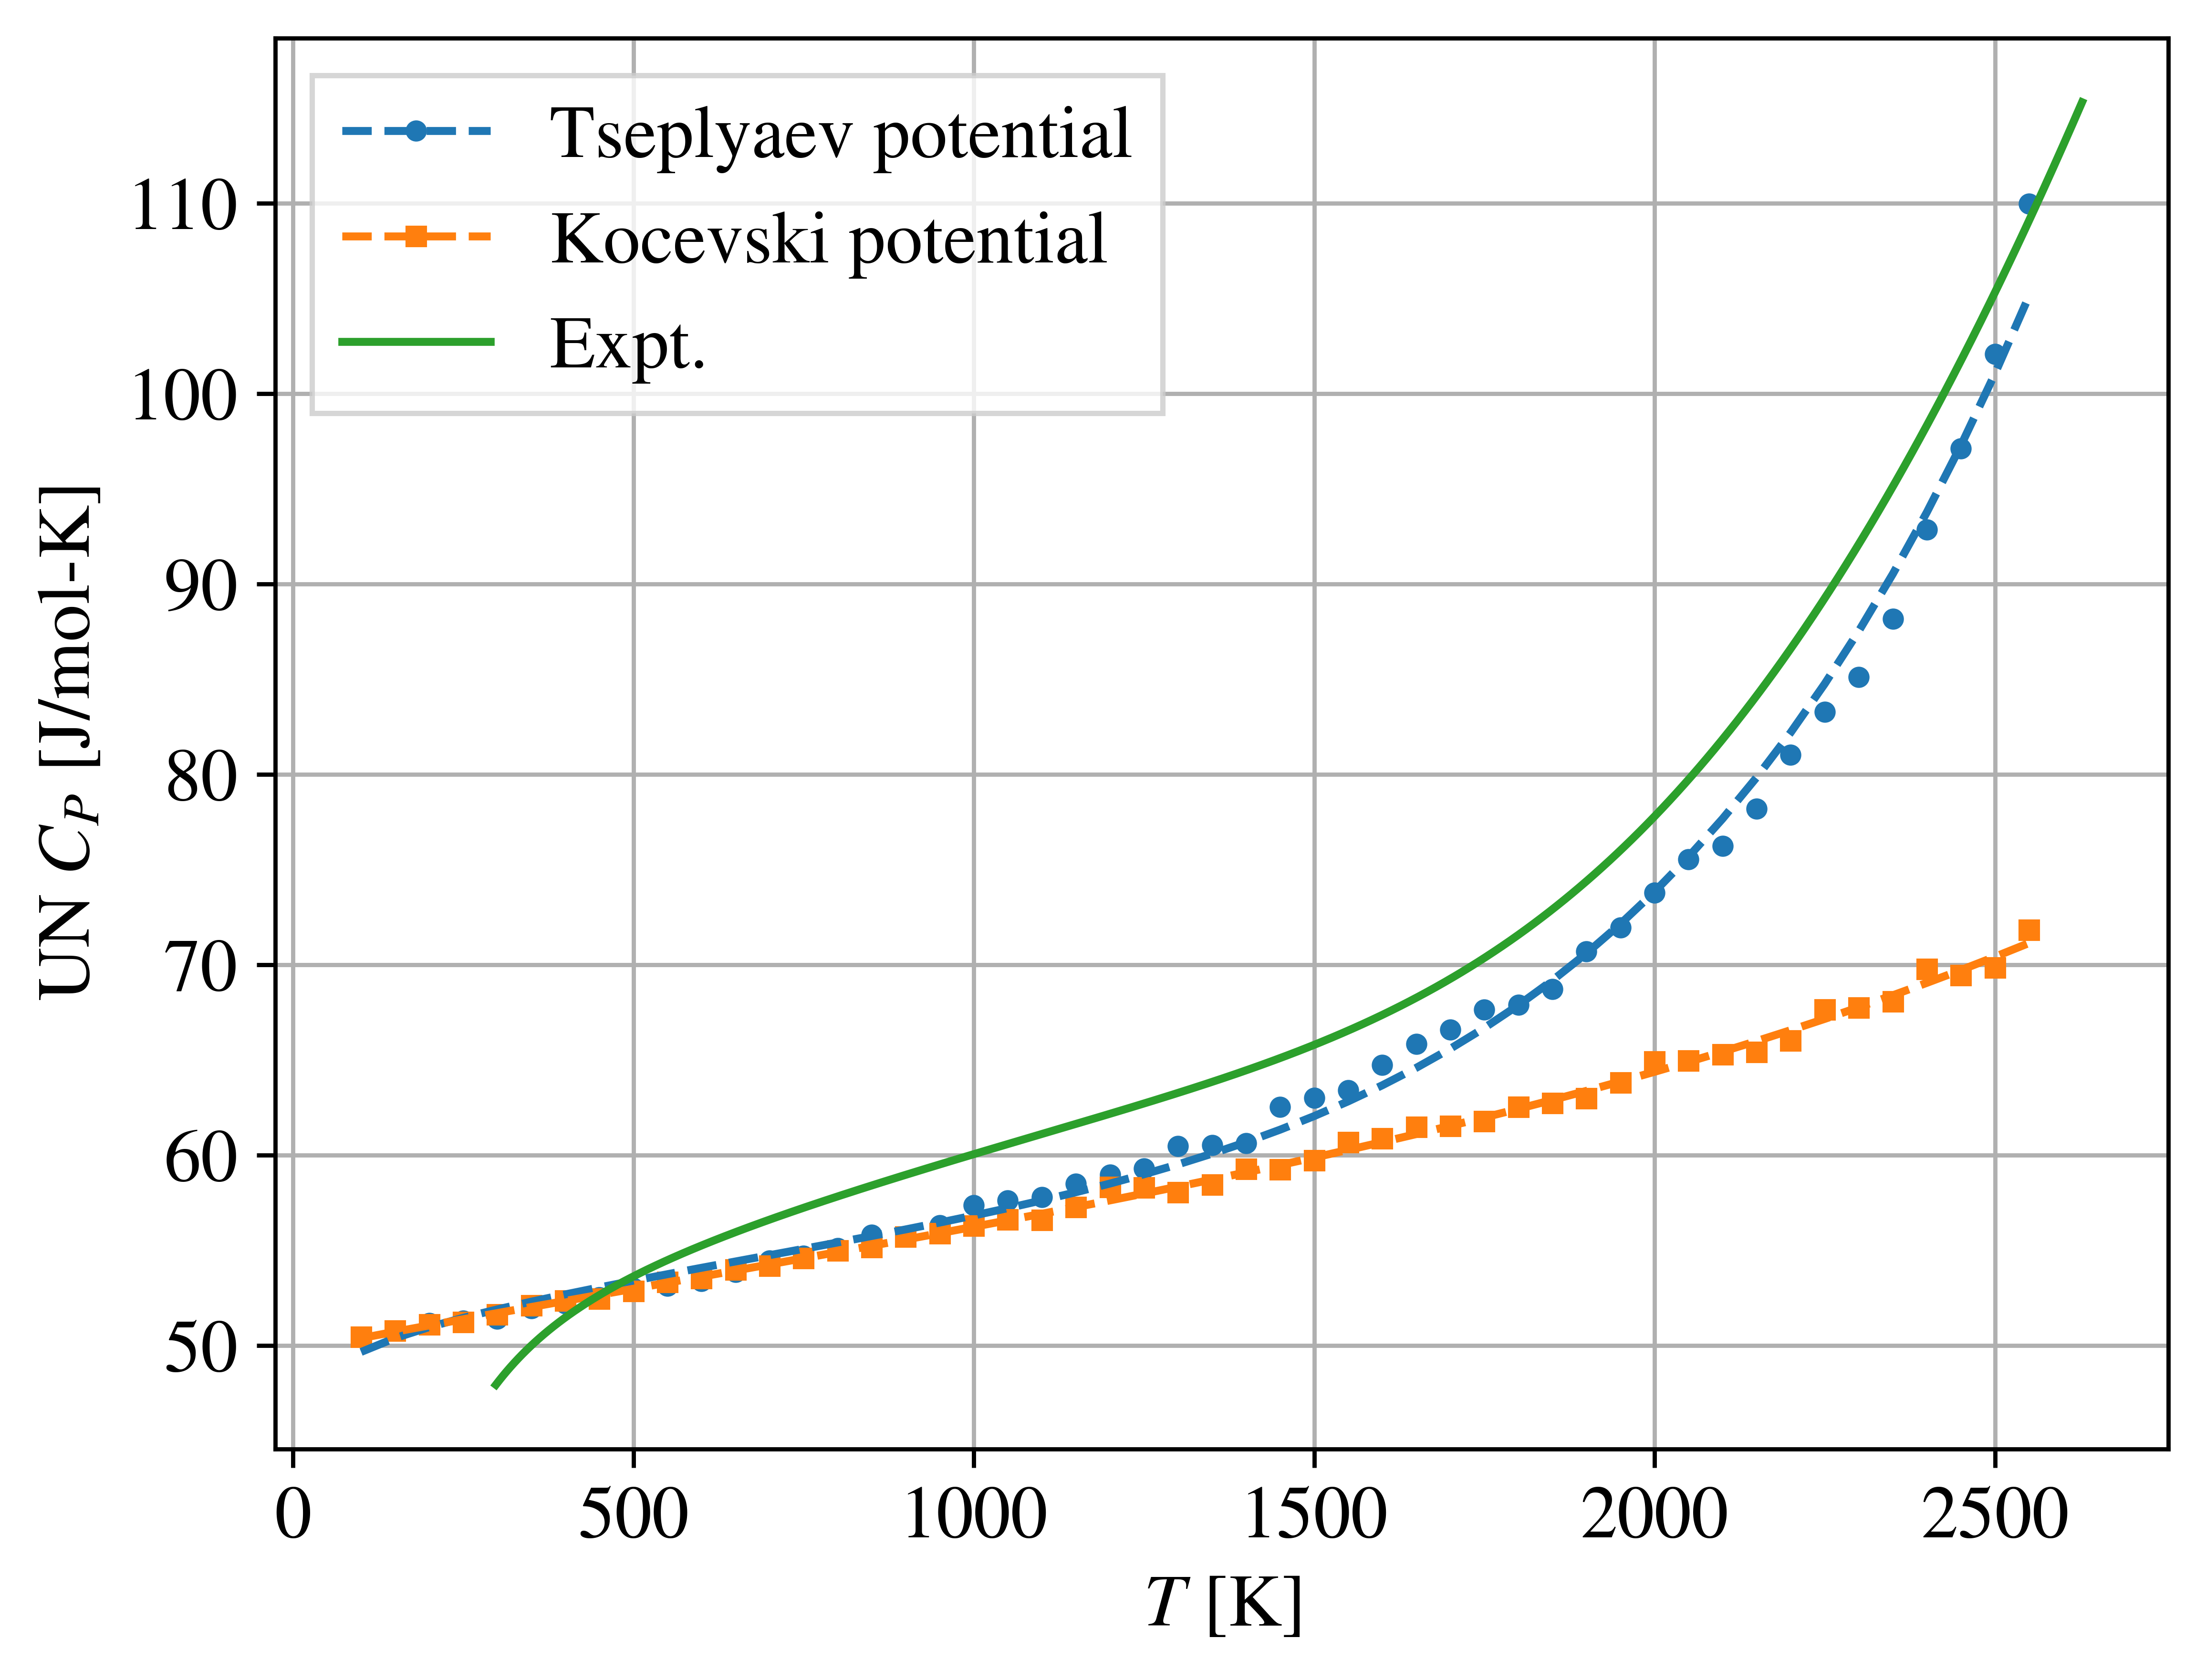
\includegraphics[width=\textwidth]{UNCP.png}
    \caption{}
    \label{Fig:UNCP}
\end{subfigure}
\hfill
\begin{subfigure}{0.45\textwidth}
    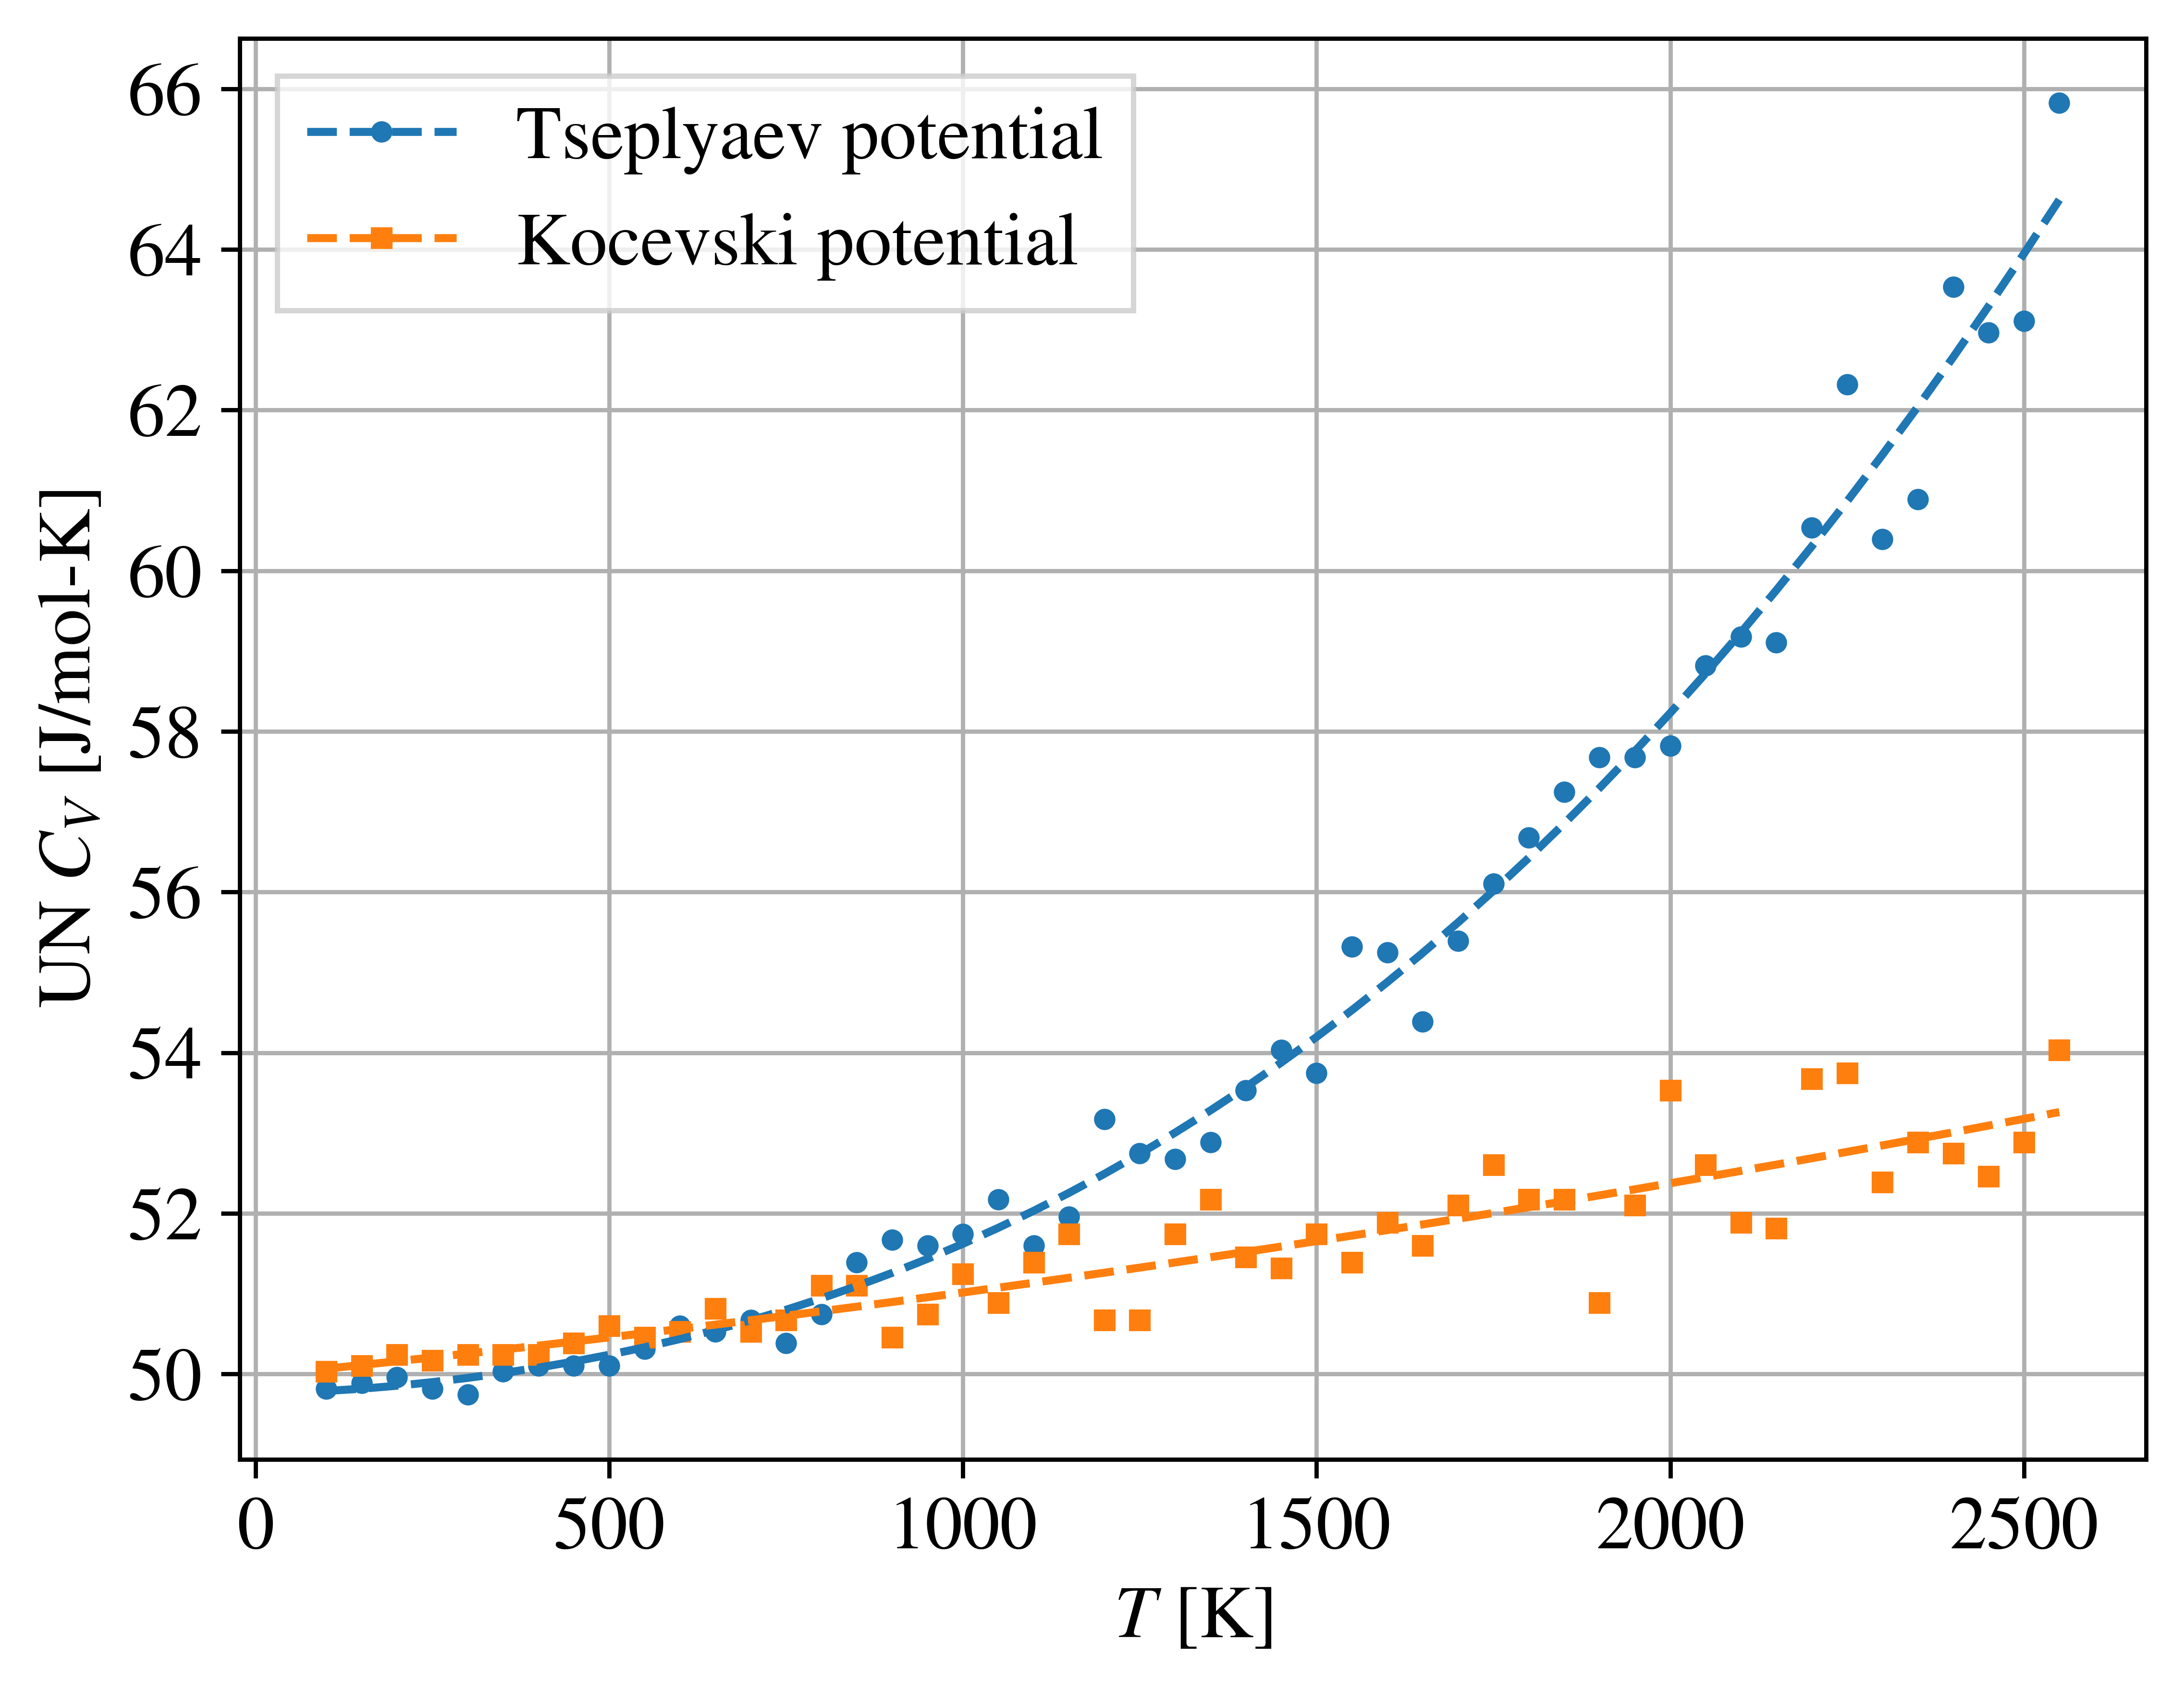
\includegraphics[width=\textwidth]{UNCV.png}
    \caption{}
    \label{Fig:UNCV}
\end{subfigure}
\hfill
\begin{subfigure}{0.45\textwidth}
    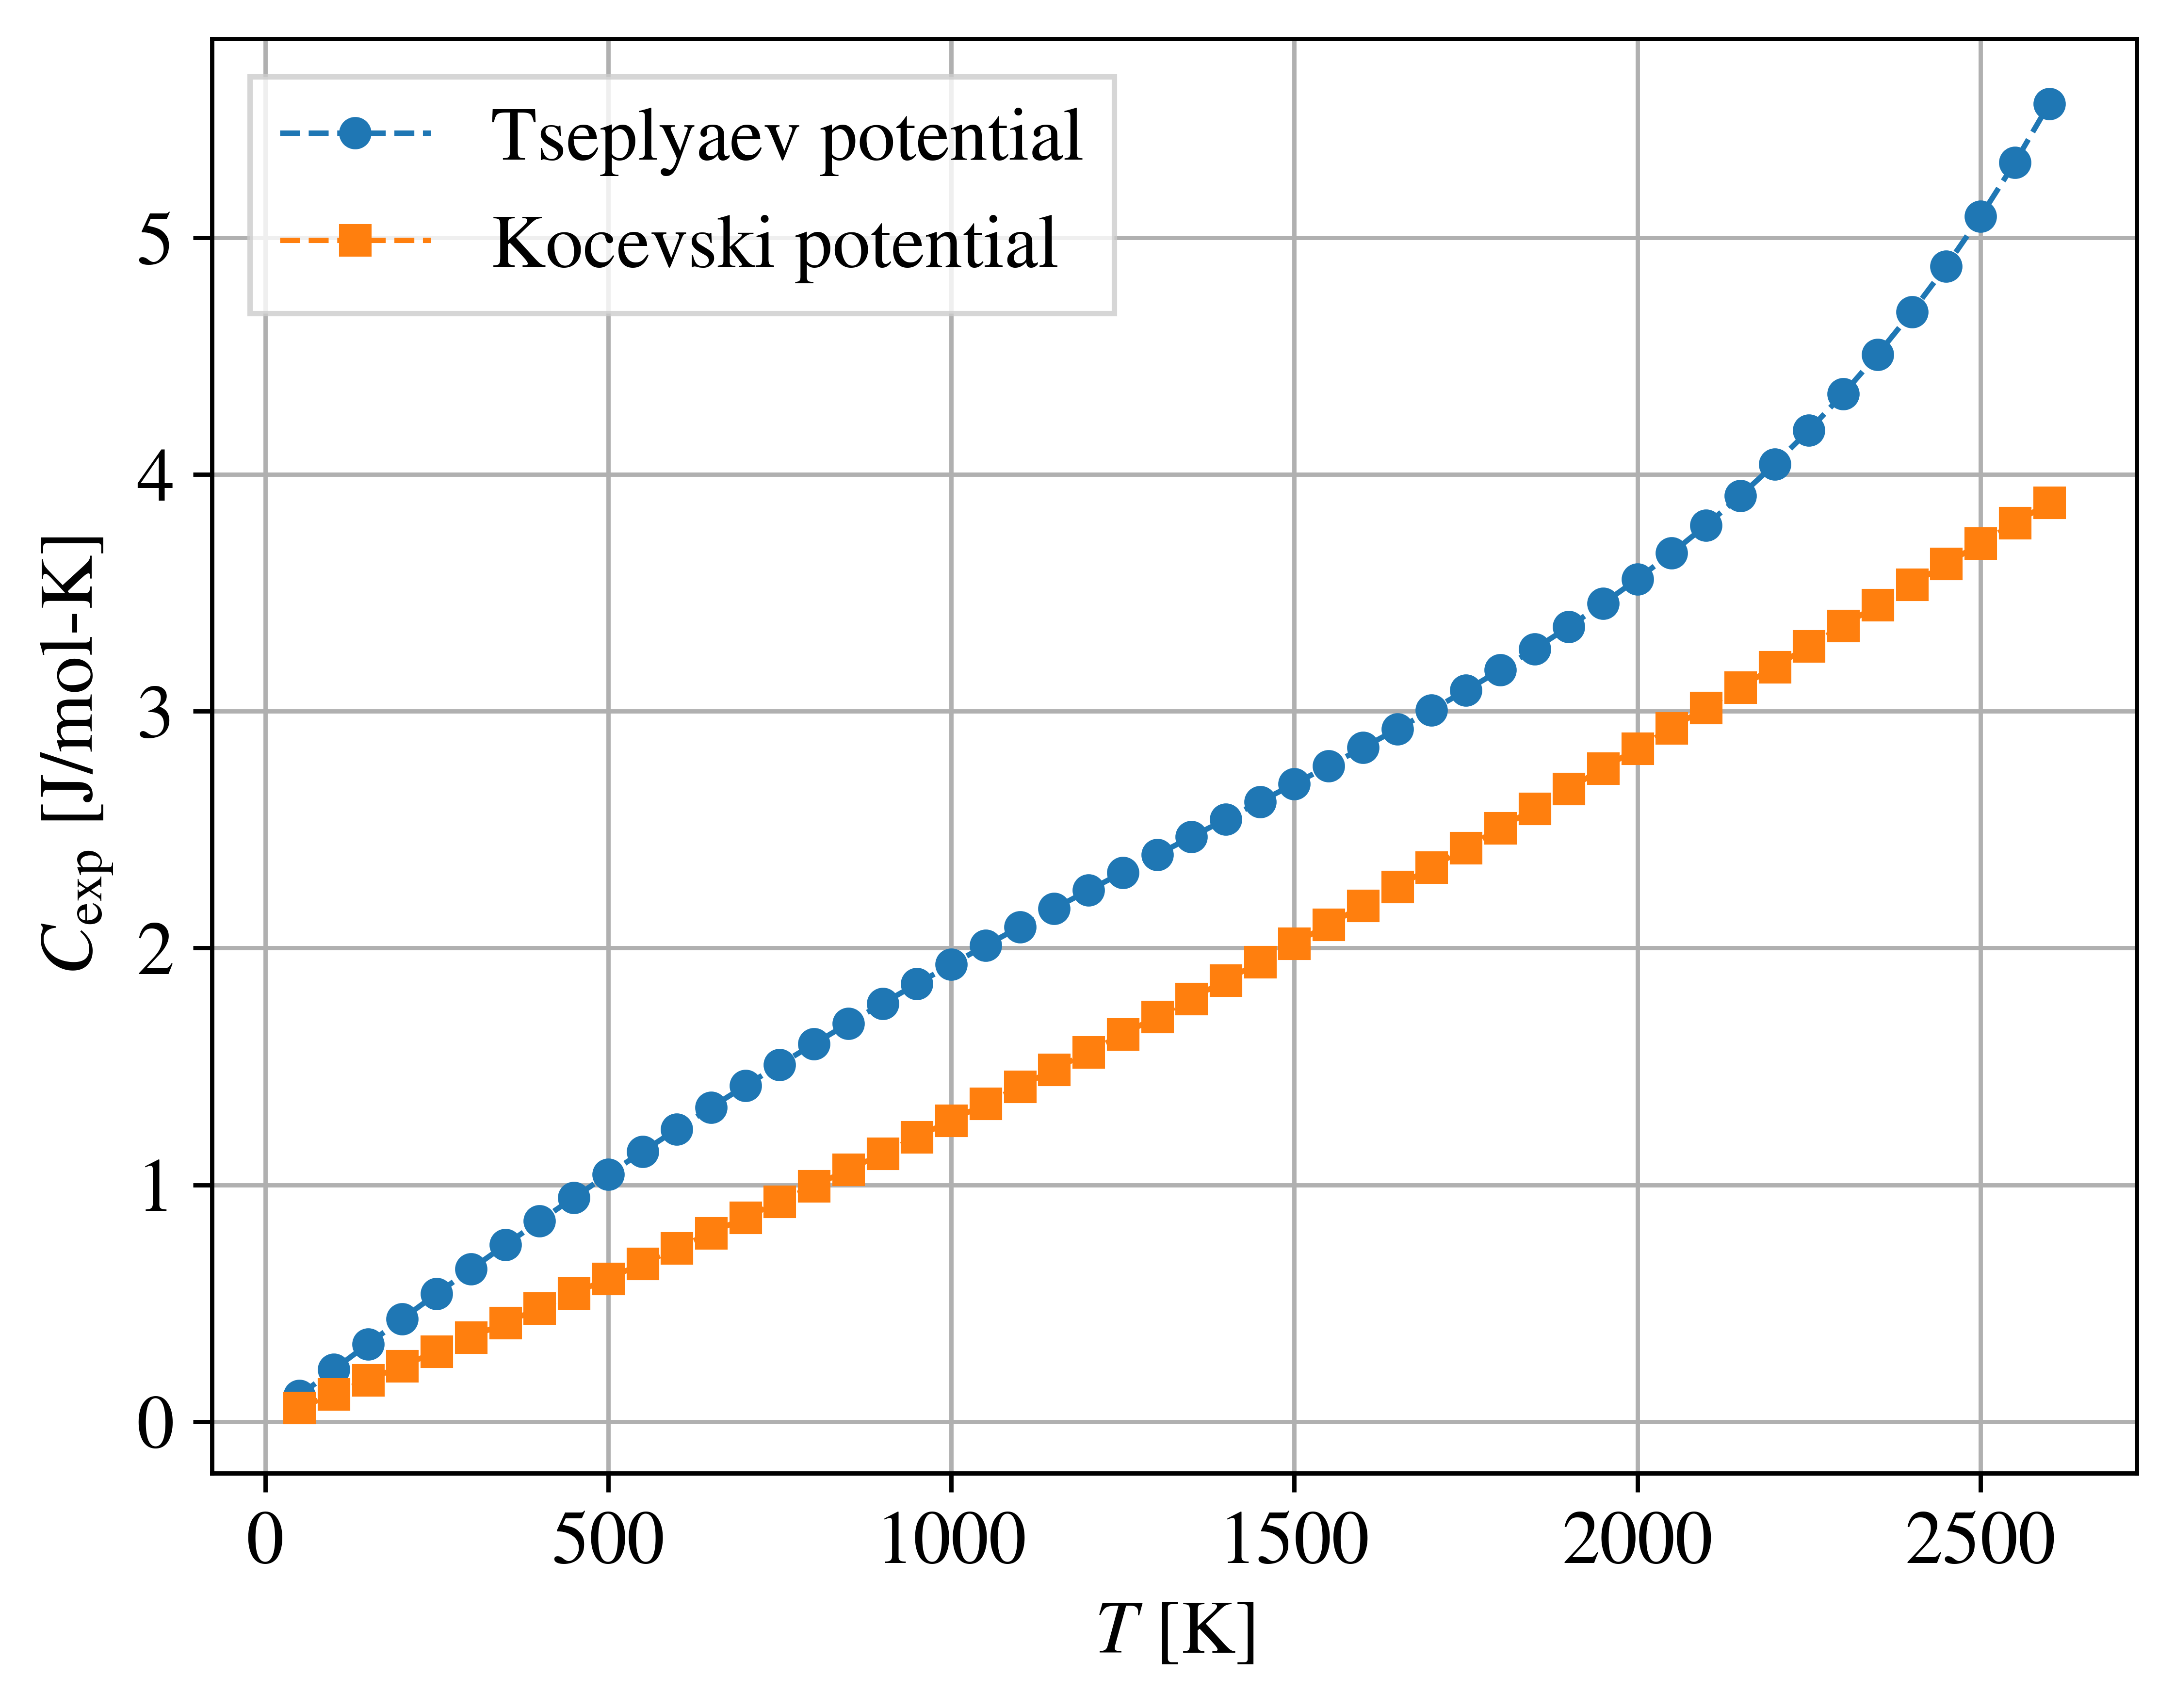
\includegraphics[width=\textwidth]{CD.png}
    \caption{}
    \label{Fig:CD}
\end{subfigure}
\hfill
\begin{subfigure}{0.45\textwidth}
    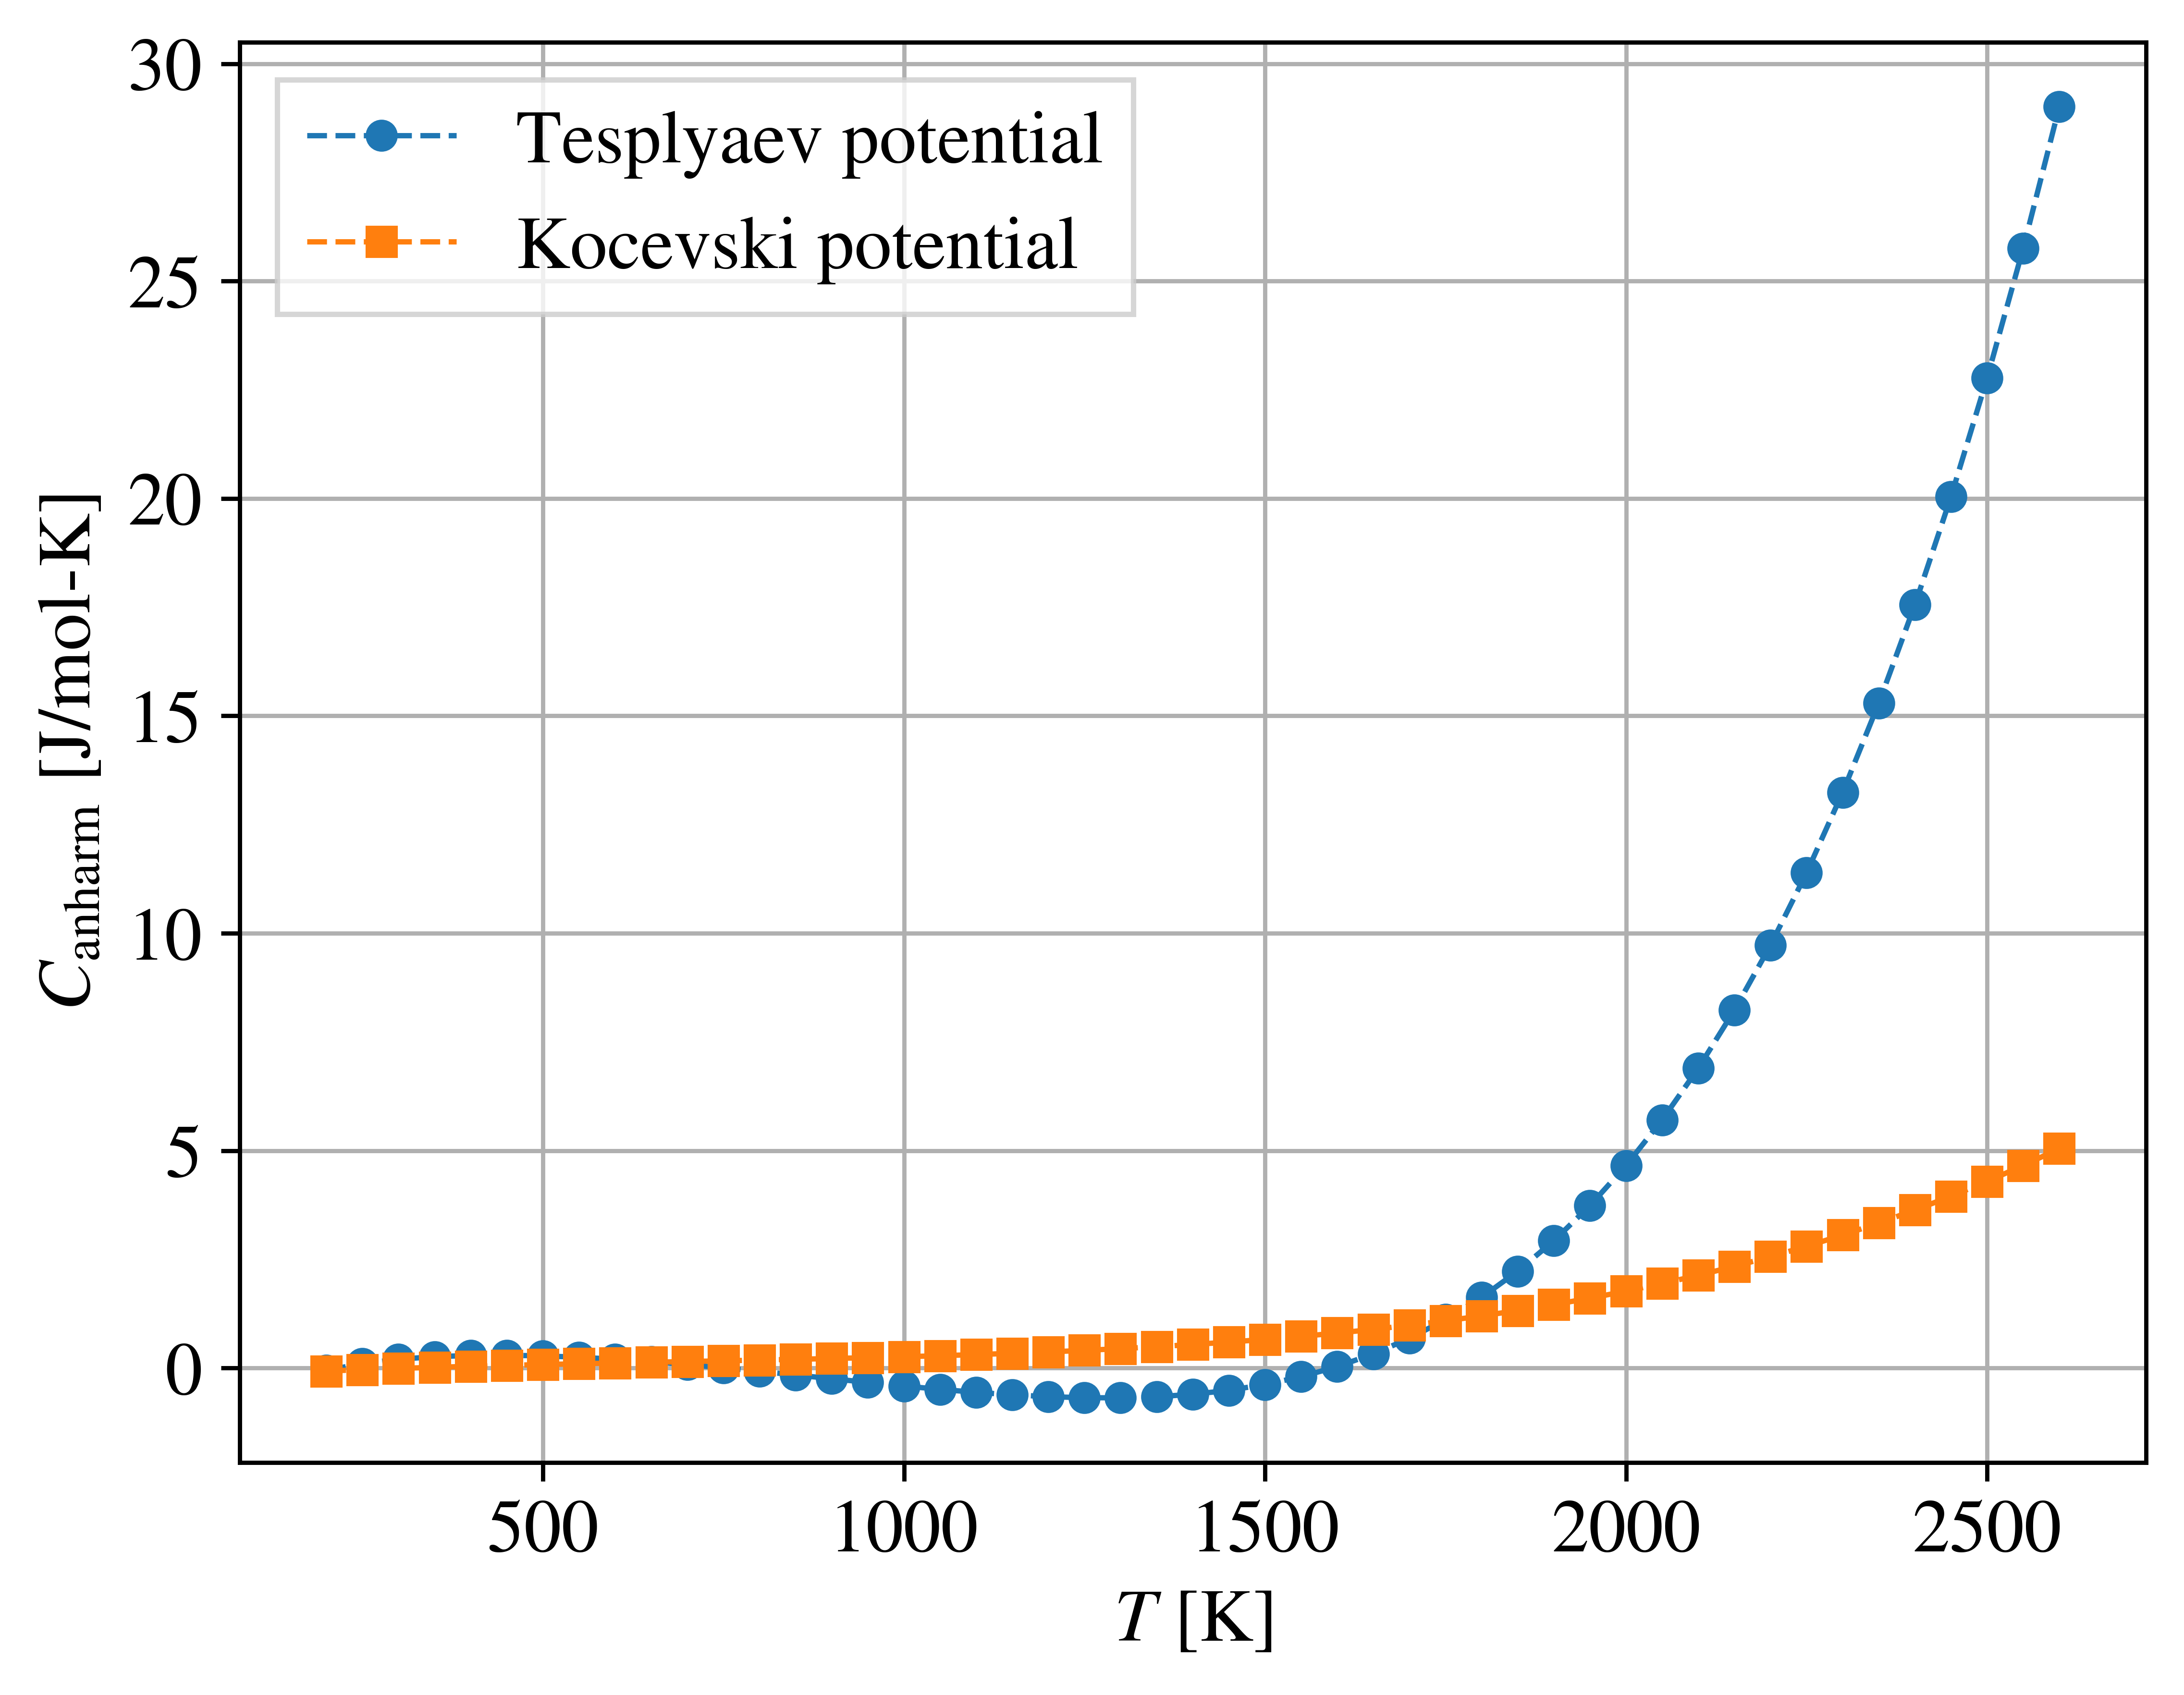
\includegraphics[width=\textwidth]{Canharm.png}
    \caption{}
    \label{Fig:Canharm}
\end{subfigure}
\caption{\textbf{(a)} $C_P$ and \textbf{(b)} $C_V$ of UN as calculated by both potentials and compared to the empirical correlation of Hayes \textit{et al.} (1990) \cite{Hayes1990IV}. \textbf{(c)} The thermal expansion contribution to the specific heat. \textbf{(d)} The anharmonic non-expansive contribution to the specific heat.}
\label{Fig:CVCP}
\end{figure}



\subsection{Phonon properties}
\label{sub:phonon}

The results for the UN phonon properties are shown in \cref{Fig:Phonons}. Experimental data for UN phonon band structure and density of states (DOS) were measured by Jackman \textit{et al.} \cite{Jackman1986} and Aczel \textit{et al.} \cite{Aczel2012} at temperatures of 4.2 K and 5 K, respectively. Given that anharmonicity should be negligible at these cryogenic temperatures, we have carried out phonon calculations in the harmonic approximation for comparison. It can be observed from the phonon band structure (\cref{Fig:PBS}) and phonon DOS (\cref{Fig:PDOS}) that both potentials show a good qualitative agreement with the experimentally observed acoustic phonon spectrum while overestimating the acoustic phonon DOS. It can also be seen in \cref{Fig:PBS} that the Tseplyaev potential only predicts the upper portion of the optical phonon spectrum with moderate qualitative agreement, whereas it completely misses the lower optical branches. The optical branches predicted by the Tseplyaev potential coincide only for some portion of the $k$-path because the potential lacks the long-range electrostatic interaction, which is responsible for splitting the longitudinal and transverse optical phonon branches in ionic materials \cite{Zhou2009}. \cref{Fig:PDOS} shows that the optical phonon frequency range predicted by the Kocevski potential is overestimated by about 1.9 THz compared to experimental measurements, incorrectly describing all optical branches.

\begin{figure}[h!]
\centering
\begin{subfigure}{0.45\textwidth}
    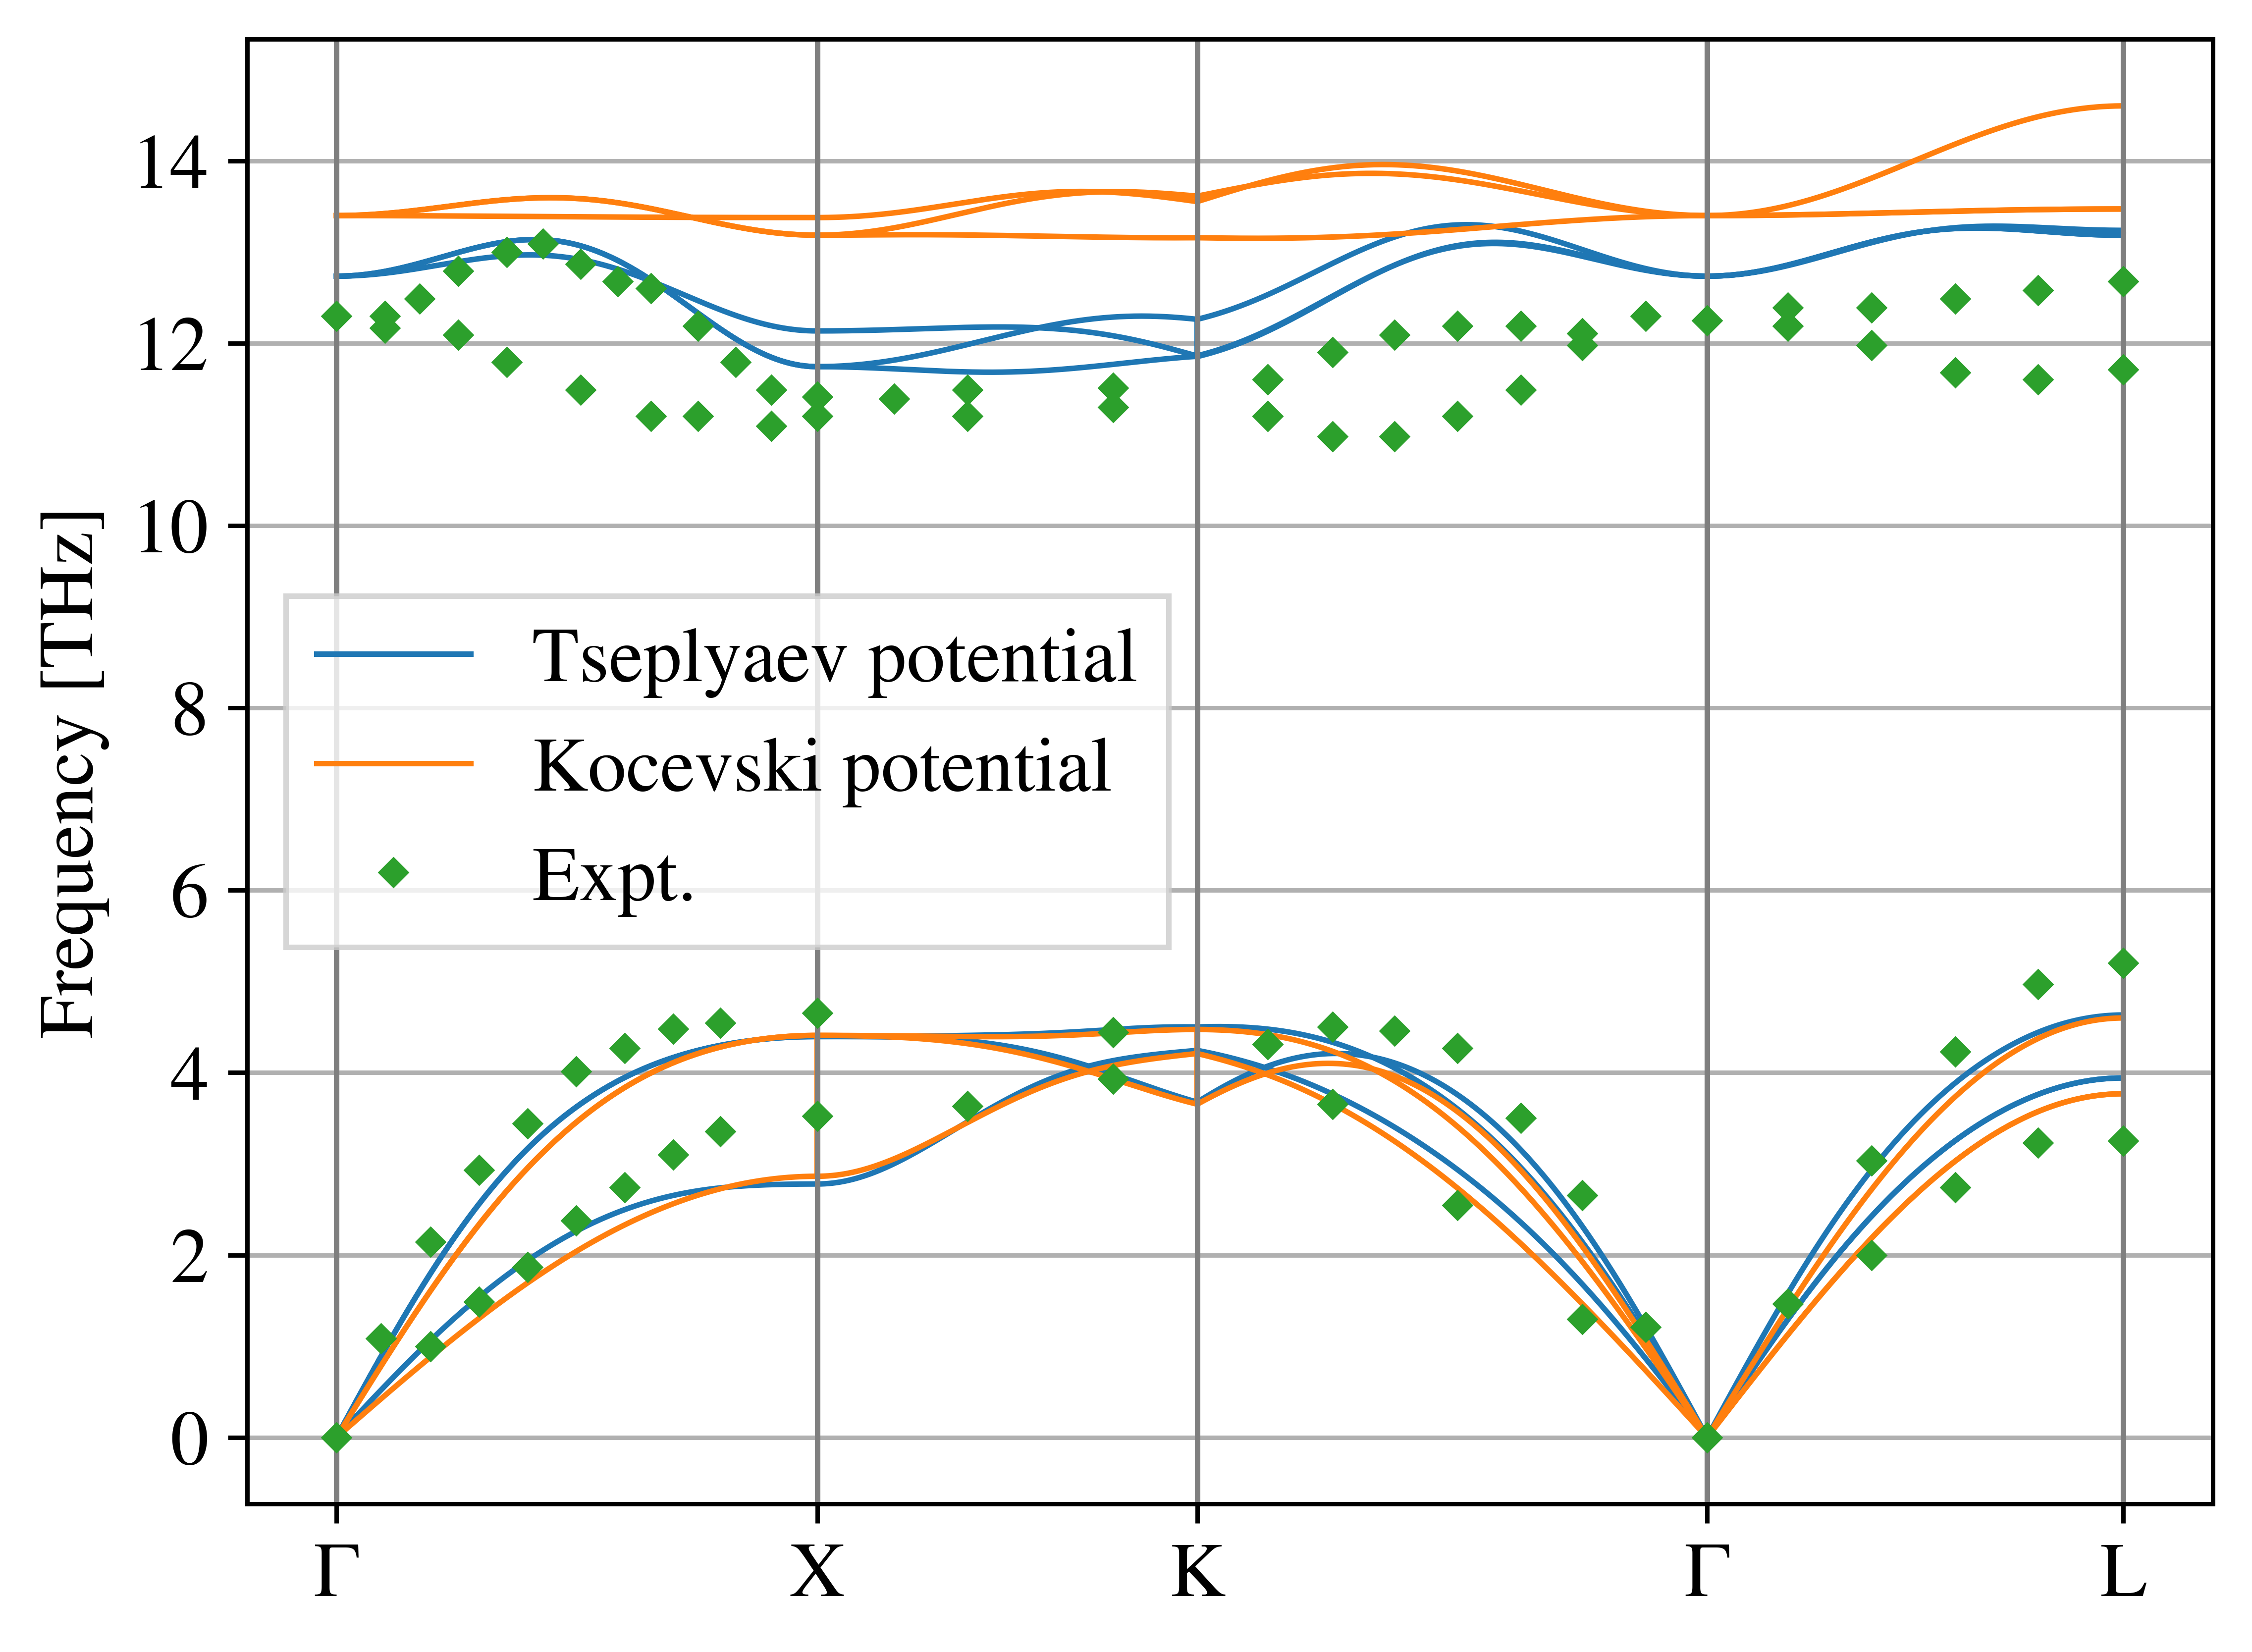
\includegraphics[width=\textwidth]{PBS.png}
    \caption{}
    \label{Fig:PBS}
\end{subfigure}
\hfill
\begin{subfigure}{0.45\textwidth}
    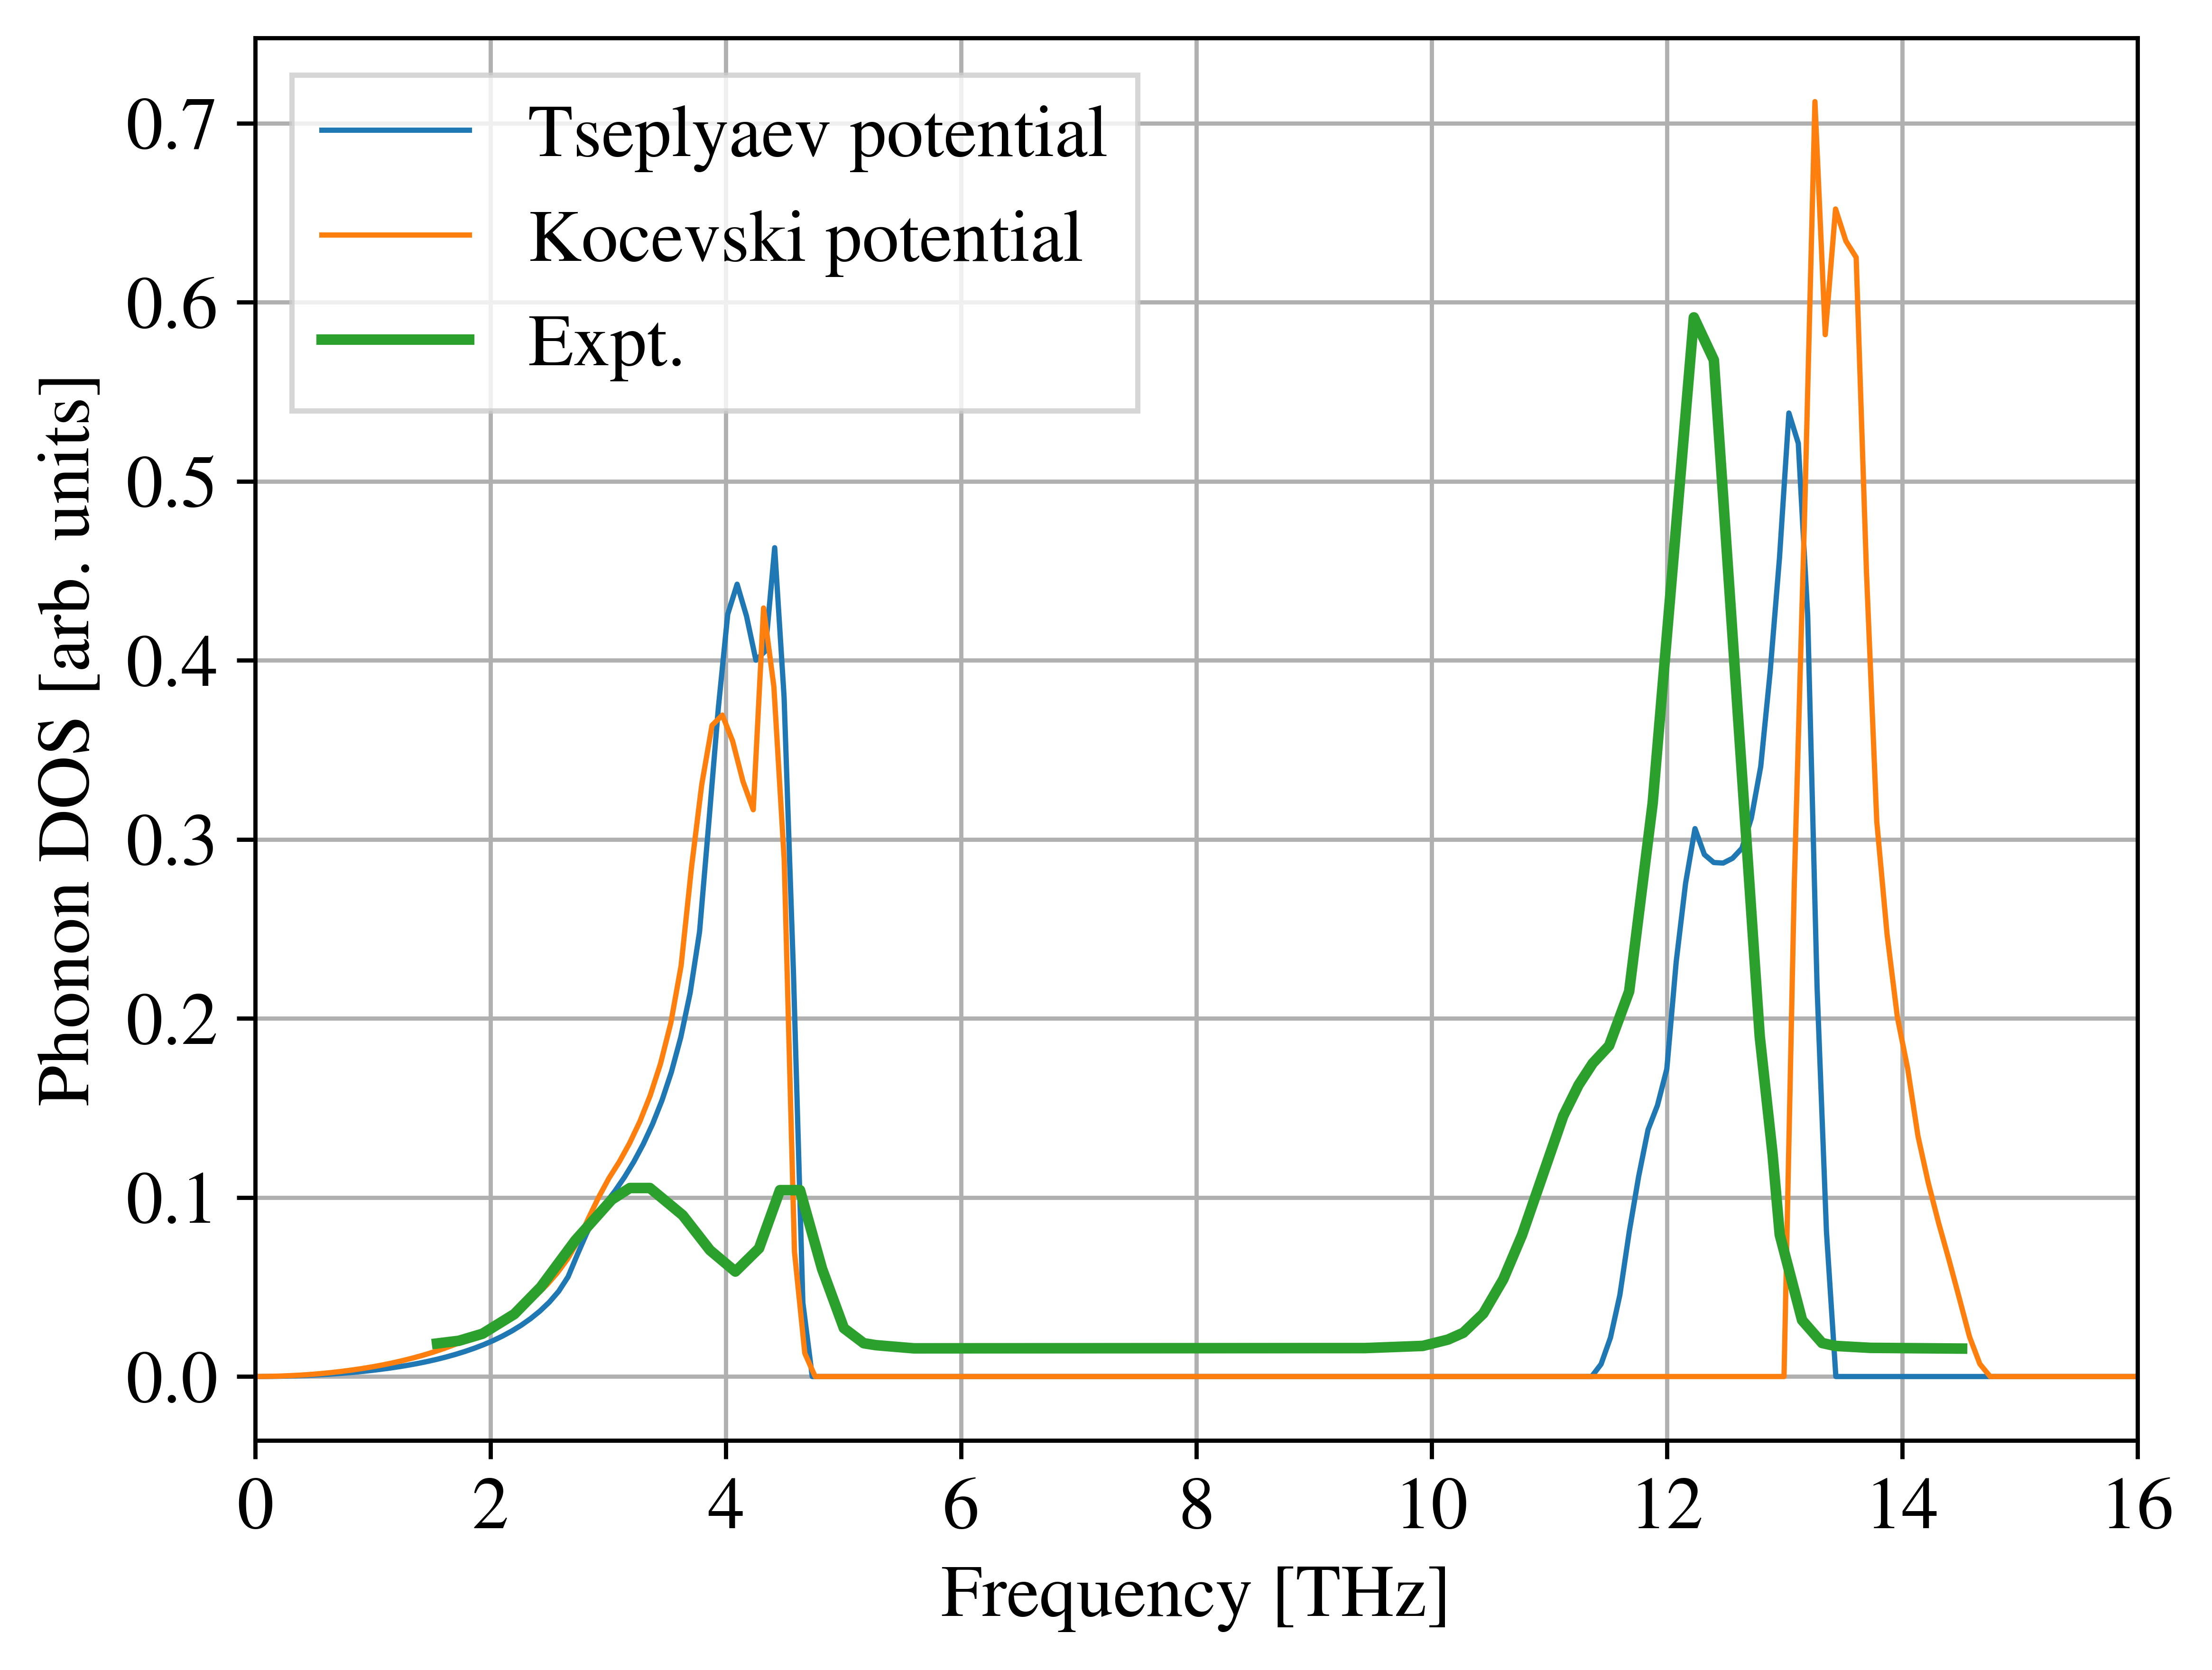
\includegraphics[width=\textwidth]{PDOS.png}
    \caption{}
    \label{Fig:PDOS}
\end{subfigure}
\caption{\textbf{(a)} UN phonon band structure as calculated by both potentials and compared to the experimental data of Jackman \textit{et al.} \cite{Jackman1986}. \textbf{(b)} UN phonon density of states (DOS) as calculated by both potentials and compared to the inelastic neutron scattering data of Aczel \textit{et al.} \cite{Aczel2012}. The areas under the phonon DOS plots have been normalized to 1 to allow comparison between calculations and the experiment.}
\label{Fig:Phonons}
\end{figure}

The acoustic phonon spectrum and low-frequency DOS are related to the vibrations of the heavier uranium atoms, whereas the optical phonon spectrum and high-frequency DOS are related to the vibrations of the lighter nitrogen atoms \cite{Baranov2013, Boer2018}. Therefore, it can be concluded that both potentials accurately model the uranium atom vibrations whereas only the Tseplyaev potential can qualitatively model the nitrogen atom vibrations. From these results, the Kocevski potential underestimation of the UN $C_P$ compared to that predicted by the Tseplyaev potential can be attributed to the Kocevski potential overestimation of the optical phonon frequency range. The contribution of the optical phonons to the specific heat can be treated by the Einstein model. Due to their nearly flat dispersion curve, optical phonons are approximated within the Einstein model as having a single average frequency, $\omega_E$, independent of $k$. From the experimental UN dispersion curve, $\omega_E$ = 12.0 THz, whereas $\omega_E$ = 12.5 THz for the Tseplyaev potential, and $\omega_E$ = 13.9 THz for the Kocevski potential. Because phonons are bosons, they follow the Bose-Einstein distribution \cite{Boer2018}:
\begin{equation}
f_{BE} = \frac{1}{\mathrm{exp} \left( \hbar \omega / k_B T \right)-1}
\label{Eq:Bose}
\end{equation}
where $f_{BE}$ quantifies the mean number of phonons of frequency $\omega$ present in thermal equilibrium at temperature $T$ \cite{Ashcroft1976}. With the Kocevski potential overestimating $\omega_E$, it predicts a smaller average number of excited optical phonons, which leads to a smaller contribution of the optical phonons to the UN specific heat. Torres \textit{et al.} \cite{Torres2020} also observed the same trend while analyzing the phonon properties predicted by existing \ce{UO2} empirical potentials. By including both harmonic and higher-order force constants in their phonon calculations, they found that \ce{UO2} empirical potentials that overestimate the 0 K optical phonon frequency range tend to underestimate the specific heat, especially at near-melting temperatures. Zhou \textit{et al.} \cite{Zhou2009} also made a similar observation about the Stillinger-Weber potential of GaN, and attributed its underestimation of the specific heat at high temperatures to the overestimated optical phonon range. The Debye temperature quantifies the temperature above which all phonon modes become excited and below which some phonon modes freeze out \cite{Ashcroft1976}. Based on our analysis in \cref{Sec:Elastic}, $\theta_D$ is around 362 K, which means that even at temperatures near RT we can expect optical phonons to contribute to the UN specific heat. Baranov \textit{et al.} \cite{Baranov2013} also noted that due to the ionic character of the UN chemical bond, optical phonons are expected to predominate the oscillation spectrum of the UN lattice at temperatures above $\theta_D$.

The agreement between the lattice thermal conductivity predicted by Galvin \textit{et al.} \cite{Galvin2023} using both potentials despite the discrepancy of the predicted specific heats can be understood if we note that the two potentials predict the same acoustic phonon spectrum and DOS at 0 K. For bulk materials, the thermal conductivity is largely dictated by acoustic phonons because they are the main heat carriers \cite{Li2020}. In contrast, the contribution of optical phonons to the thermal conductivity of bulk materials is very small due to their short lifetimes and low group velocities \cite{Tian2011}.



\subsection{Point defect formation energies}

Perfect $6 \times 6 \times 6$ supercells of UN were energy-minimized at 0 K using the conjugate gradient algorithm implemented in LAMMPS. A fractional energy tolerance of $1 \times 10^{-9}$ was used allowing volume change. For the Tseplyaev potential, we used energy tolerances in the range $10^{-6}$-$10^{-15}$ and found that the raw formation energies of the defective supercells vary by several eV with decreasing the energy tolerance down to a tolerance of $10^{-9}$ at which the raw formation energy becomes somewhat insensitive to the energy tolerance. This is indicative of the complex potential energy surface predicted by the Tseplyaev potential and the likely existence of several metastable states. This strong dependence of the raw formation energy on energy tolerance was not observed for the Kocevski potential. The cohesive energies of UN, $\alpha$-U, and \ce{UN2} and chemical potentials were calculated for both potentials and are shown in \cref{Tab:CohesiveE,Tab:ChemPot}. It should be noted that the Kocevski potential predicts positive cohesive energy for $\alpha$-U (i.e., it cannot predict a stable $\alpha$-U phase), which would lead to unphysical chemical potentials and incorrect formation energies for the U-rich and stoichiometric conditions. For this reason, point defects under U-rich and stoichiometric conditions are not considered for the Kocevski potential in this work. 

For the 0 K calculations, point defects were then introduced into $6 \times 6 \times 6$ UN supercells. U and N interstitials were inserted only in cubic interstitial sites. Yang and Kaltsoyannis \cite{Yang2021} have observed that when a U Frenkel defect is introduced within a UN supercell, it is annihilated by the tiny atomic movements of the relaxation process. To prevent this phenomenon, the initial forces on all inserted interstitials were set to zero. Defective supercells were relaxed using the same procedure used for the perfect supercells.

To avoid the possibility of defective supercells converging to metastable energy states by static minimization at 0 K, the 0 K formation energies are averaged over many defect configurations, and, additionally, the formation energies are also calculated at 1 K. $8 \times 8 \times 8$ supercells of UN are equilibrated in the \textit{NPT} ensemble for 50 ps, where the system's potential energy is averaged over the last 20 ps. Point defects are inserted in the equilibrated UN supercells, and the defective system is allowed to evolve under the \textit{NPT} ensemble for 50 ps where the system's potential energy is also averaged over the last 20 ps. The calculation is repeated using five unique initial velocity distributions, utilizing the average potential energy of this sample to obtain defect energetics. Chemical potentials and formation energies are calculated using the same procedure employed at 0 K. The Tseplyaev potential is also used to calculate the finite-temperature formation enthalpy for U FD, N FD, and SD with 15 unique initial velocity distributions in the temperature range of 100-1500 K. The 1500 K limit is chosen because in UN diffusion begins to be experimentally observed at this temperature \cite{Hayes1990III}. Thus, at and beyond 1500 K, the measured raw formation enthalpies would be affected by defect migration.

\begin{table}[h!]
    \centering
    \footnotesize
    \caption{Formation energies (eV) for stoichiometric point defects. FD stands for Frenkel defect, and SD stands for Schottky defect. A semi-bonded SD is composed of two vacancies at $(0, 0, 0)$ and $(0.5, 0.5, 0.5)$.}
    \label{Tab:StoicDef}
    \begin{tabular}{l|cc|cc|c}
    \hline
                & \multicolumn{2}{c|}{Tseplyaev potential}            & \multicolumn{2}{c|}{Kocevski potential}  & \multirow{2}{*}{DFT} \\
& 0 K & 1 K & 0 K & 1 K & \\
\hline
Unbonded U FD            & 9.32   & 8.02            & 14.41  & 14.30 & 9.46 \cite{Yang2021}, 6.31-10.19 \cite{Kocevski2022I} \\
Bonded U FD              & 7.26   & -               & 10.3   & -     & - \\
Unbonded N FD            & 4.67   & 4.50            & 4.03   & 4.00  & 4.90-5.04 \cite{Yang2021}, 4.43-4.95 \cite{Kocevski2022I} \\
Bonded N FD              & 3.76   & -               & 3.23   & -     & - \\
Unbonded SD              & 4.57   & 4.52            & 3.98   & 3.88  & 4.96-5.15 \cite{Yang2021}, 4.25-5.47 \cite{Kocevski2022I} \\
Semi-bonded SD           & 4.51   & -               & 3.99   & -     & - \\
Bonded SD (divacancy)    & 4.35   & -               & 3.04   & -     & 4.17 \cite{Yang2021} \\
    \hline
    \end{tabular}
\end{table}

\begin{table}[h!]
\tiny 
\centering
\caption{Formation energies (eV) for non-stoichiometric point defects. Standard Kröger-Vink notation \cite{Kroger1956} has been used for point defects but with charges omitted due to the inability of MD to simulate charged defects.}
\begin{tabular}{l|cc|c|cc|c|cc|cc|c}
\hline
& \multicolumn{3}{c|}{U-rich} & \multicolumn{3}{c|}{Stoichiometric} & \multicolumn{5}{c}{N-rich} \\
\hline
& \multicolumn{2}{c|}{Tseplyaev} & \multirow{2}{*}{DFT} & \multicolumn{2}{c|}{Tseplyaev} & \multirow{2}{*}{DFT} & \multicolumn{2}{c|}{Tseplyaev} & \multicolumn{2}{c|}{Kocevski} & \multirow{2}{*}{DFT} \\
& 0 K & 1 K                &                      & 0 K & 1 K                &                      & 0 K & 1 K                & 0 K & 1 K & \\  
\hline
$V_U$ & 3.45            & 3.33            & 3.17-3.43 \cite{Yang2021}, 3.27-3.86  \cite{Kocevski2022I} & 2.19            & 2.14            & 2.75-3.01 \cite{Yang2021} & 0.93            & 0.95            & 0.60             & 0.54  & 2.34-2.60 \cite{Yang2021}, 2.09-2.58  \cite{Kocevski2022I} \\
$V_N$ & 1.11            & 1.29            & 1.76-1.90 \cite{Yang2021}, 0.62-1.86  \cite{Kocevski2022I} & 2.37            & 2.48            & 2.18-2.31 \cite{Yang2021} & 3.62            & 3.67            & 3.35             & 3.34  & 2.59-2.72 \cite{Yang2021}, 1.42-2.82  \cite{Kocevski2022I} \\
$U_i$ & 6.43            & 3.99            & 2.81-6.33 \cite{Kocevski2022I}                             & 7.69            & 5.18            & -                         & 8.95            & 6.37            & 13.82            & 13.76 & 3.79-7.78  \cite{Kocevski2022I} \\
$N_i$ & 3.73            & 3.21            & 2.96-3.82 \cite{Kocevski2022I}                             & 2.47            & 2.02            & -                         & 1.21            & 0.83            & 0.89             & 0.66  & 2.00-3.01  \cite{Kocevski2022I} \\
$U_N$ & 1.61            & 1.86            & 1.74-3.16 \cite{Kocevski2022I}                             & 4.13            & 4.24            & -                         & 6.65            & 6.62            & 18.32            & 15.90 & 3.72-5.52  \cite{Kocevski2022I} \\
$N_U$ & 9.32            & 5.84            & 5.99-7.67 \cite{Kocevski2022I}                             & 6.80            & 3.46            & -                         & 4.28            & 1.08            & 4.71             & 1.70  & 4.06-5.19  \cite{Kocevski2022I} \\
\hline
\end{tabular}
\label{Tab:Ef}
\end{table}

The calculated formation energies are reported in \cref{Tab:StoicDef,Tab:Ef}. Bonded SD and FD are formed by introducing the two vacancies, and the vacancy and interstitial, respectively, within the same unit cell, whereas unbonded SD and FD are formed by introducing the two vacancies, and the vacancy and interstitial, respectively, within different unit cells. Dashes in \cref{Tab:StoicDef} for bonded defects at 1 K indicate that these defects relaxed to the defect-free crystal structure. The formation energy of the N FD is slightly higher than the formation energies of the unbonded SD and divacancy due to the lattice's compact structure which offers limited room for an interstitial. The formation energies predicted by the Tseplyaev potential at 0 K and 1 K are generally consistent with each other except for the values predicted for unbonded U FD, $U_i$, and $N_U$ which show differences in the range 1.30-3.48 eV, with the 0 K values being generally larger than the 1 K values. This is because calculating the formation energies at 1 K using the Tseplyaev potential allows us to approach the ground state of the defect structure, whereas the calculation at 0 K fails to do so. This is especially true for $U_i$, whose most stable configuration in UN is reported as the dumbbell configuration \cite{Kuksin2016}, whereas, by visual inspection of the $U_i$ structure at 0 K (not shown), $U_i$ still resides at the cubic interstitial site after static minimization using the Tseplyaev potential. The difference in $U_i$ formation energy between 0 K and 1 K also explains the difference in the formation energy of U FD. This discrepancy most likely signifies that the Tseplyaev potential predicts metastable states for the defected UN supercells at 0 K, a situation that we also encountered with strained UN supercells at 0 K. Thus, caution should be exercised when utilizing or examining 0 K defect properties calculated by the Tseplyaev potential. The formation energies predicted by the Tseplyaev potential generally show excellent agreement with the DFT-predicted values for U-rich, N-rich, and stoichiometric conditions. The Kocevski potential predicts formation energies for N FD and SD in agreement with DFT, but it overestimates the U FD defect by more than 4 eV. As explained previously, the Kocevski potential cannot predict formation energies for U-rich and stoichiometric conditions due to the inability to describe metallic U. However, for N-rich conditions, the formation energies predicted by the Kocevski potential qualitatively agree with DFT-values for most defects except for $U_i$ and $U_N$, which are overestimated by a factor of 2-3. It can be concluded that the Tseplyaev potential shows a better performance in the calculation of point defect formation energy, whereas the Kocevski potential is only suitable for stoichiometric point defects. It can also be concluded that in U-rich conditions, $V_N$ and $U_N$ accommodate most of the off-stoichiometry, whereas, in N-rich conditions, $V_U$ and $N_i$ accommodate most of the off-stoichiometry.

\begin{figure}[h!]
    \centering
    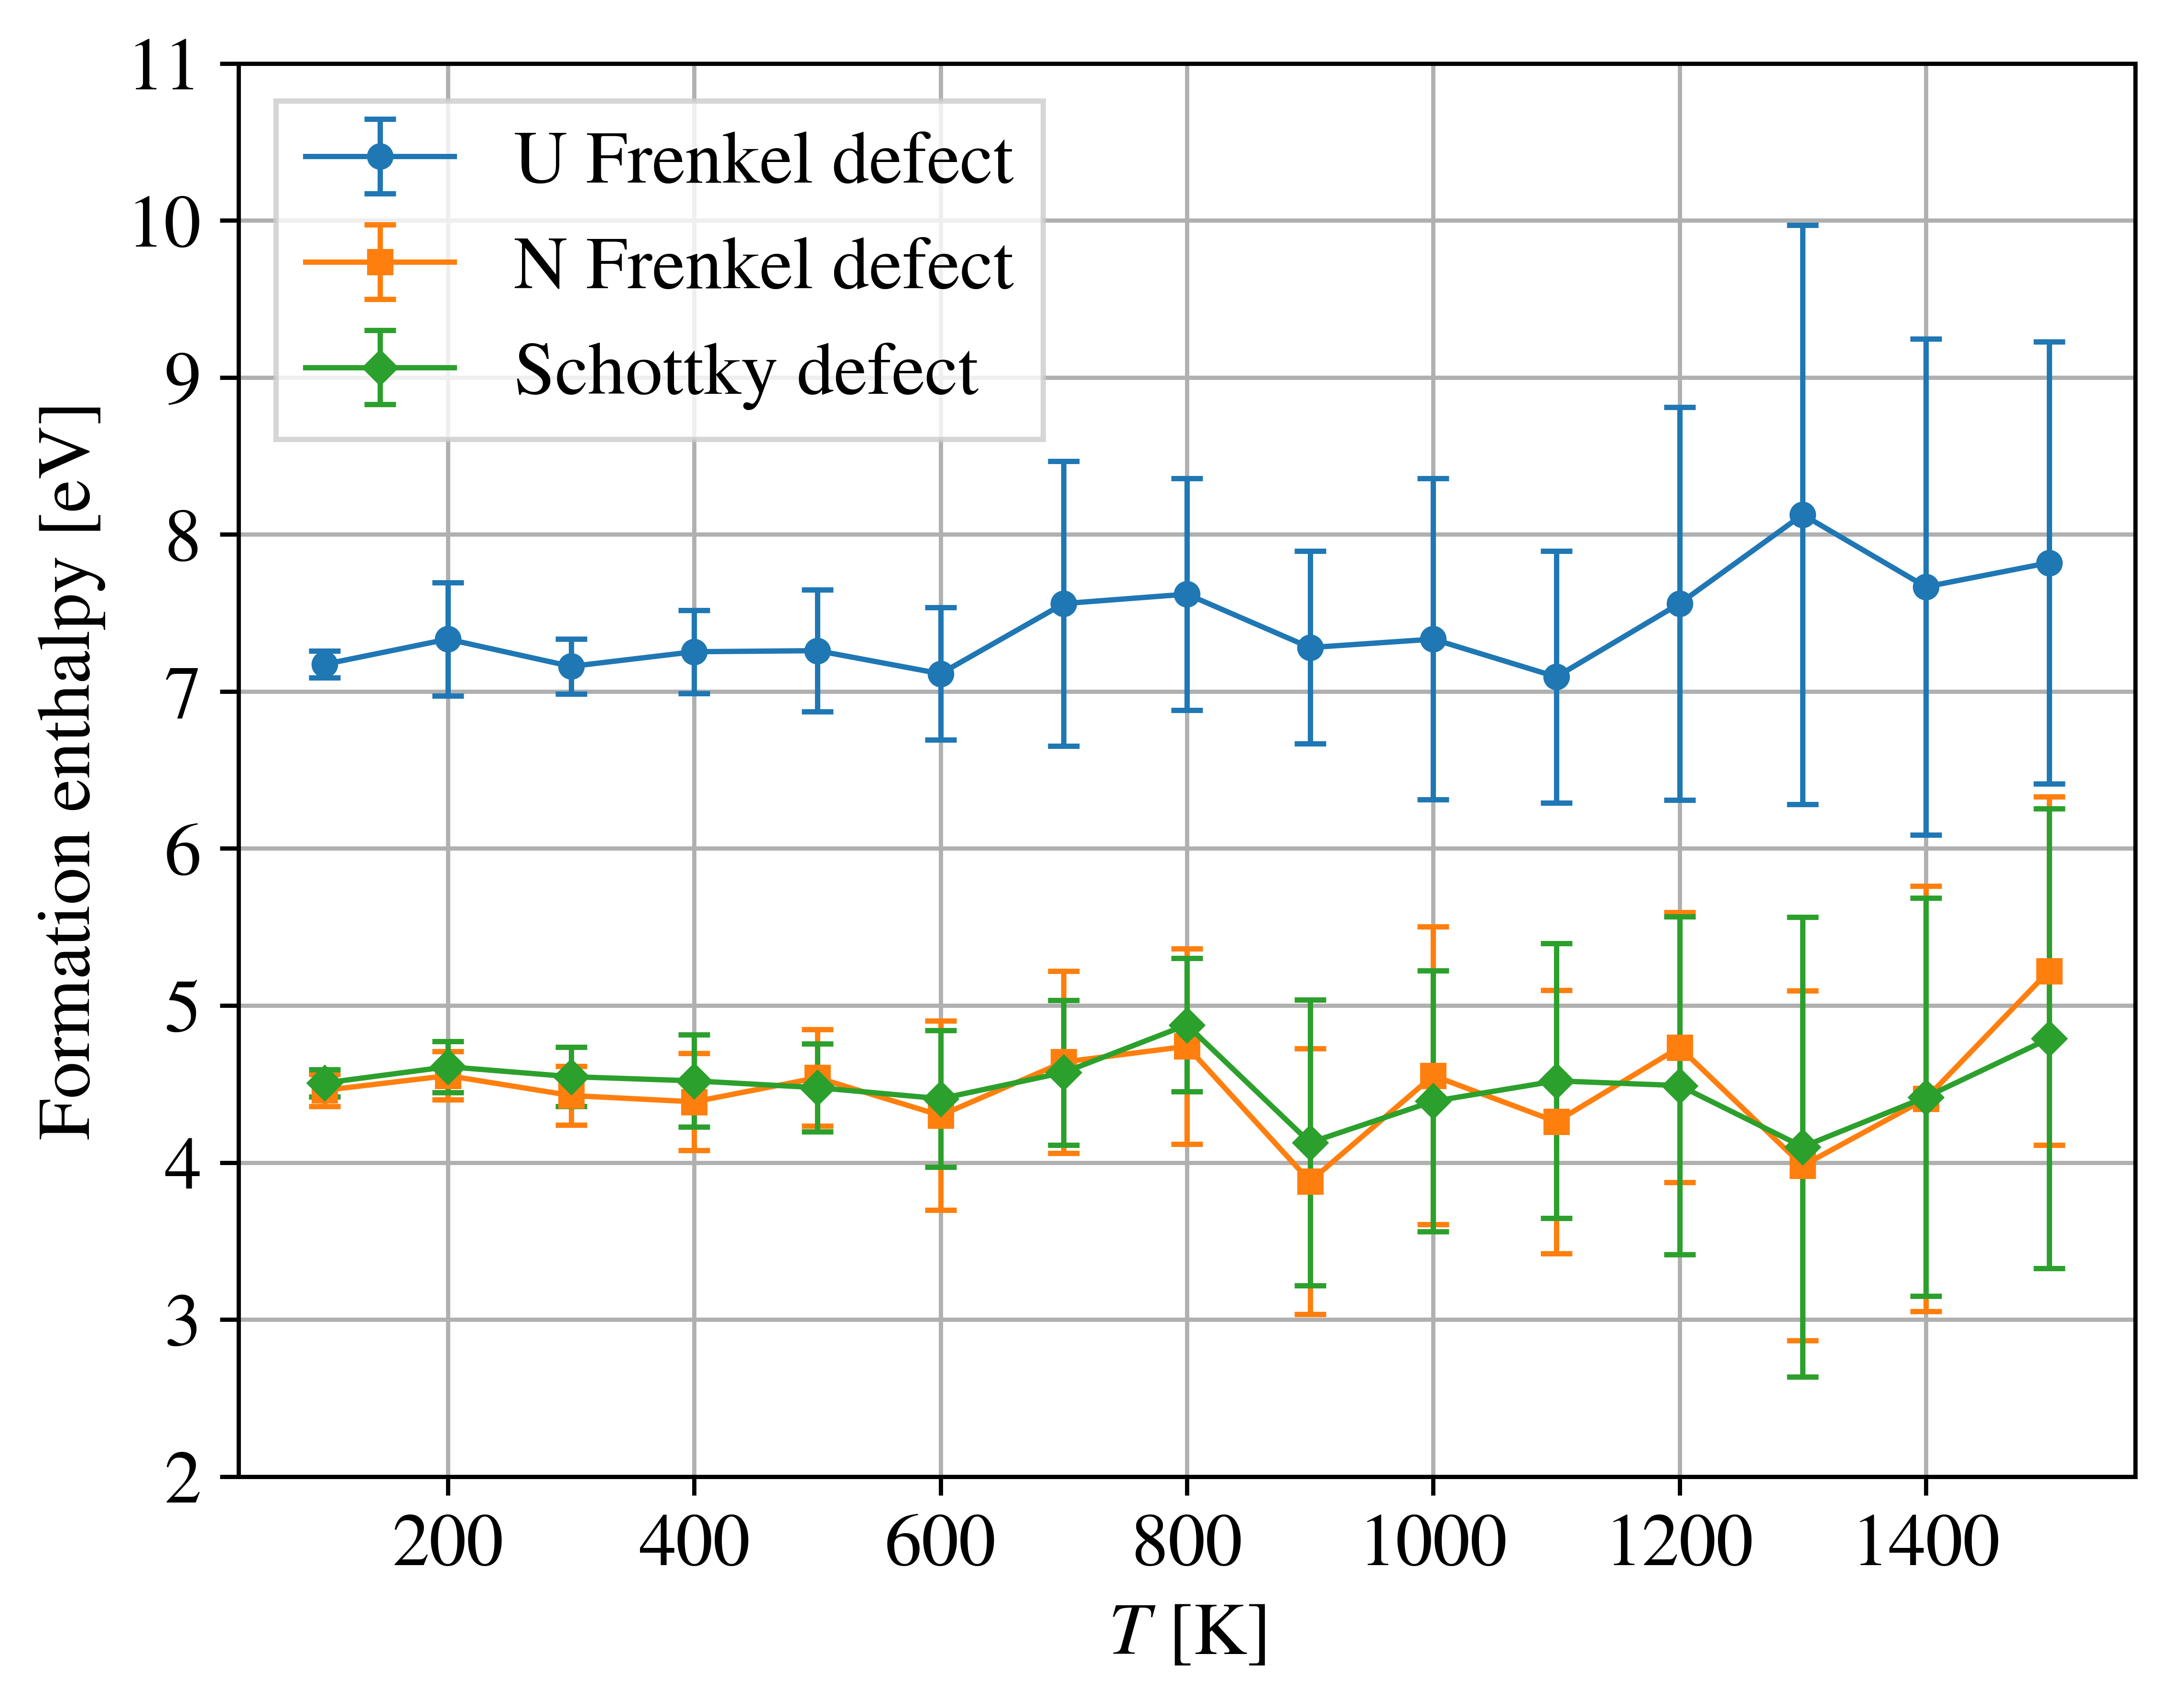
\includegraphics[width=0.50\textwidth]{FD-SD-T.png}
    \caption{Defect formation enthalpy as a function of temperature for the U Frenkel defect, N Frenkel defect, and Schottky defect in UN as a function of temperature as calculated by the Tseplyaev potential. Error bars correspond to one standard deviation.}
    \label{Fig:EfvsT}
\end{figure}

Formation enthalpies of U FD, N FD, and SD in UN as a function of temperature are shown in \cref{Fig:EfvsT}. As expected, the standard deviation increases with increasing temperature. The average formation enthalpy of U FD is confined to about 7-8 eV, whereas those of N FD and SD are confined to about 4-5 eV, with no apparent dependence on temperature.



\subsection{\ce{UN2}, $\alpha$-\ce{U2N3} and $\beta$-\ce{U2N3}}

\subsubsection{Thermophysical properties}

The \ce{UN2} lattice parameter and $C_P$ predicted by both potentials are shown in \cref{Fig:UN2a,Fig:UN2CP}, respectively. The Tseplyaev potential gives a better prediction of the \ce{UN2} lattice parameter with a slight underestimation and predicts a phase transition at about 800 K. On the other hand, the Kocevski potential overestimates the \ce{UN2} lattice parameter and predicts a stable \ce{UN2} structure up to 1400 K. It should be noted that the phase transition temperature of \ce{UN2} is 1324-1405 K \cite{Uno2020, Okamoto1997}. It is also worth mentioning that Silva \textit{et al.} \cite{Silva2009} reported lattice constants of \ce{UN2} and $\alpha$-\ce{U2N3} as a function of temperature; however, their samples were not of high purity but rather included the \ce{UN2}/$\alpha$-\ce{U2N3} solid solution, and, thus, are not ideal for comparison. The Tseplyaev potential overestimates the \ce{UN2} $C_P$ compared to that calculated by the Kocevski potential, a trend that was also observed for UN. Due to the lack of experimental measurements, we compare the predicted $C_P$ with the Dulong–Petit value which, for a compound, is defined as $3 n R$, $n$ being the number of atoms per formula unit ($n$ = 3 for \ce{UN2}, and $n$ = 5 for $\alpha$- and $\beta$-\ce{U2N3}), and $R$ being the gas constant \cite{White2015}. The Dulong–Petit value serves as a theoretical lower limit on $C_P$ data for solids well above room temperature and is useful to compare against in the absence of experimental measurements. The \ce{UN2} $C_P$ predicted by both potentials approach the Dulong–Petit value around room temperature and deviate from it at higher temperatures, which is the theoretically expected trend.

\begin{figure}[h!]
\centering
\begin{subfigure}{0.45\textwidth}
    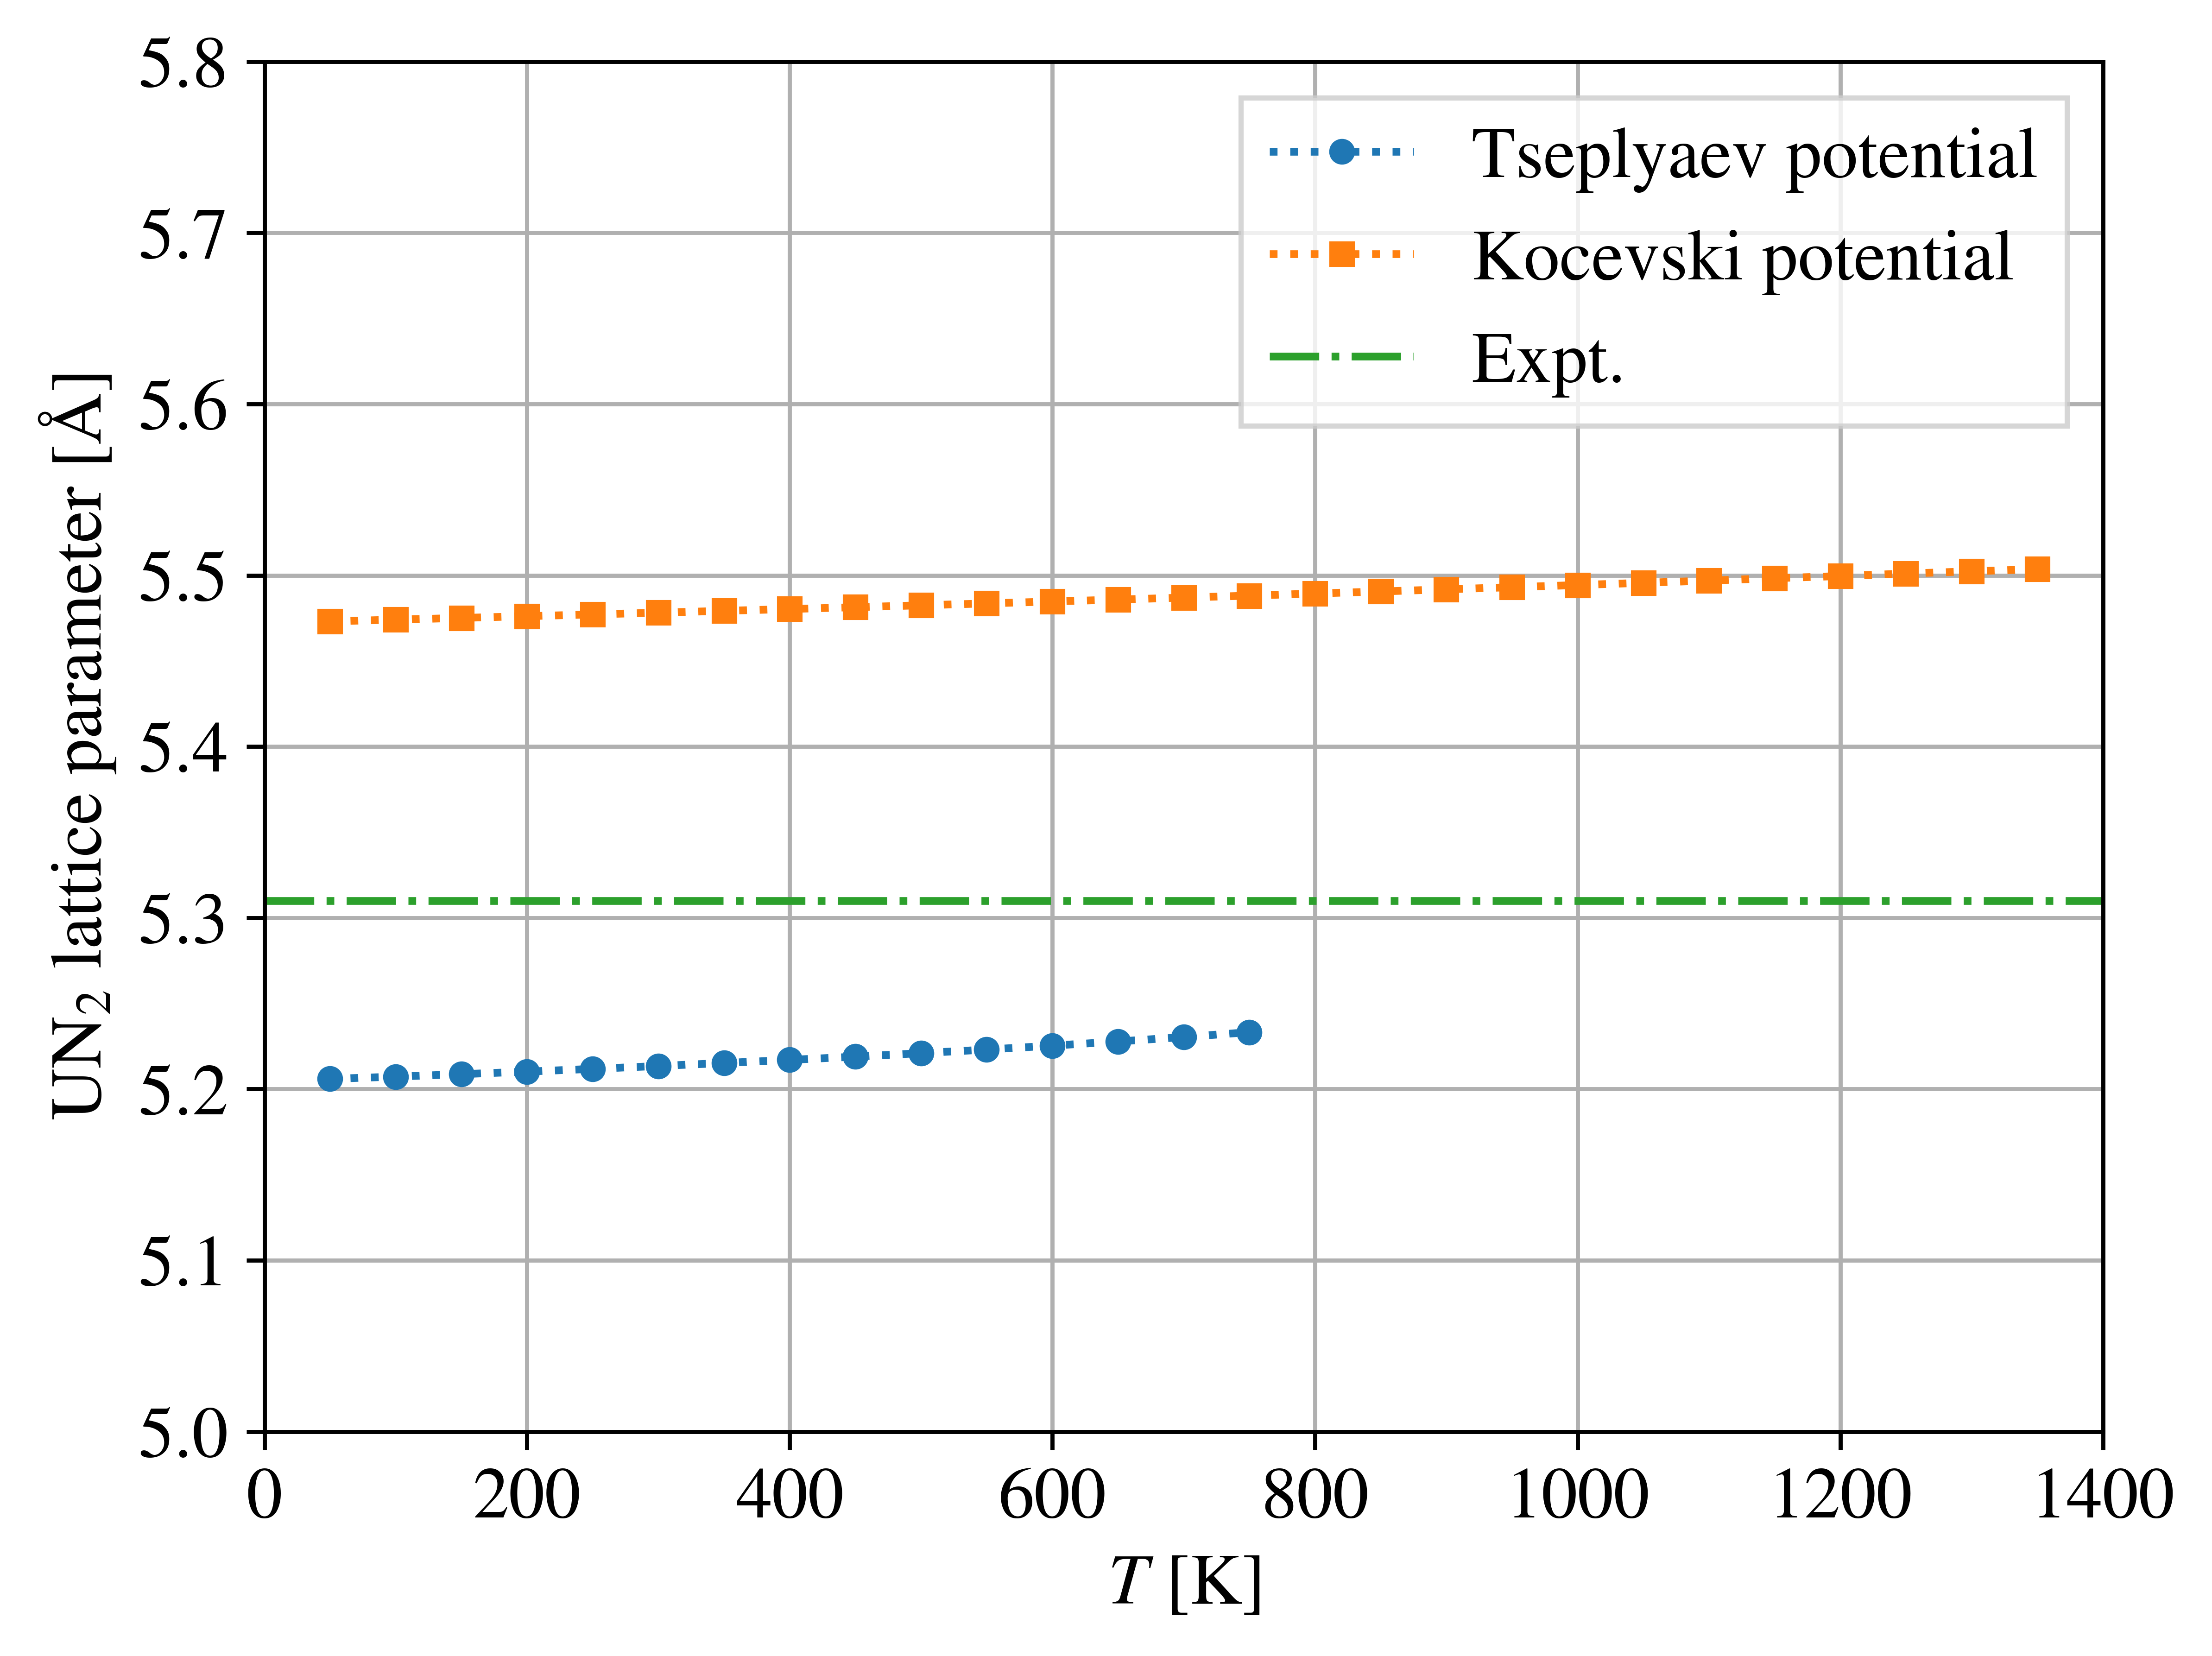
\includegraphics[width=\textwidth]{UN2a.png}
    \caption{}
    \label{Fig:UN2a}
\end{subfigure}
\hfill
\begin{subfigure}{0.45\textwidth}
    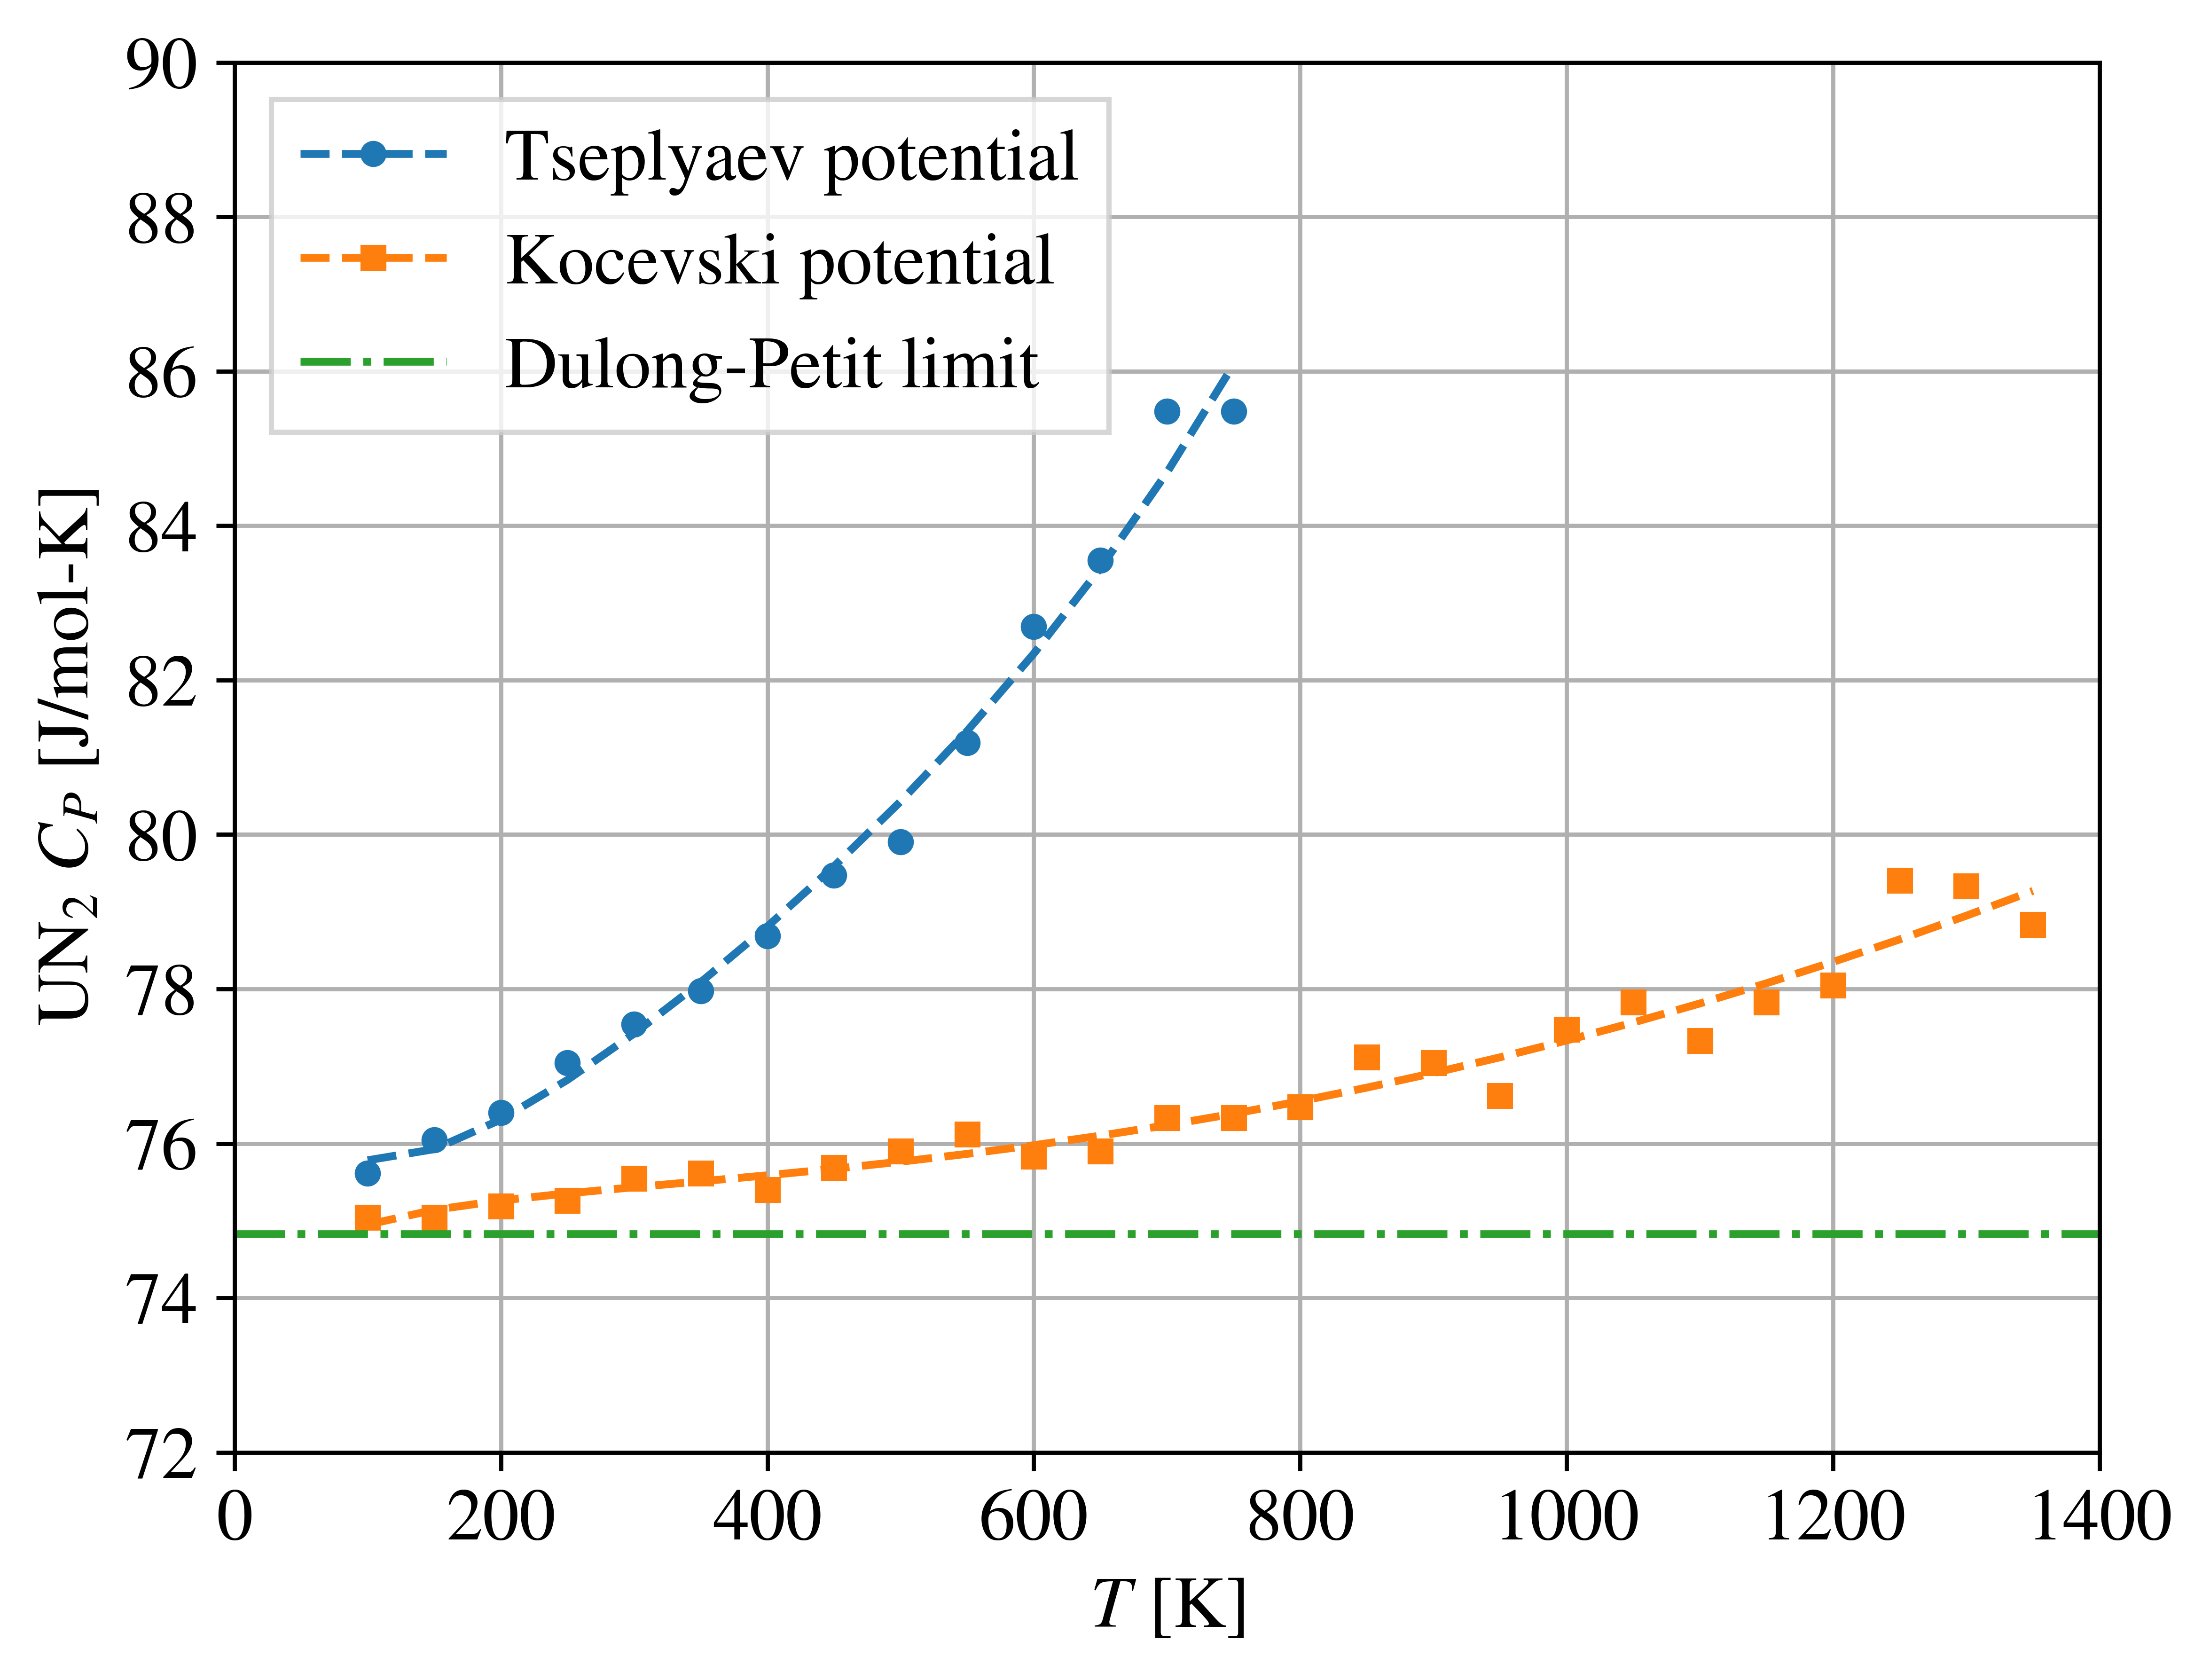
\includegraphics[width=\textwidth]{UN2CP.png}
    \caption{}
    \label{Fig:UN2CP}
\end{subfigure}
\caption{\textbf{(a)} The lattice parameter of \ce{UN2} calculated by both potentials as a function of temperature. \textbf{(b)} \ce{UN2} $C_P$ calculated by both potentials as a function of temperature. $C_P$ calculated by the Tseplyaev and Kocevski potentials are fitted to \cref{CPUN2ADP,CPUN2EAM}, respectively. The experimental lattice parameter of \ce{UN2} is taken from Lu \textit{et al.} \cite{Lu2011} and included as a horizontal line because the temperature at which it was measured is not reported.}
\label{Fig:UN2}
\end{figure}

The Tseplyaev potential could not predict a stable structure above 0 K for either $\alpha$-\ce{U2N3} or $\beta$-\ce{U2N3}, so we only discuss the finite temperature $\alpha$- and $\beta$-\ce{U2N3} properties predicted by the Kocevski potential (\cref{Fig:U2N3}). The Kocevski potential predicts that the $\alpha$-\ce{U2N3} phase is mechanically stable up to about 1000 K. For $\alpha$-\ce{U2N3}, the Kocevski potential overestimates the lattice parameter, and for $\beta$-\ce{U2N3}, it overestimates the $a$ parameter and underestimates the $c$ parameter. The $\alpha$- and $\beta$-\ce{U2N3} $C_P$ predicted by the Kocevski potential nearly coincide and approach the Dulong–Petit value around RT. Additionally, the Kocevski potential predicts that the $\beta$-\ce{U2N3} structure can be mechanically stable at very low temperatures.

As mentioned earlier, the Tseplyaev potential is a modified version of the ADP developed by Kuskin \textit{et al.} \cite{Kuksin2016}. The authors reported that Kuksin's potential could stabilize the structures of $\alpha$- and $\beta$-\ce{U2N3}. However, Tseplyaev and Starikov \cite{Tseplyaev2016} don't report any capability of the modified version of the potential to simulate polymorphs of \ce{U2N3} at zero pressure. Thus, it appears that in the modification of the potential to improve UN property prediction, the capability was lost for other phases in the U-N system.



\subsubsection{Elastic properties}

The 0 K elastic constants of \ce{UN2} are shown in \cref{Tab:ECUN2}. The predictions of the Kocevski potential show a good agreement with the DFT predictions for $C_{12}$ and $C_{44}$, whereas it underestimates $C_{11}$ by about 40\%. The predictions of the Tseplyaev potential show much larger errors: it overestimates $C_{11}$ and $C_{12}$ by more than 70\%, and 40\%, respectively, and its $C_{44}$ value is overestimated by nearly a factor of 5. The temperature dependence of the \ce{UN2} elastic constants and moduli are shown in \cref{Fig:ECUN2}. The Kocevski potential shows general qualitative agreement with the \ce{UN2} elastic moduli predicted by DFT, whereas the Tseplyaev potential greatly overestimates all elastic moduli and fails to give qualitative predictions. The Kocevski potential shows minimal softening of the \ce{UN2} elastic properties with increasing temperature.

\begin{table}[h!]
    \centering
    \caption{\ce{UN2} elastic constants (GPa) at 0 K as calculated by both potentials. The DFT values are from Lu \textit{et al.} \cite{Lu2011} and have been calculated using the GGA+$U$ approach with $U$ = 2 eV.}
    \footnotesize
    \begin{tabular}{c|ccc}
    \hline
                             & $C_{11}$ & $C_{12}$ & $C_{44}$ \\
    \hline          
    Tseplyaev potential    & 856.2    & 201.4    & 291.7    \\
    Kocevski potential     & 275.9    & 184.1    & 67.8     \\
    DFT \cite{Lu2011}        & 488.2    & 140.5    & 55.3     \\
    \hline
    \end{tabular}
    \label{Tab:ECUN2}
\end{table}

\begin{figure}[h!]
\centering
\begin{subfigure}{0.45\textwidth}
    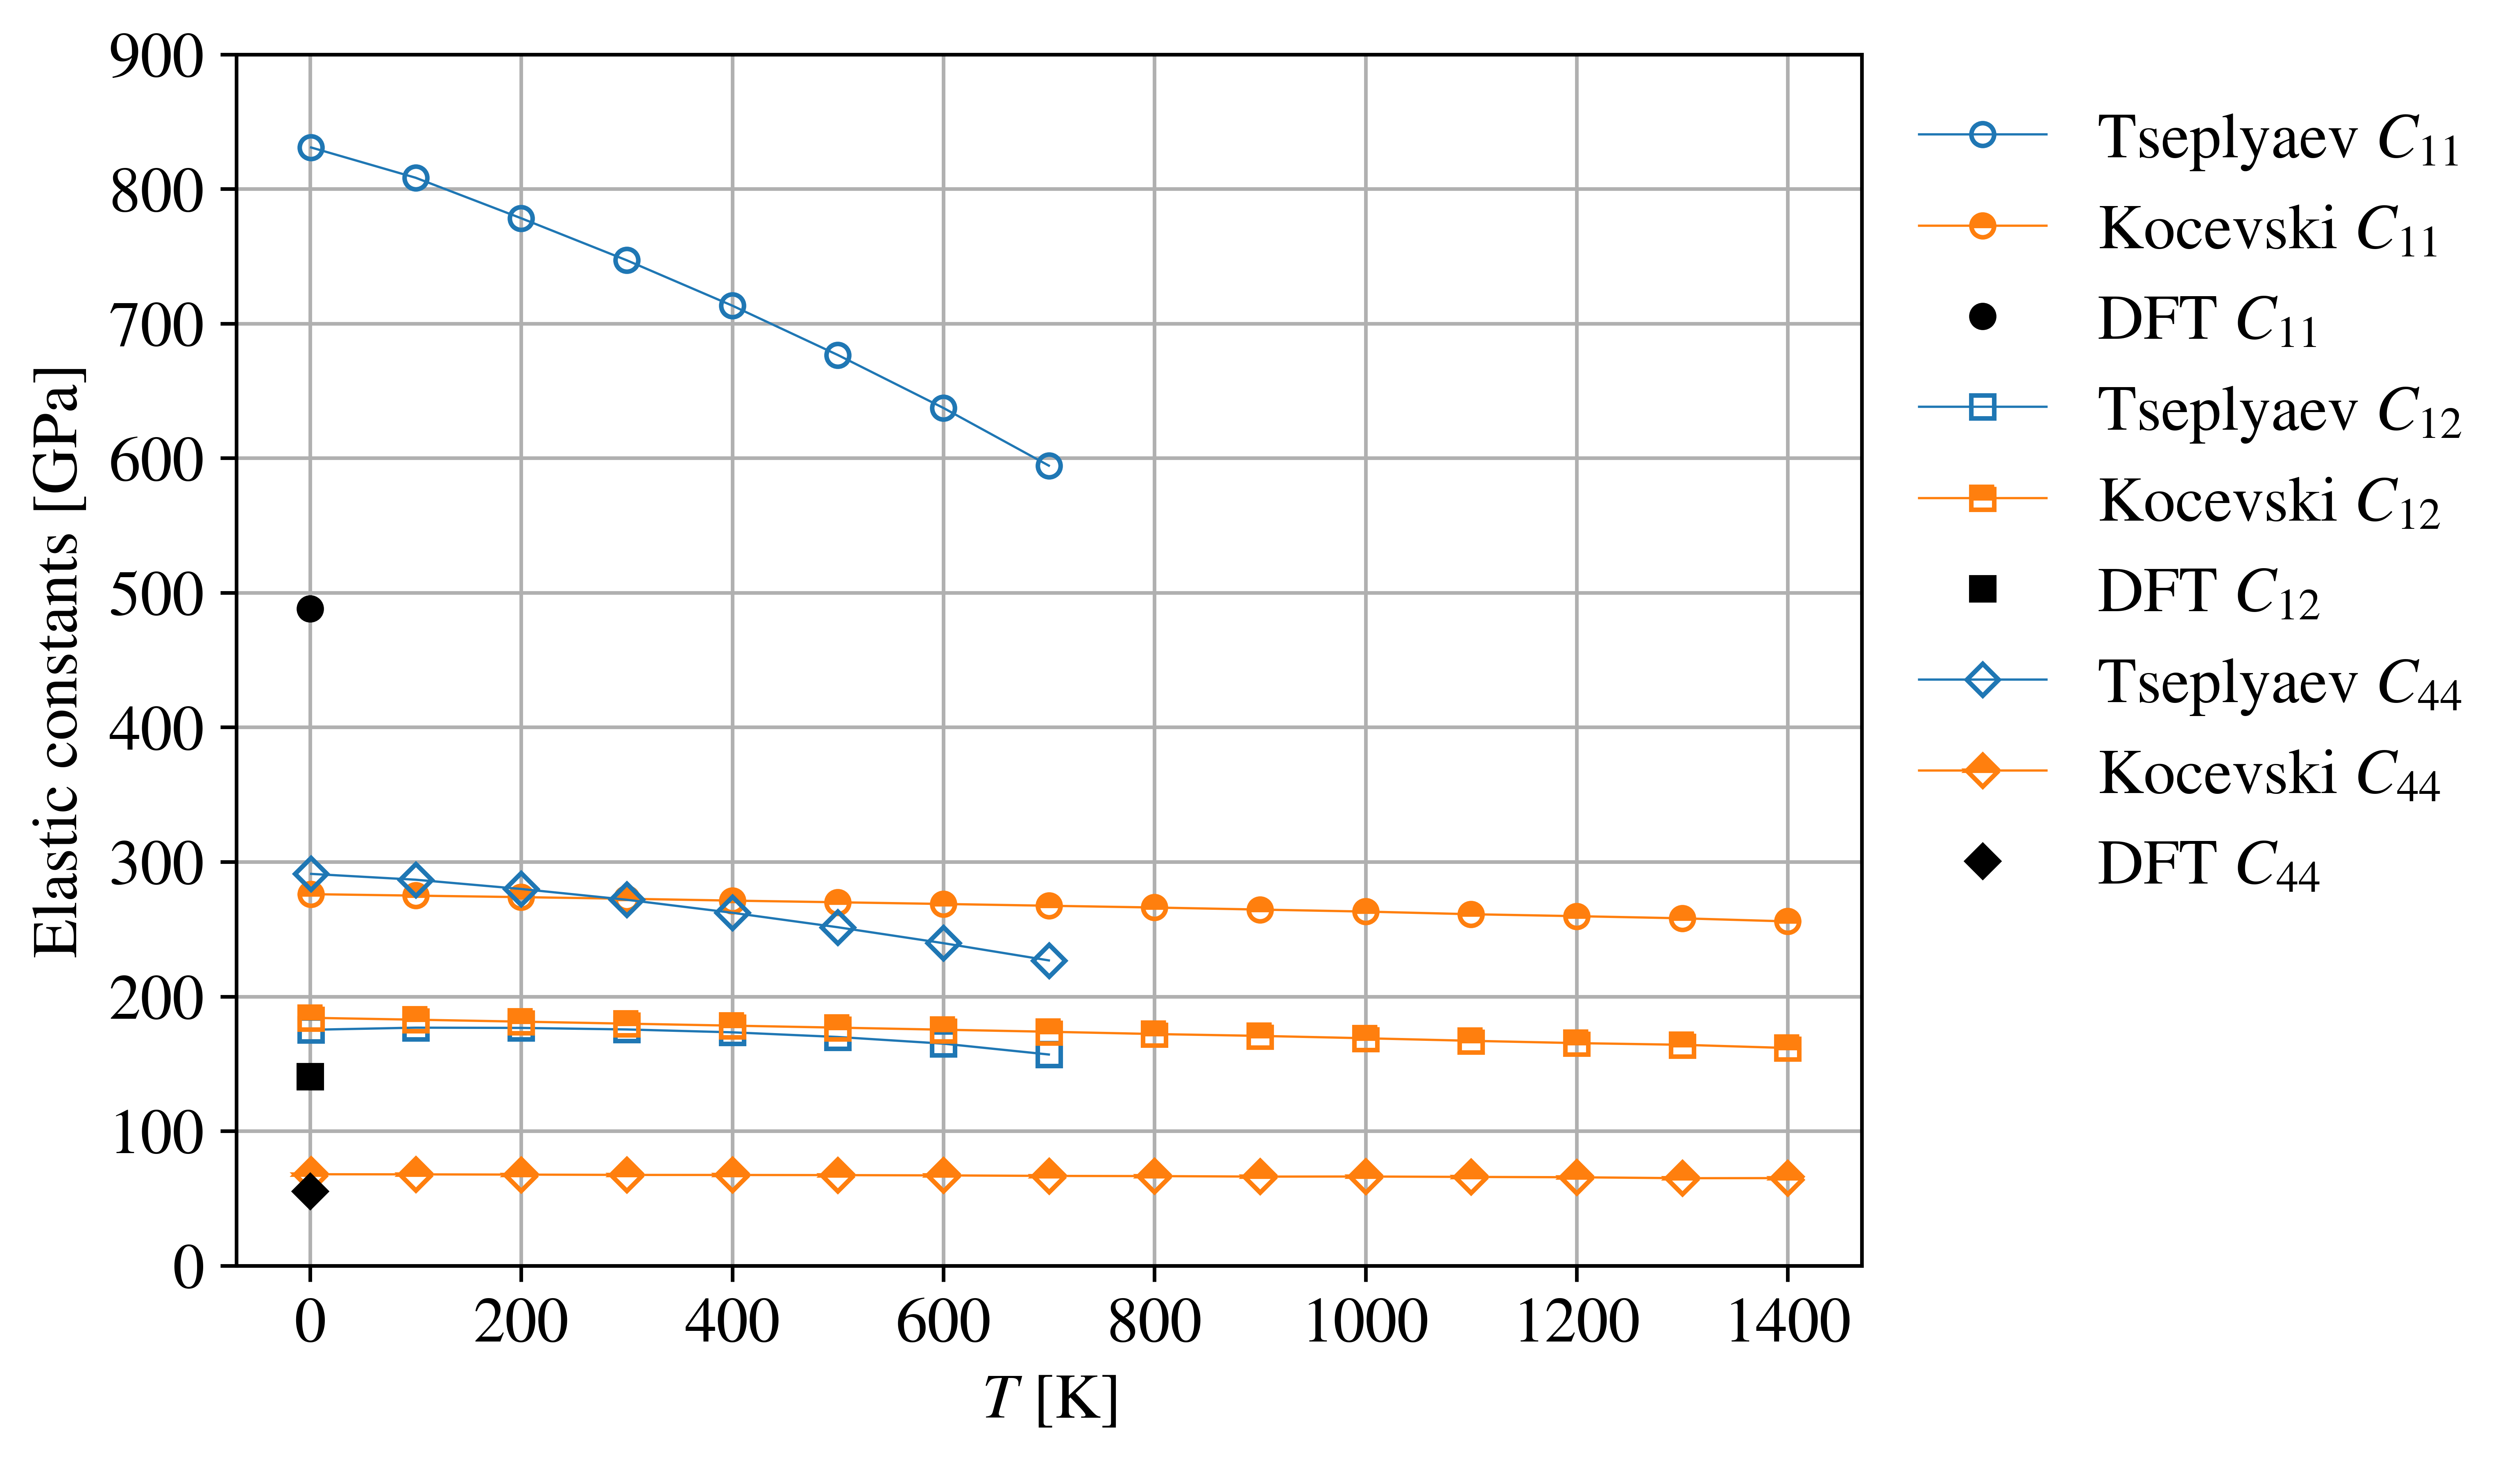
\includegraphics[width=\textwidth]{ElasticConstantsUN2.png}
    \caption{}
    \label{Fig:ElasConstUN2}
\end{subfigure}
\hfill
\begin{subfigure}{0.45\textwidth}
    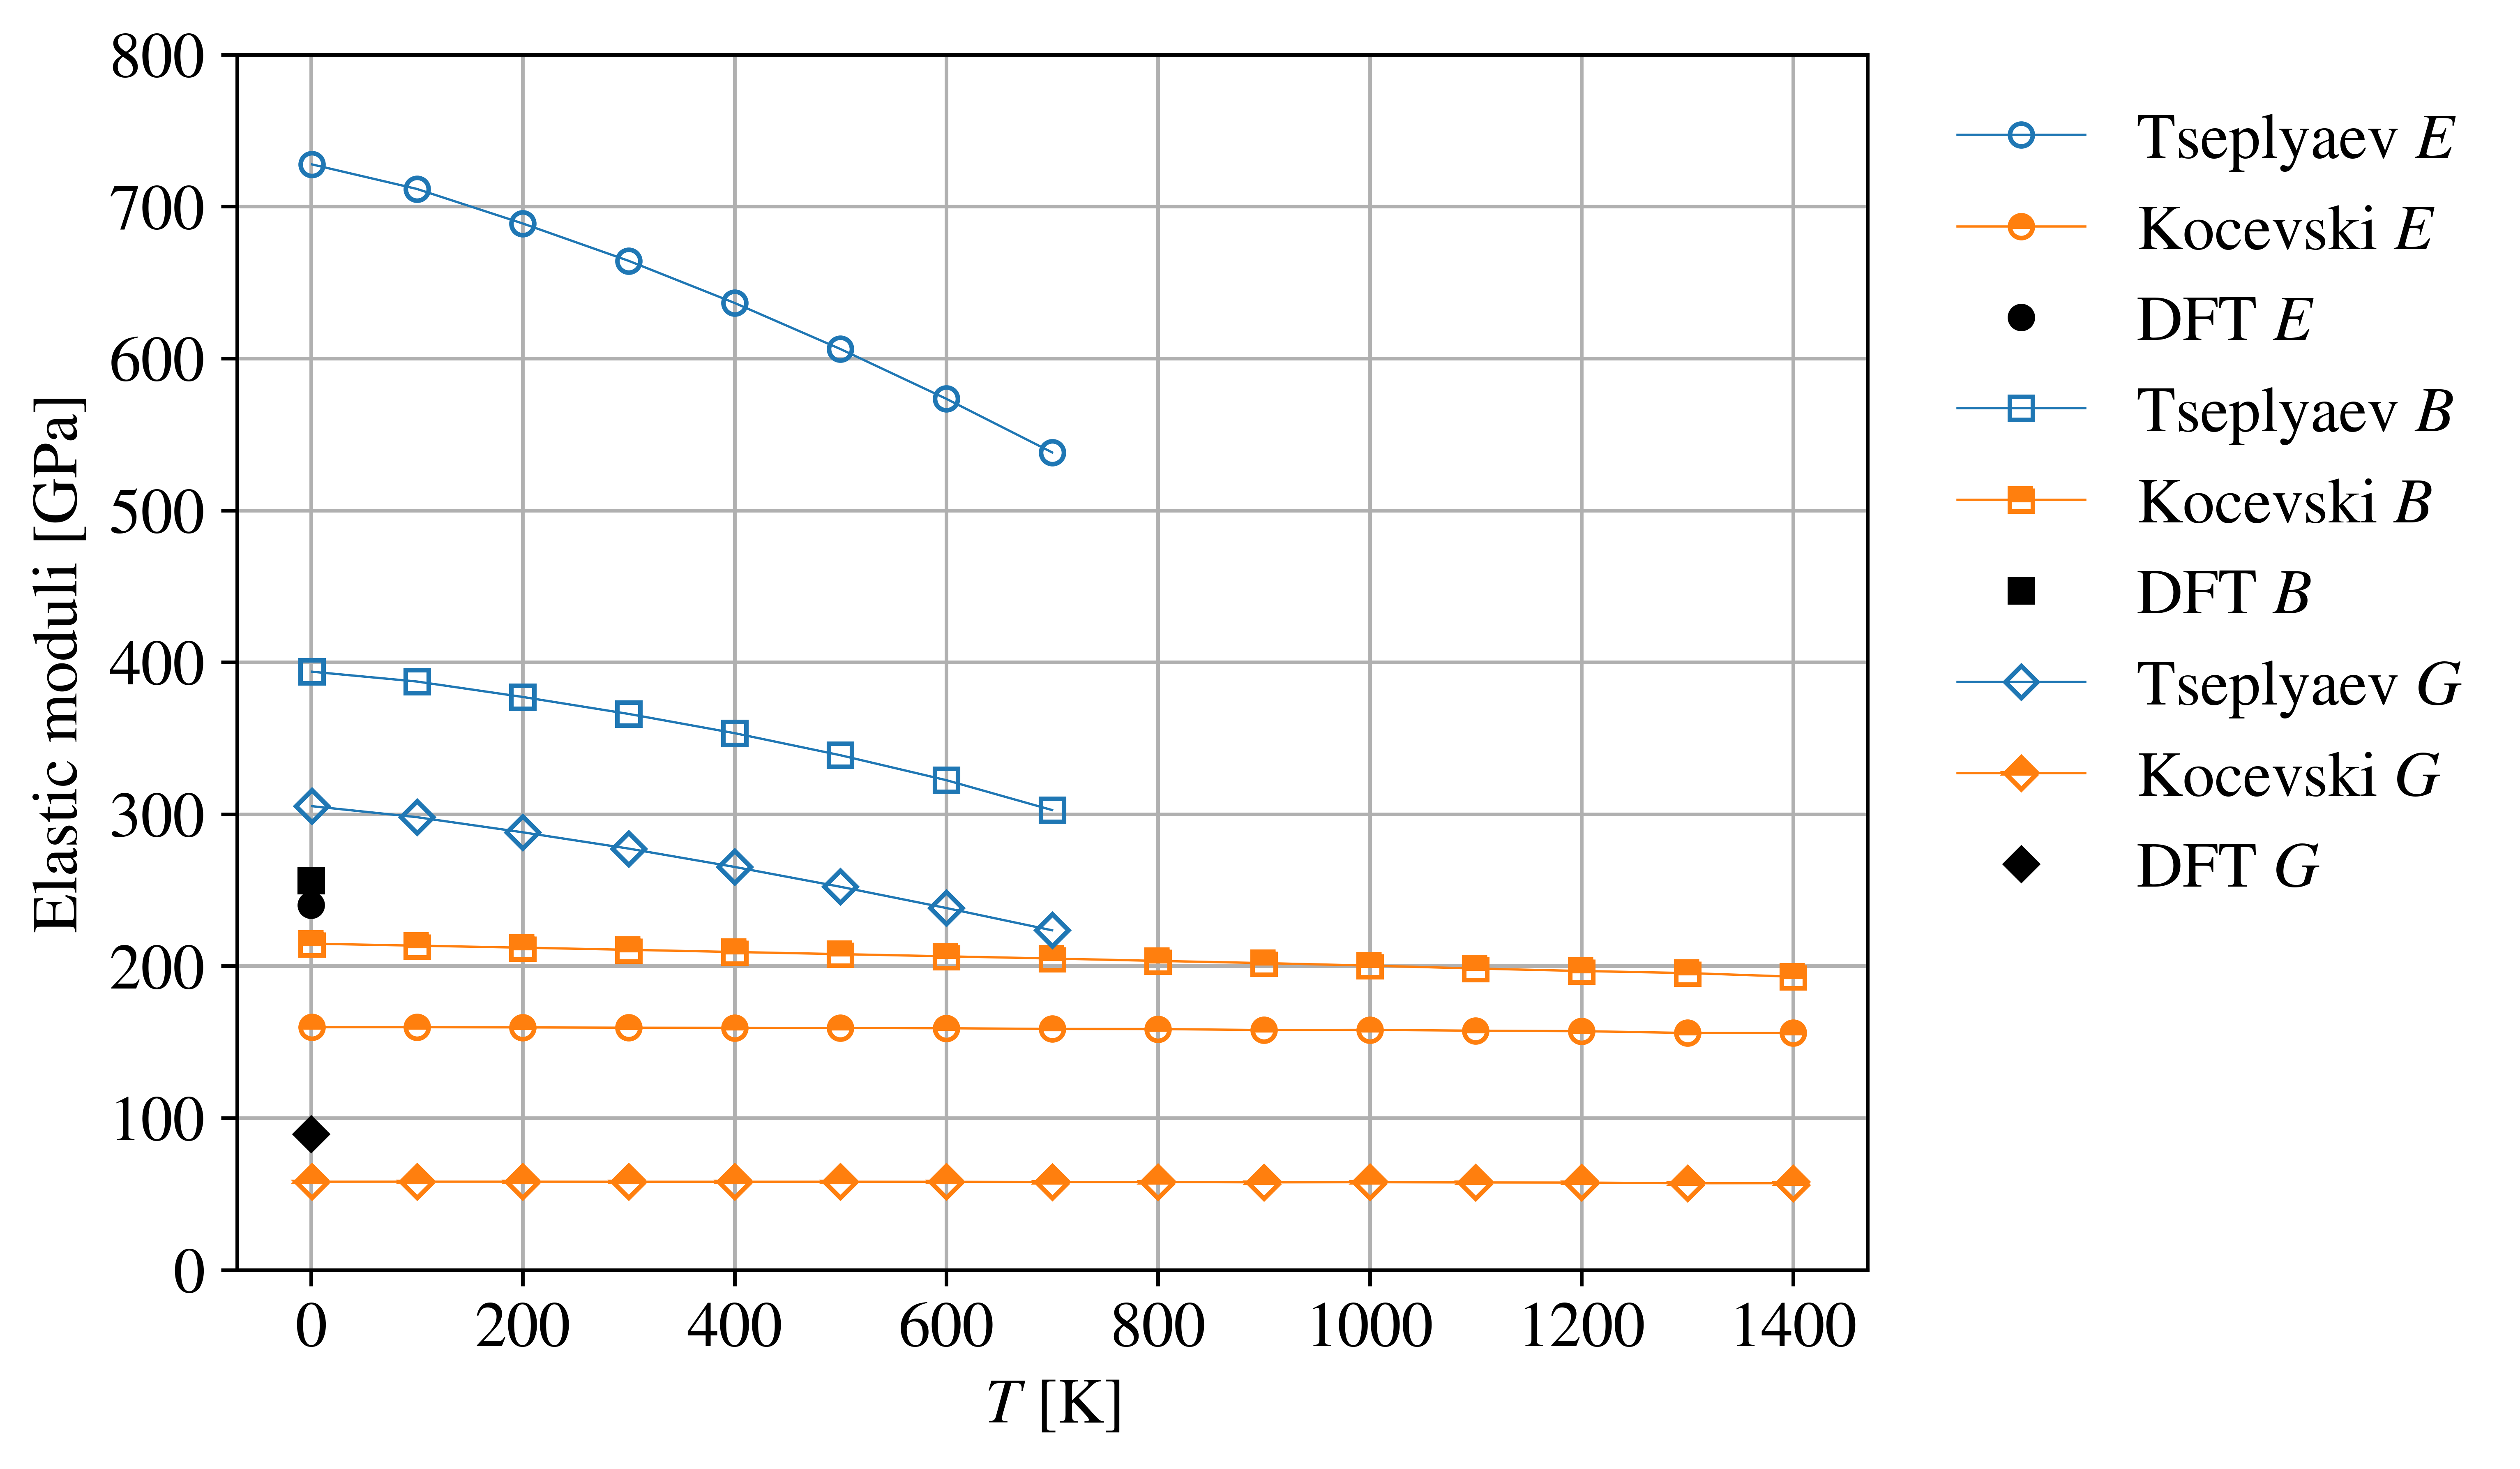
\includegraphics[width=\textwidth]{ElasticModuliUN2.png}
    \caption{}
    \label{Fig:ElasModUN2}
\end{subfigure}
\hfill
% \begin{subfigure}{0.45\textwidth}
%    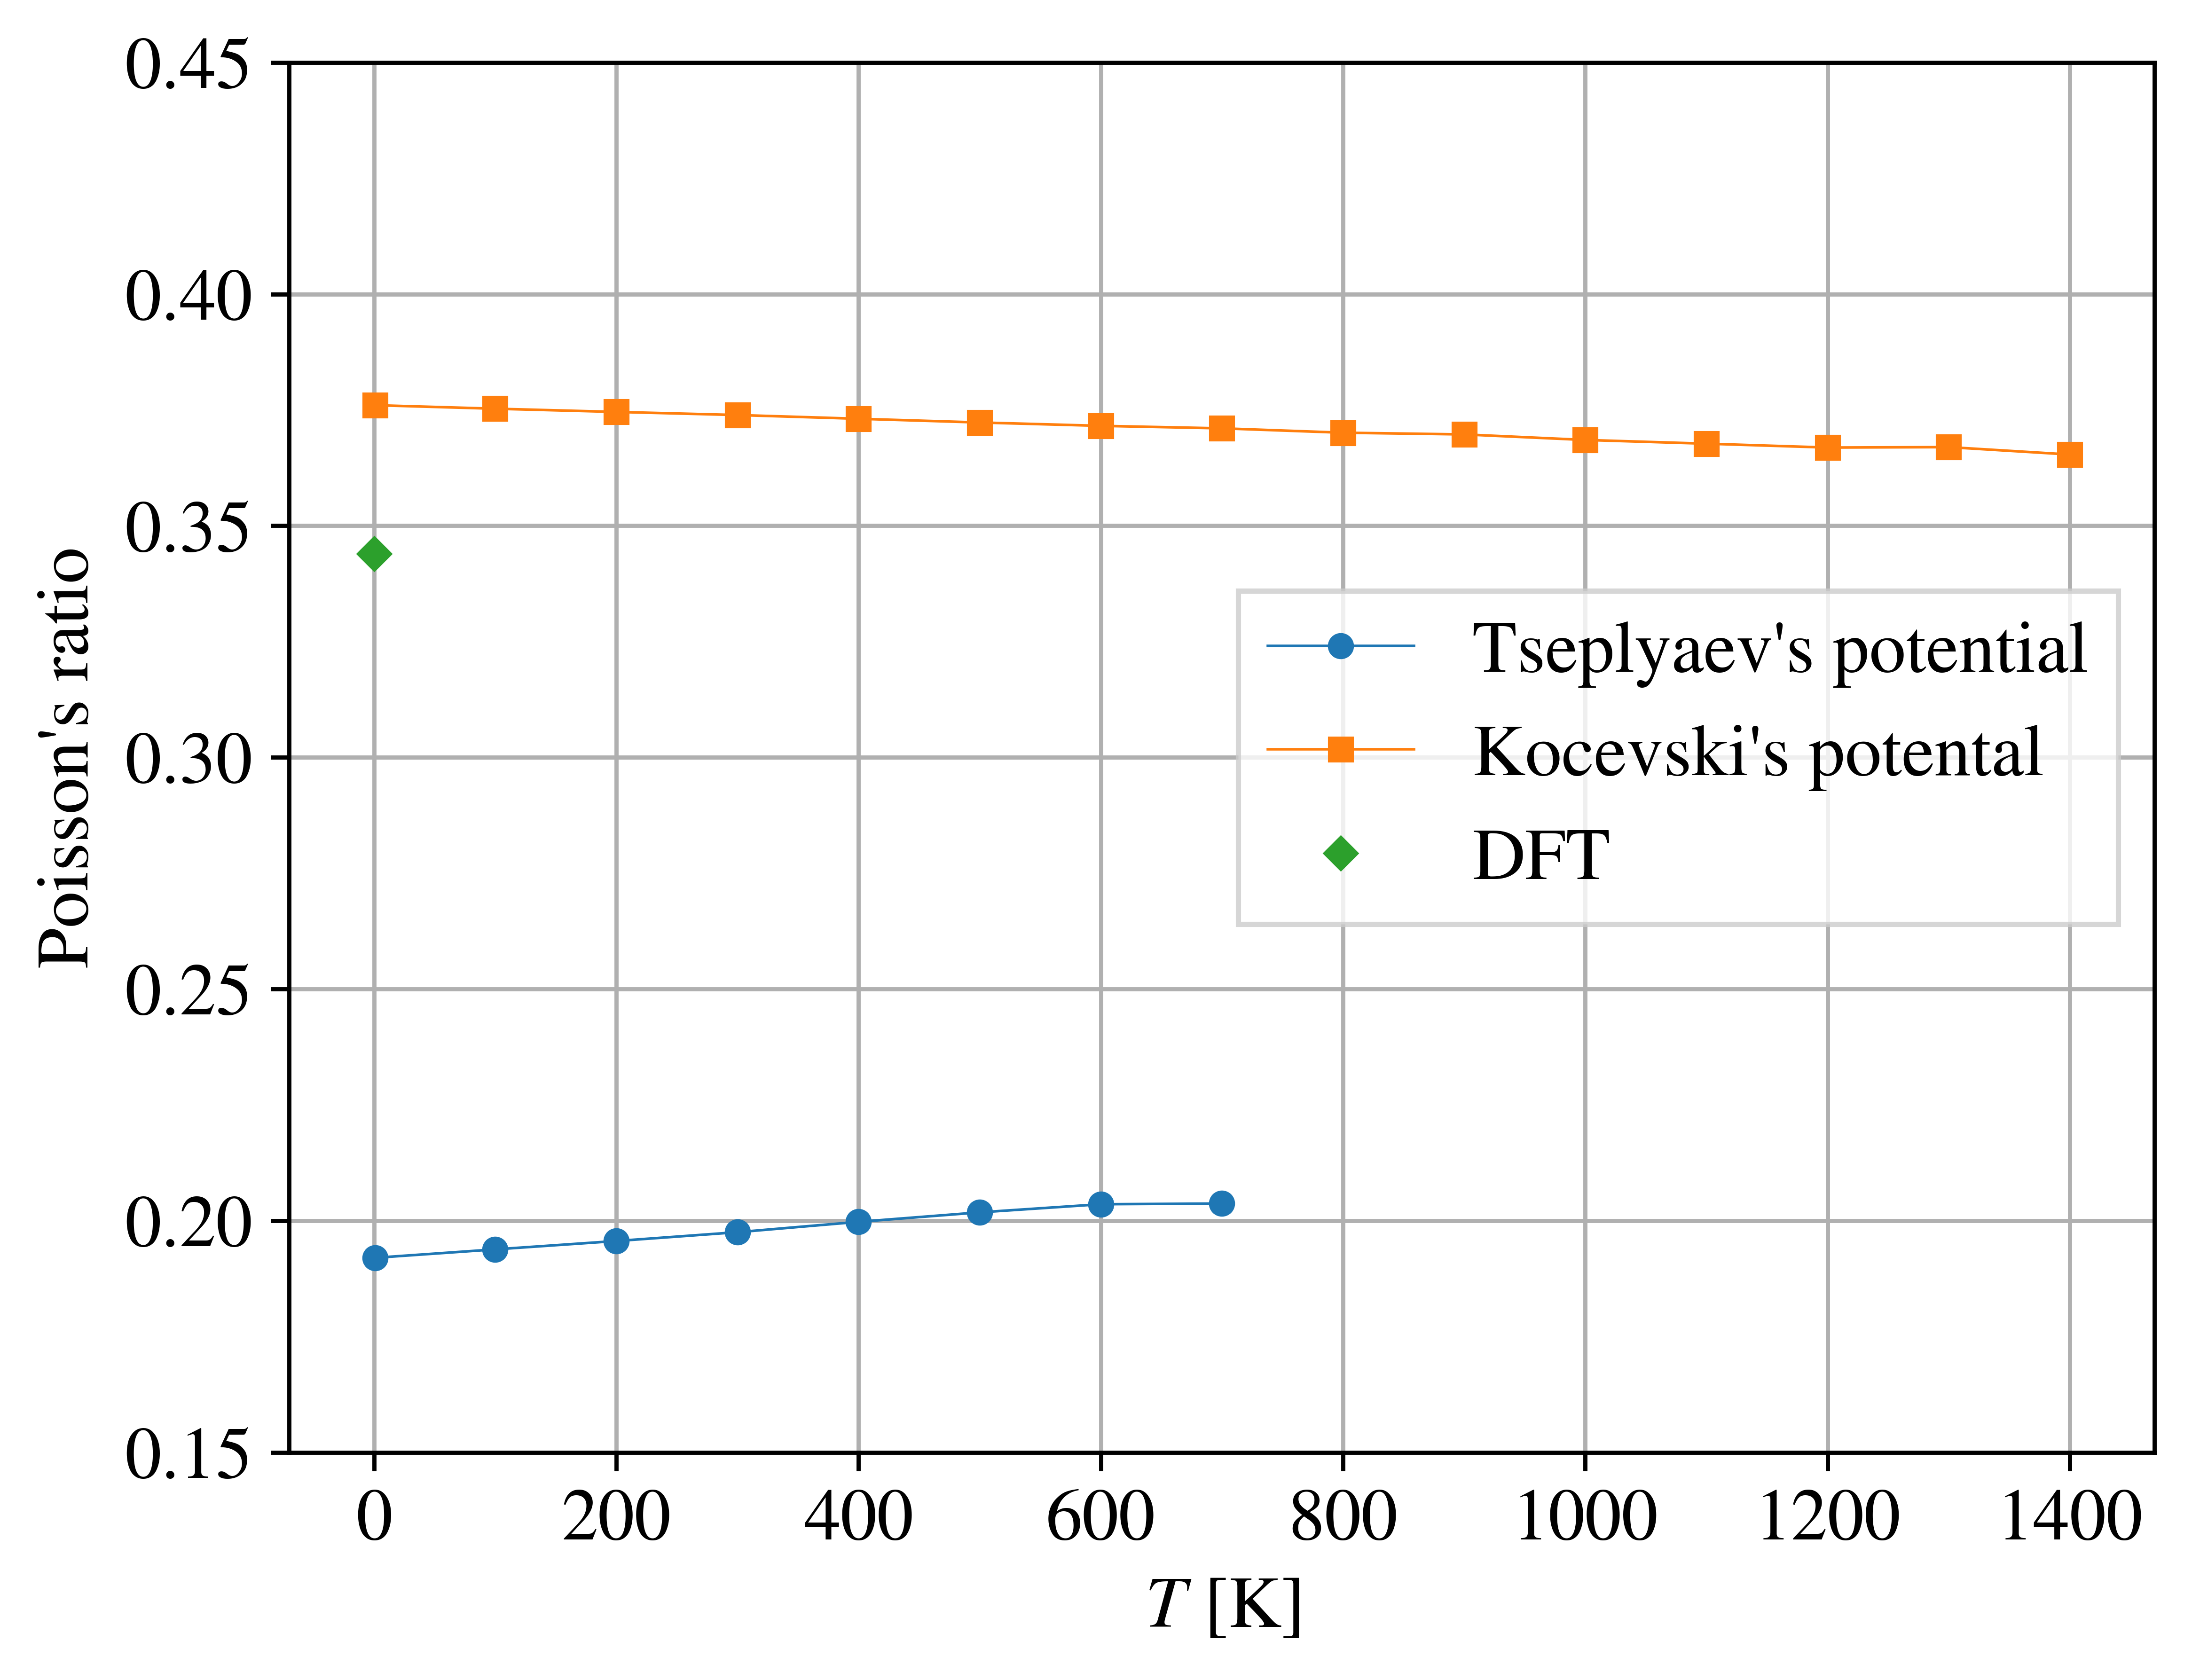
\includegraphics[width=\textwidth]{PoissonRatioUN2.png}
%    \caption{}
%   \label{Fig:PoissonUN2}
% \end{subfigure}
\caption{The predicted temperature variation of \textbf{(a)} \ce{UN2} elastic constants, $C_{11}$, $C_{12}$, and $C_{44}$, \textbf{(b)} \ce{UN2} Young's modulus, $E$, bulk modulus, $B$, and shear modulus, $G$. The DFT values are from Lu \textit{et al.} \cite{Lu2011}.}
% and \textbf{(c)} Poisson's ratio. 
\label{Fig:ECUN2}
\end{figure}

The 0 K elastic constants of $\alpha$-\ce{U2N3} calculated by the Kocevski potential are $C_{11}$ = 185.4 GPa, $C_{22}$ = 141.8 GPa, and $C_{44}$ = 41.8 GPa, whereas the elastic constants and moduli calculated at finite temperatures are shown in \cref{Fig:ElasConstaU2N3,Fig:ElasModaU2N3}, respectively. To the best of our knowledge, no experimental or DFT elastic property data exist for $\alpha$-\ce{U2N3}. It can be observed that $\alpha$-\ce{U2N3} is generally softer than \ce{UN2} which is expected because, as explained earlier, the $\alpha$-\ce{U2N3} conventional unit cell lacks 16 N atoms, and thus has fewer bonds compared to the $2 \times 2 \times 2$ \ce{UN2} supercell.

For $\beta$-\ce{U2N3}, the 0 K elastic constants are shown in \cref{Tab:ECU2N3}. The predictions of both potentials satisfy the stability criteria of the hexagonal lattice and nearly agree, except for $C_{33}$ which the Tseplyaev potential overpredicts by a factor of 23, and $C_{44}$ which the Tseplyaev potential underestimates with an error of about 50\%--all relative to the values predicted by the Kocevski potential at 0 K. The bulk modulus predicted by the Kocevski potential agrees perfectly with that predicted by the DFT study of Lu \textit{et al.} \cite{Lu2011}. The elastic constants and bulk modulus of $\beta$-\ce{U2N3} predicted by the Tseplyaev potential vary significantly by varying the strain, whereas those predicted by the Kocevski potential show a negligible dependence on the strain value. This is indicative of potential instabilities using the Tseplyaev potential for $\beta$-\ce{U2N3}, which are confirmed through the evaluation of the structure at finite temperatures, which decomposes as discussed. The variation of the $\beta$-\ce{U2N3} elastic constants with temperature is shown in \cref{Fig:ElasConstU2N3}. $C_{11}$ and $C_{33}$ show observable softening, $C_{12}$ shows a slower softening rate, and $C_{13}$ and $C_{44}$ are nearly constant. $\beta$-\ce{U2N3} elastic moduli are shown in \cref{Fig:ElasModU2N3}. As explained earlier, the predicted bulk modulus qualitatively agrees with DFT values. In general, further experimental investigations are required to validate the predicted properties of \ce{UN2}, $\alpha$-\ce{U2N3}, and $\beta$-\ce{U2N3}.

\begin{table}[h!]
    \centering
    \caption{$\beta$-\ce{U2N3} elastic properties (GPa) as calculated by both potentials. $B$ = 232 GPa has been calculated by Evarestov \textit{et al.} \cite{Evarestov2008} using the LCAO DFT approach. $B$ = 209.2 GPa has been calculated by Lu \textit{et al.} \cite{Lu2011} using the GGA+$U$ approach with $U$ = 2 eV.}
    \footnotesize
    \begin{tabular}{c|ccccc|c}
    \hline
                  & $C_{11}$ & $C_{12}$ & $C_{13}$ & $C_{33}$ & $C_{44}$ & $B$ \\
    \hline
    Tseplyaev potential           & 372.4    & 166.8    & 118.1    & 5680.1   & 30.0     & 534.5 \\
    
    Kocevski potential & 357.0    & 224.2    & 140.7    & 242.7    & 64.5     & 210.0 \\
    
    DFT           &          &          &          &          &          & 232 \cite{Evarestov2008}, 209.2 \cite{Lu2011} \\
    \hline
    \end{tabular}
    \label{Tab:ECU2N3}
\end{table}

\begin{figure}[h!]
\centering
\begin{subfigure}{0.45\textwidth}
    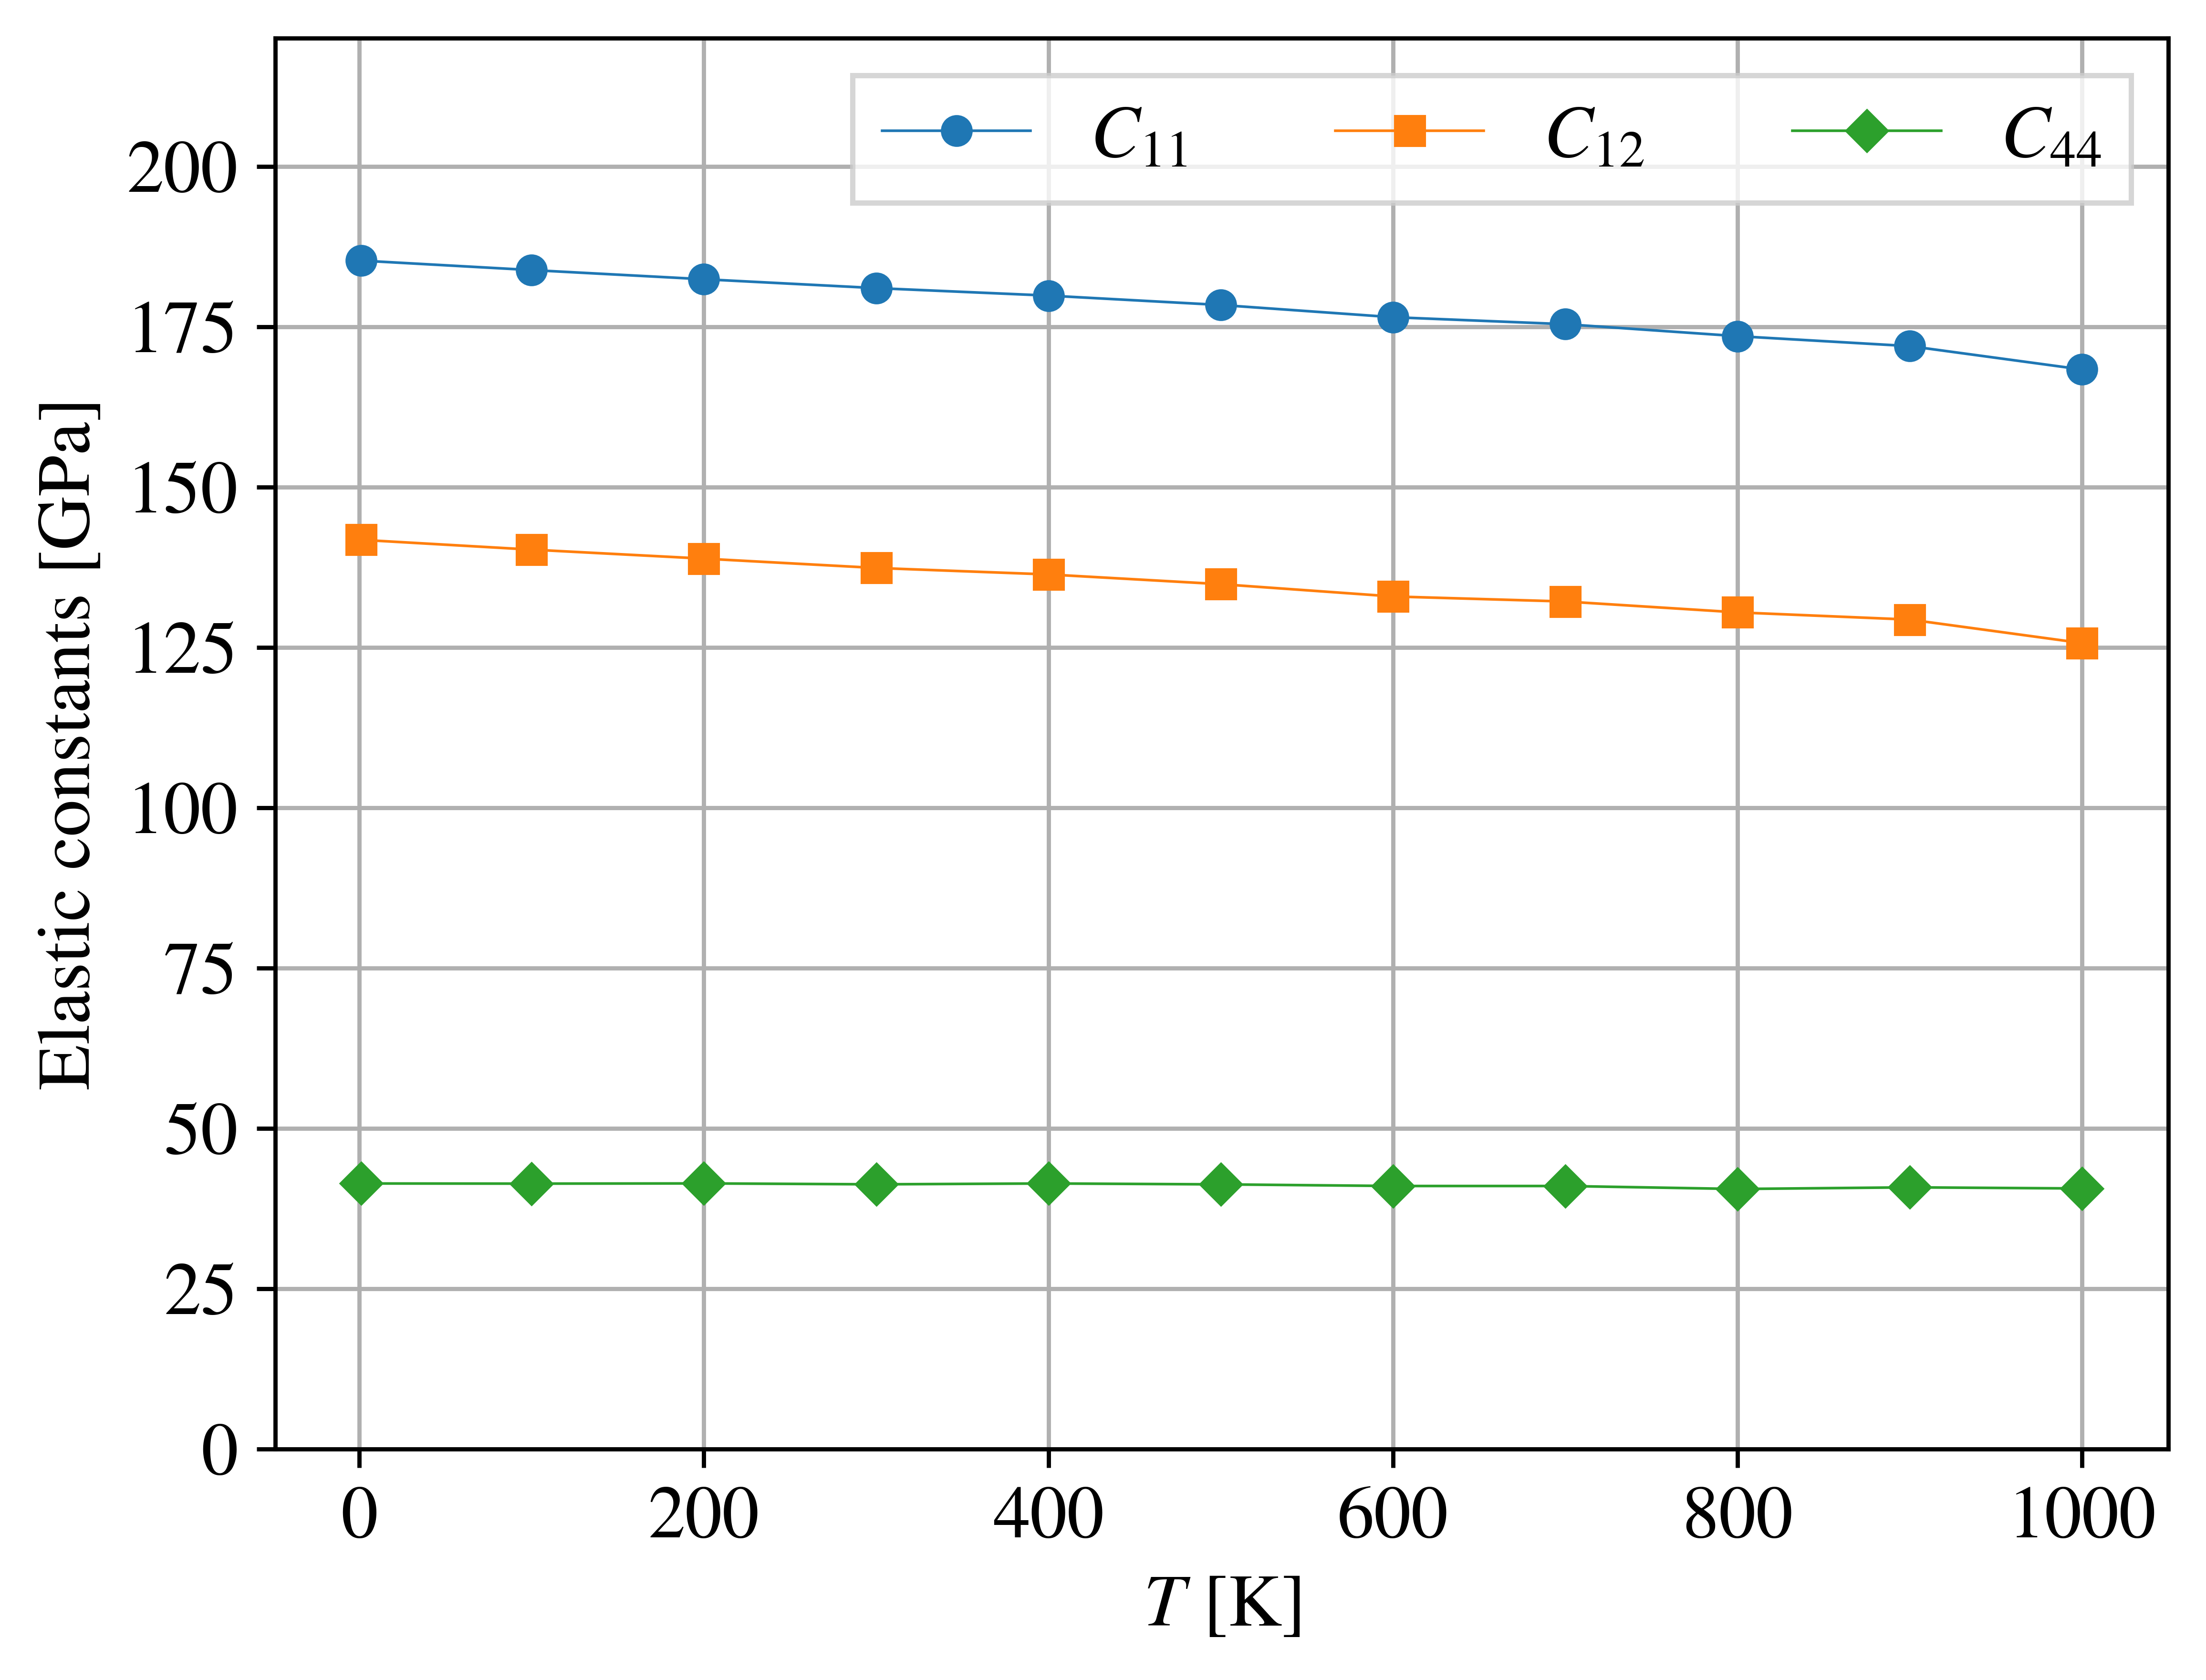
\includegraphics[width=\textwidth]{ElasticConstantsaU2N3.png}
    \caption{}
    \label{Fig:ElasConstaU2N3}
\end{subfigure}
\hfill
\begin{subfigure}{0.45\textwidth}
    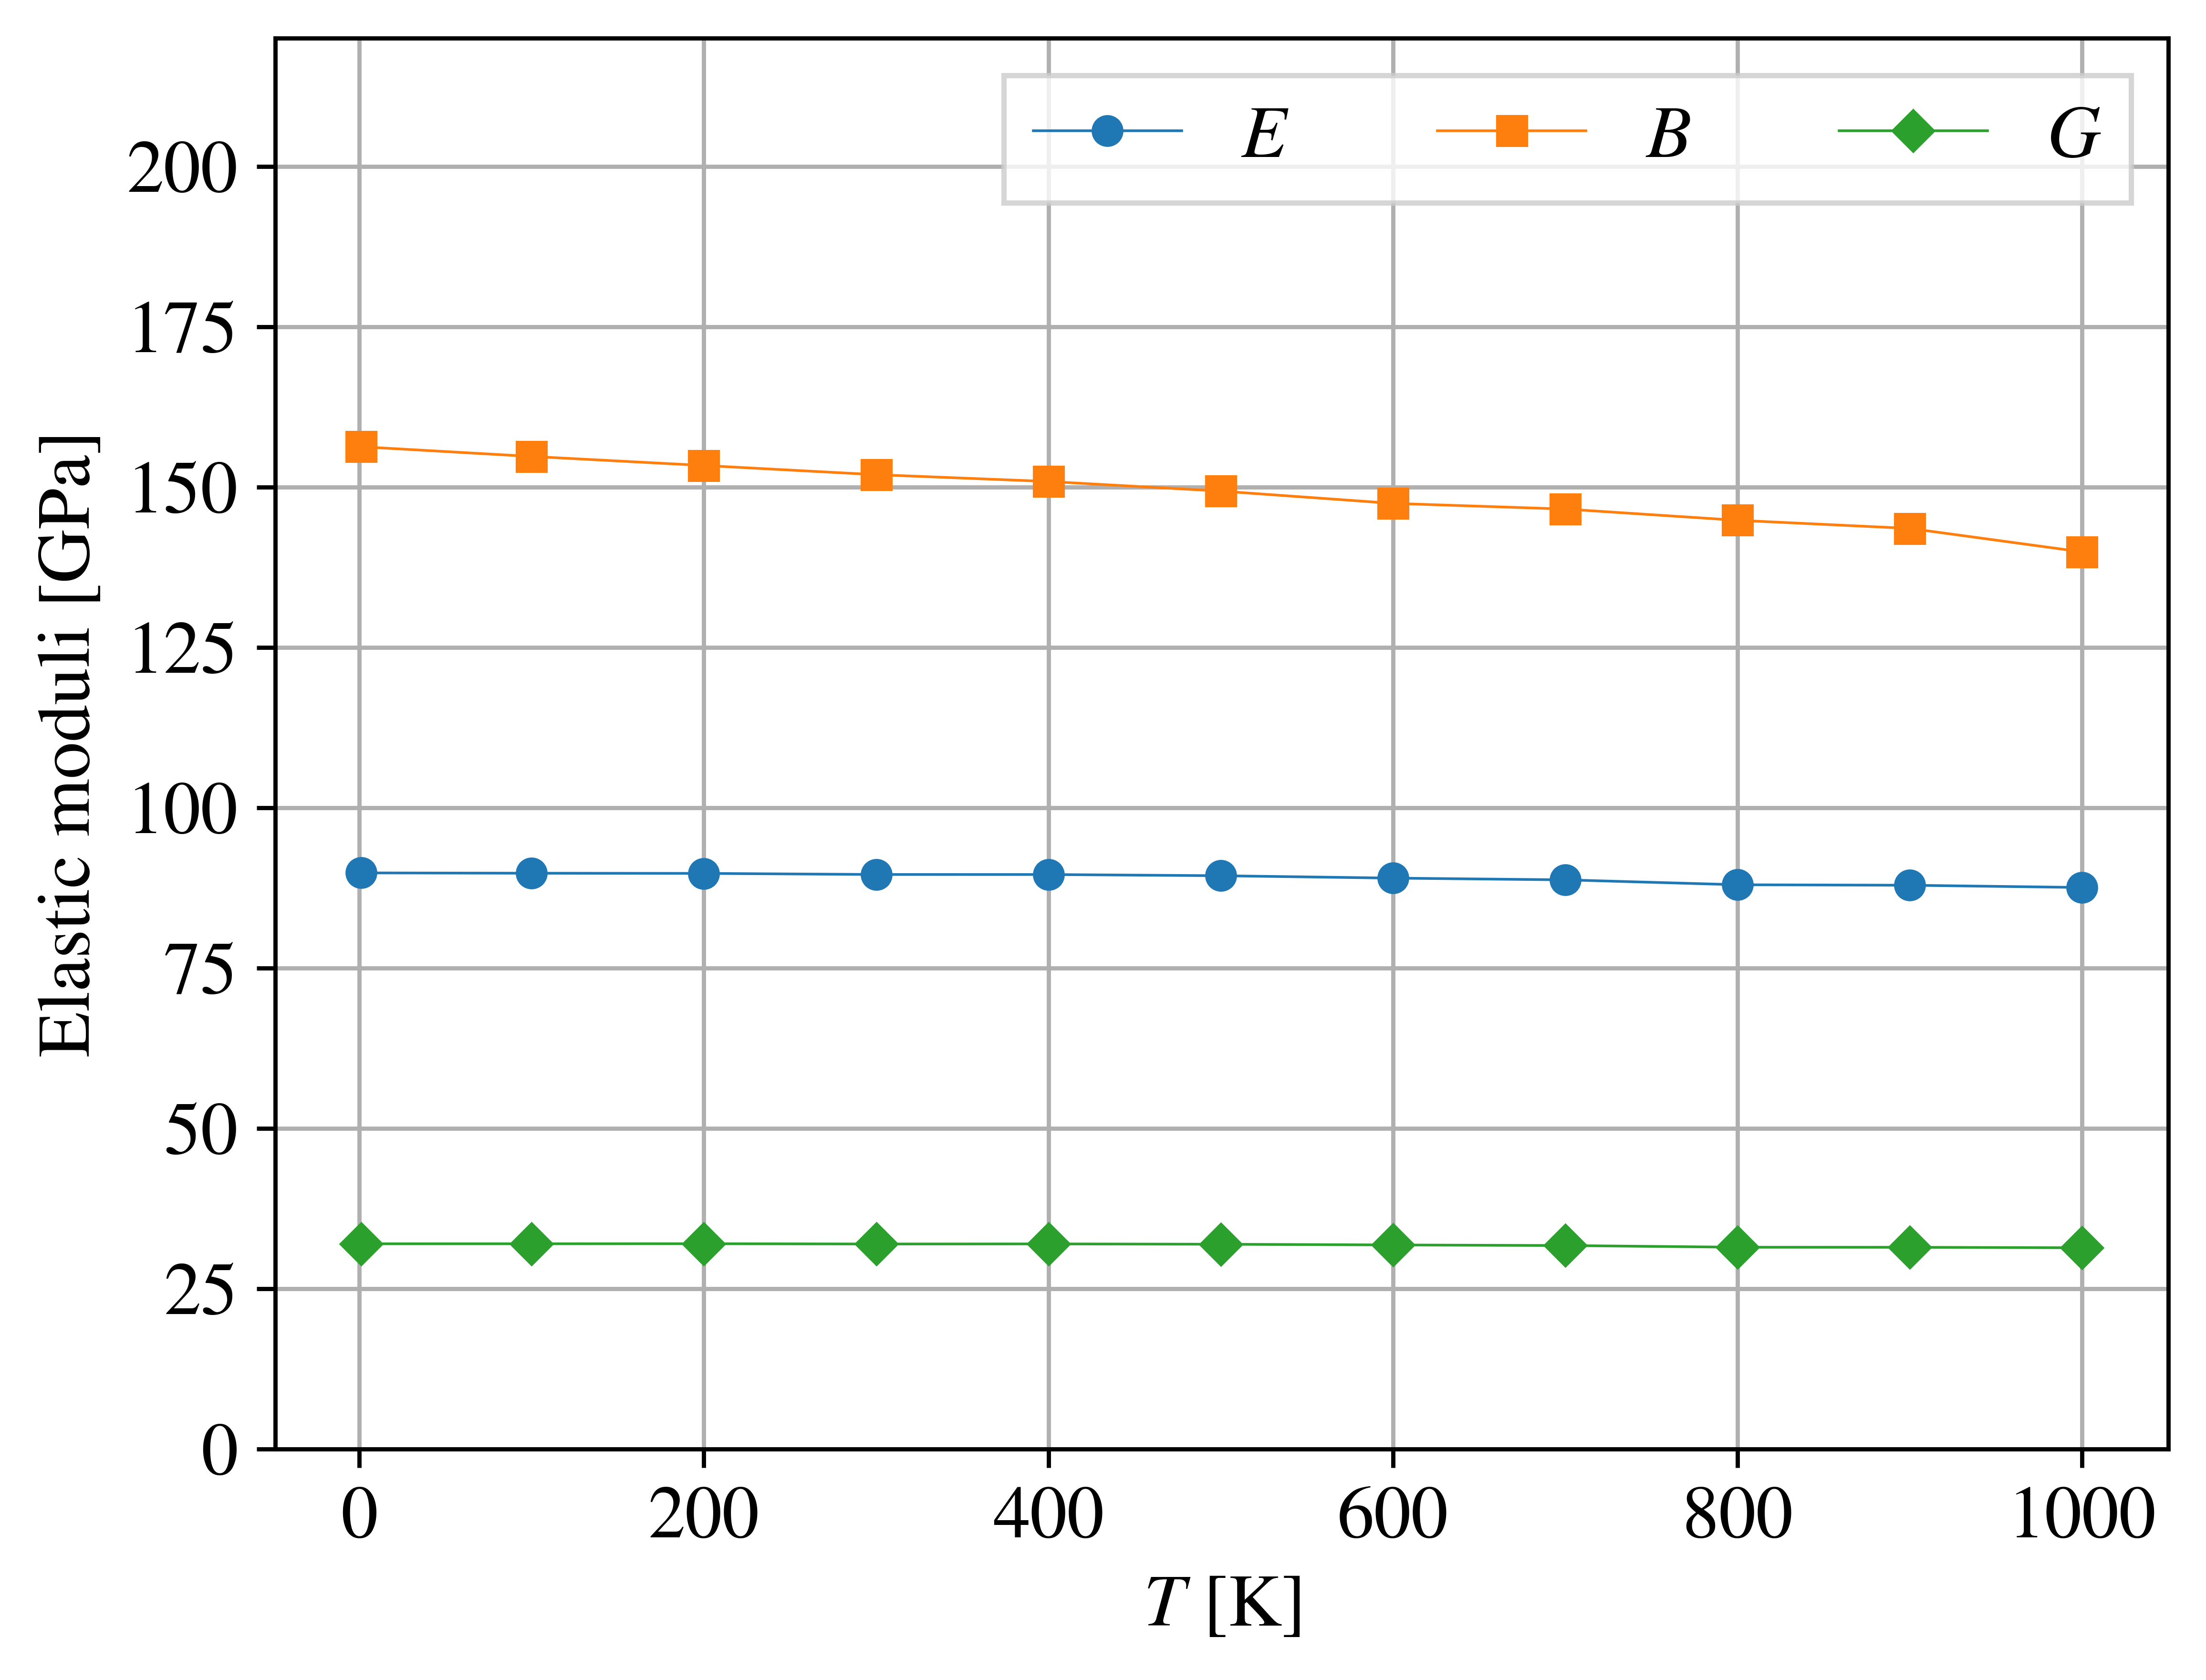
\includegraphics[width=\textwidth]{ElasticModuliaU2N3.png}
    \caption{}
    \label{Fig:ElasModaU2N3}
\end{subfigure}
\hfill
% \begin{subfigure}{0.45\textwidth}
%    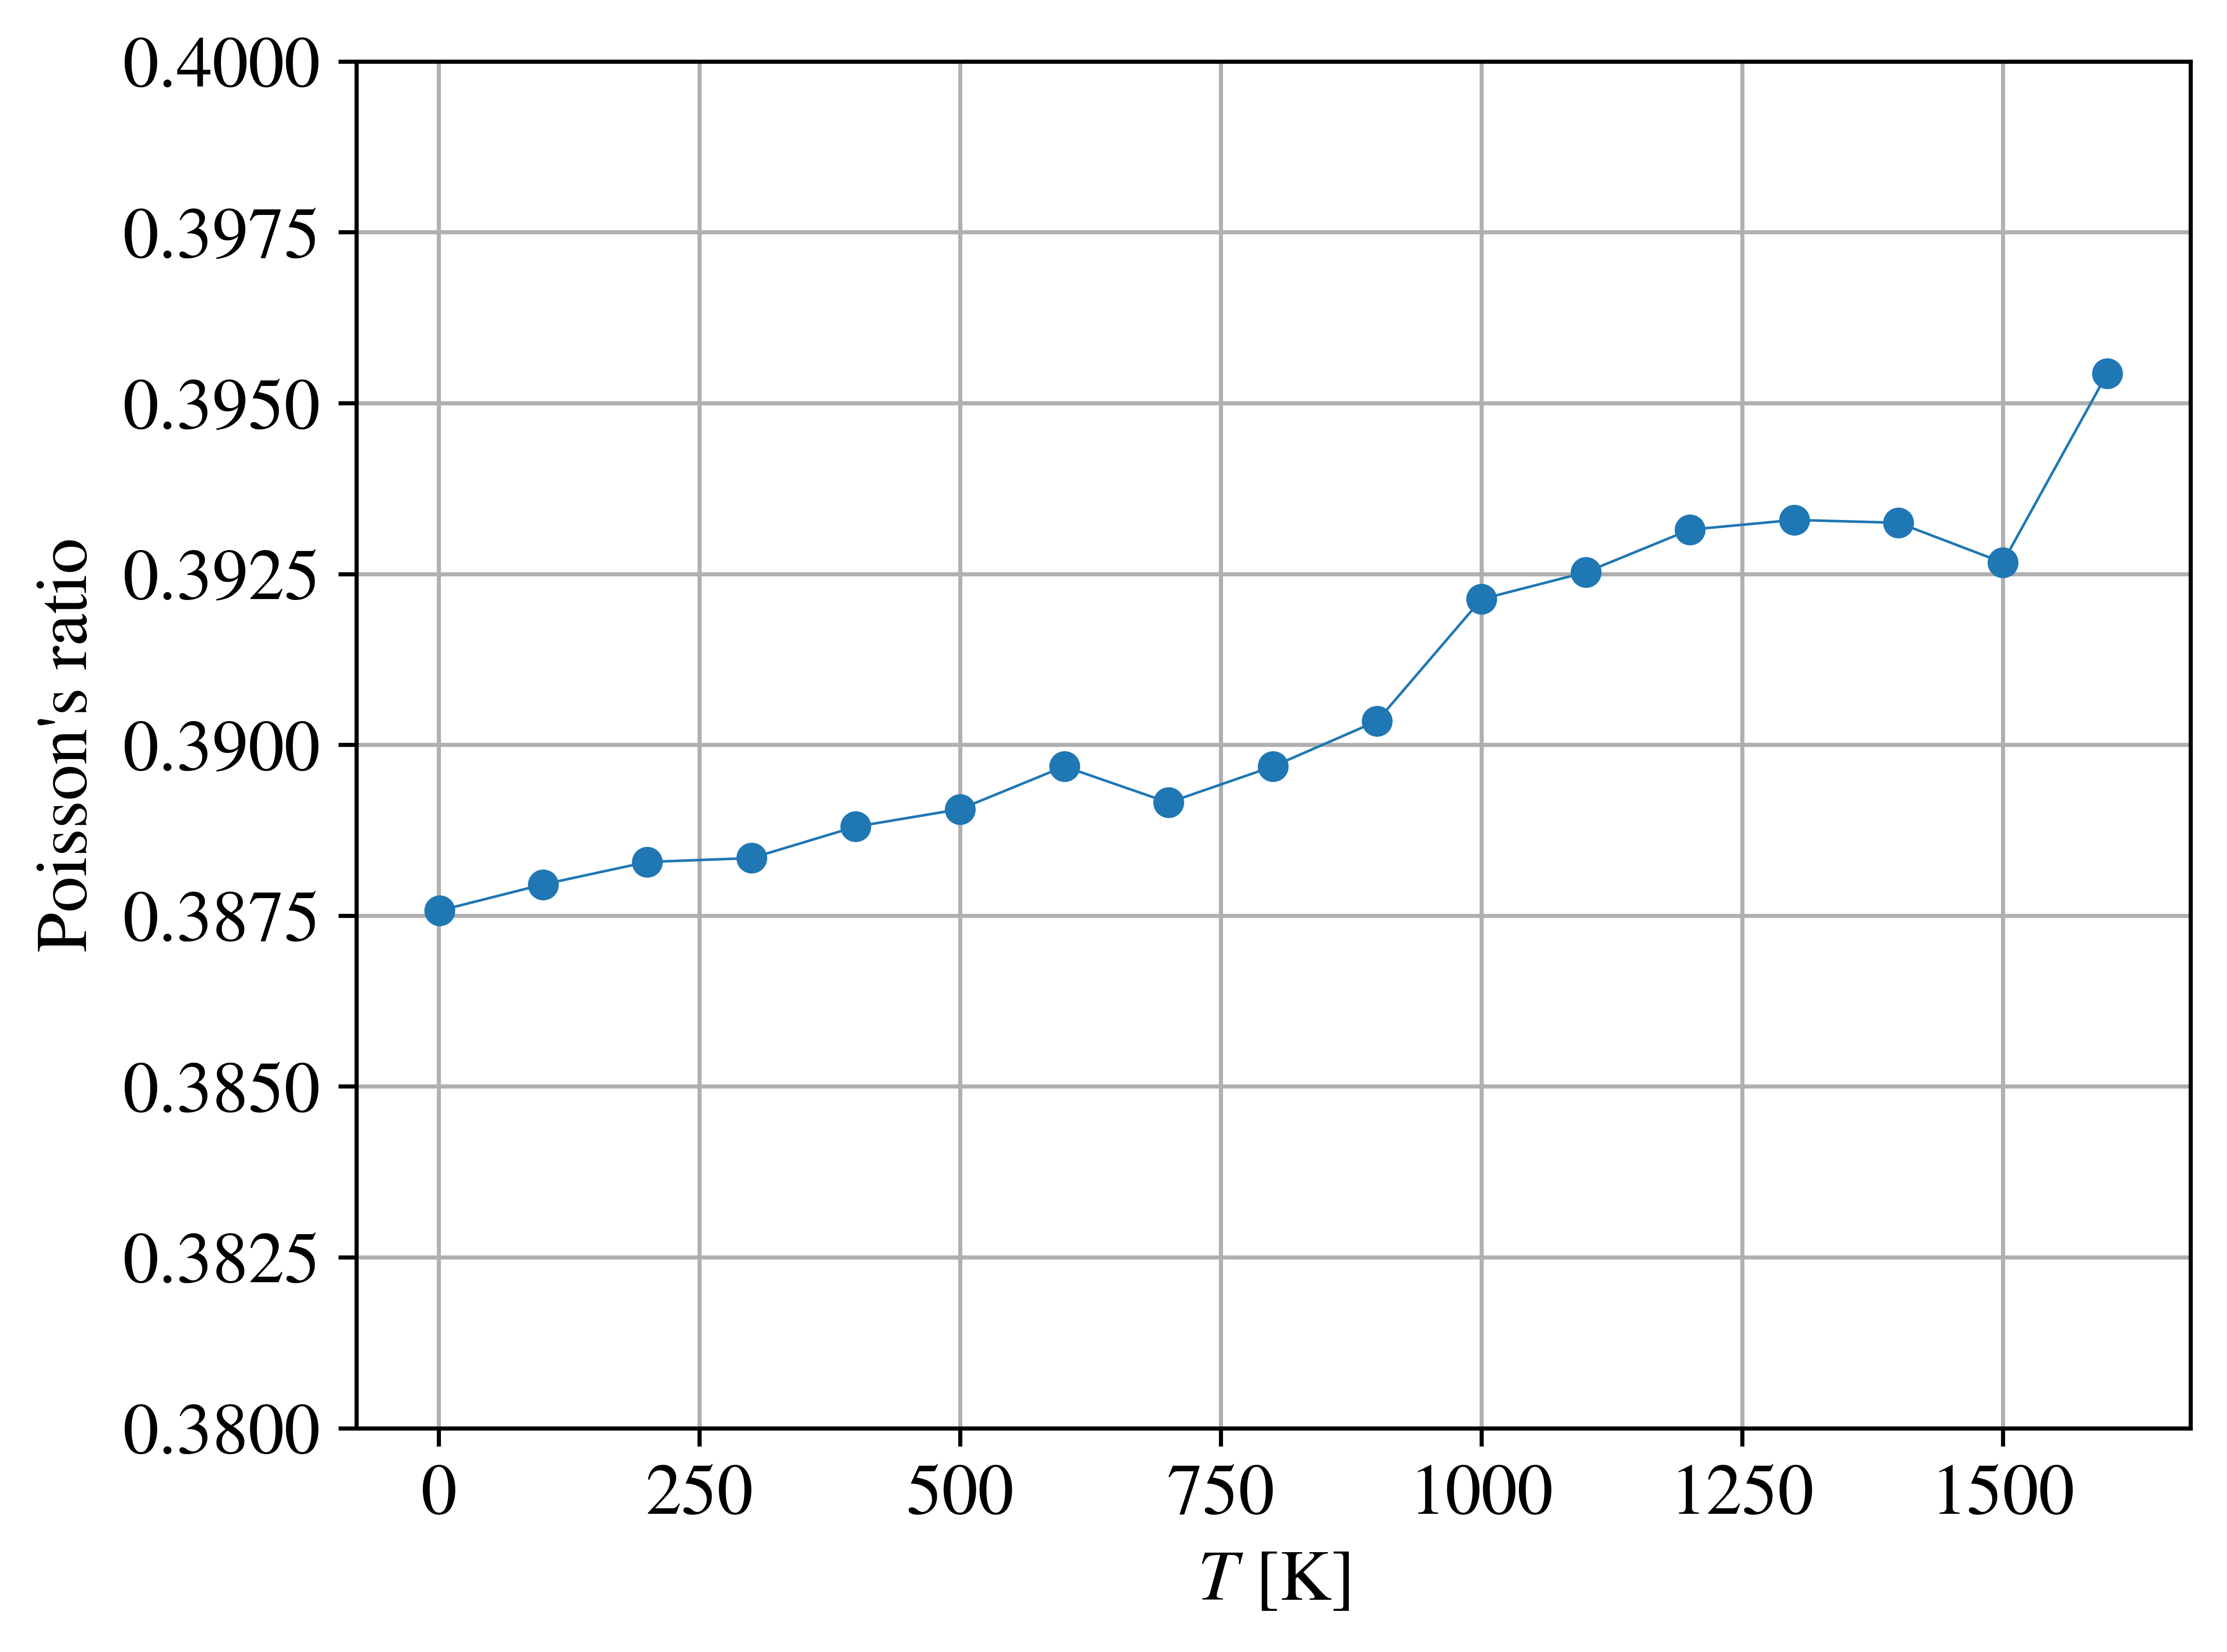
\includegraphics[width=\textwidth]{PoissonRatioU2N3.png}
%    \caption{}
%    \label{Fig:PoissonU2N3}
% \end{subfigure}
\caption{\textbf{(a)} Elastic constants, $C_{11}$, $C_{12}$, and $C_{44}$, \textbf{(b)} Young's modulus, $E$, bulk modulus, $B$, and shear modulus, $G$, of $\alpha$-\ce{U2N3} as calculated by the Kocevski potential.}
% and \textbf{(c)} Poisson's ratio of \ce{U2N3} as calculated by the EAM potential.}
\label{Fig:ECaU2N3}
\end{figure}

\begin{figure}[h!]
\centering
\begin{subfigure}{0.43\textwidth}
    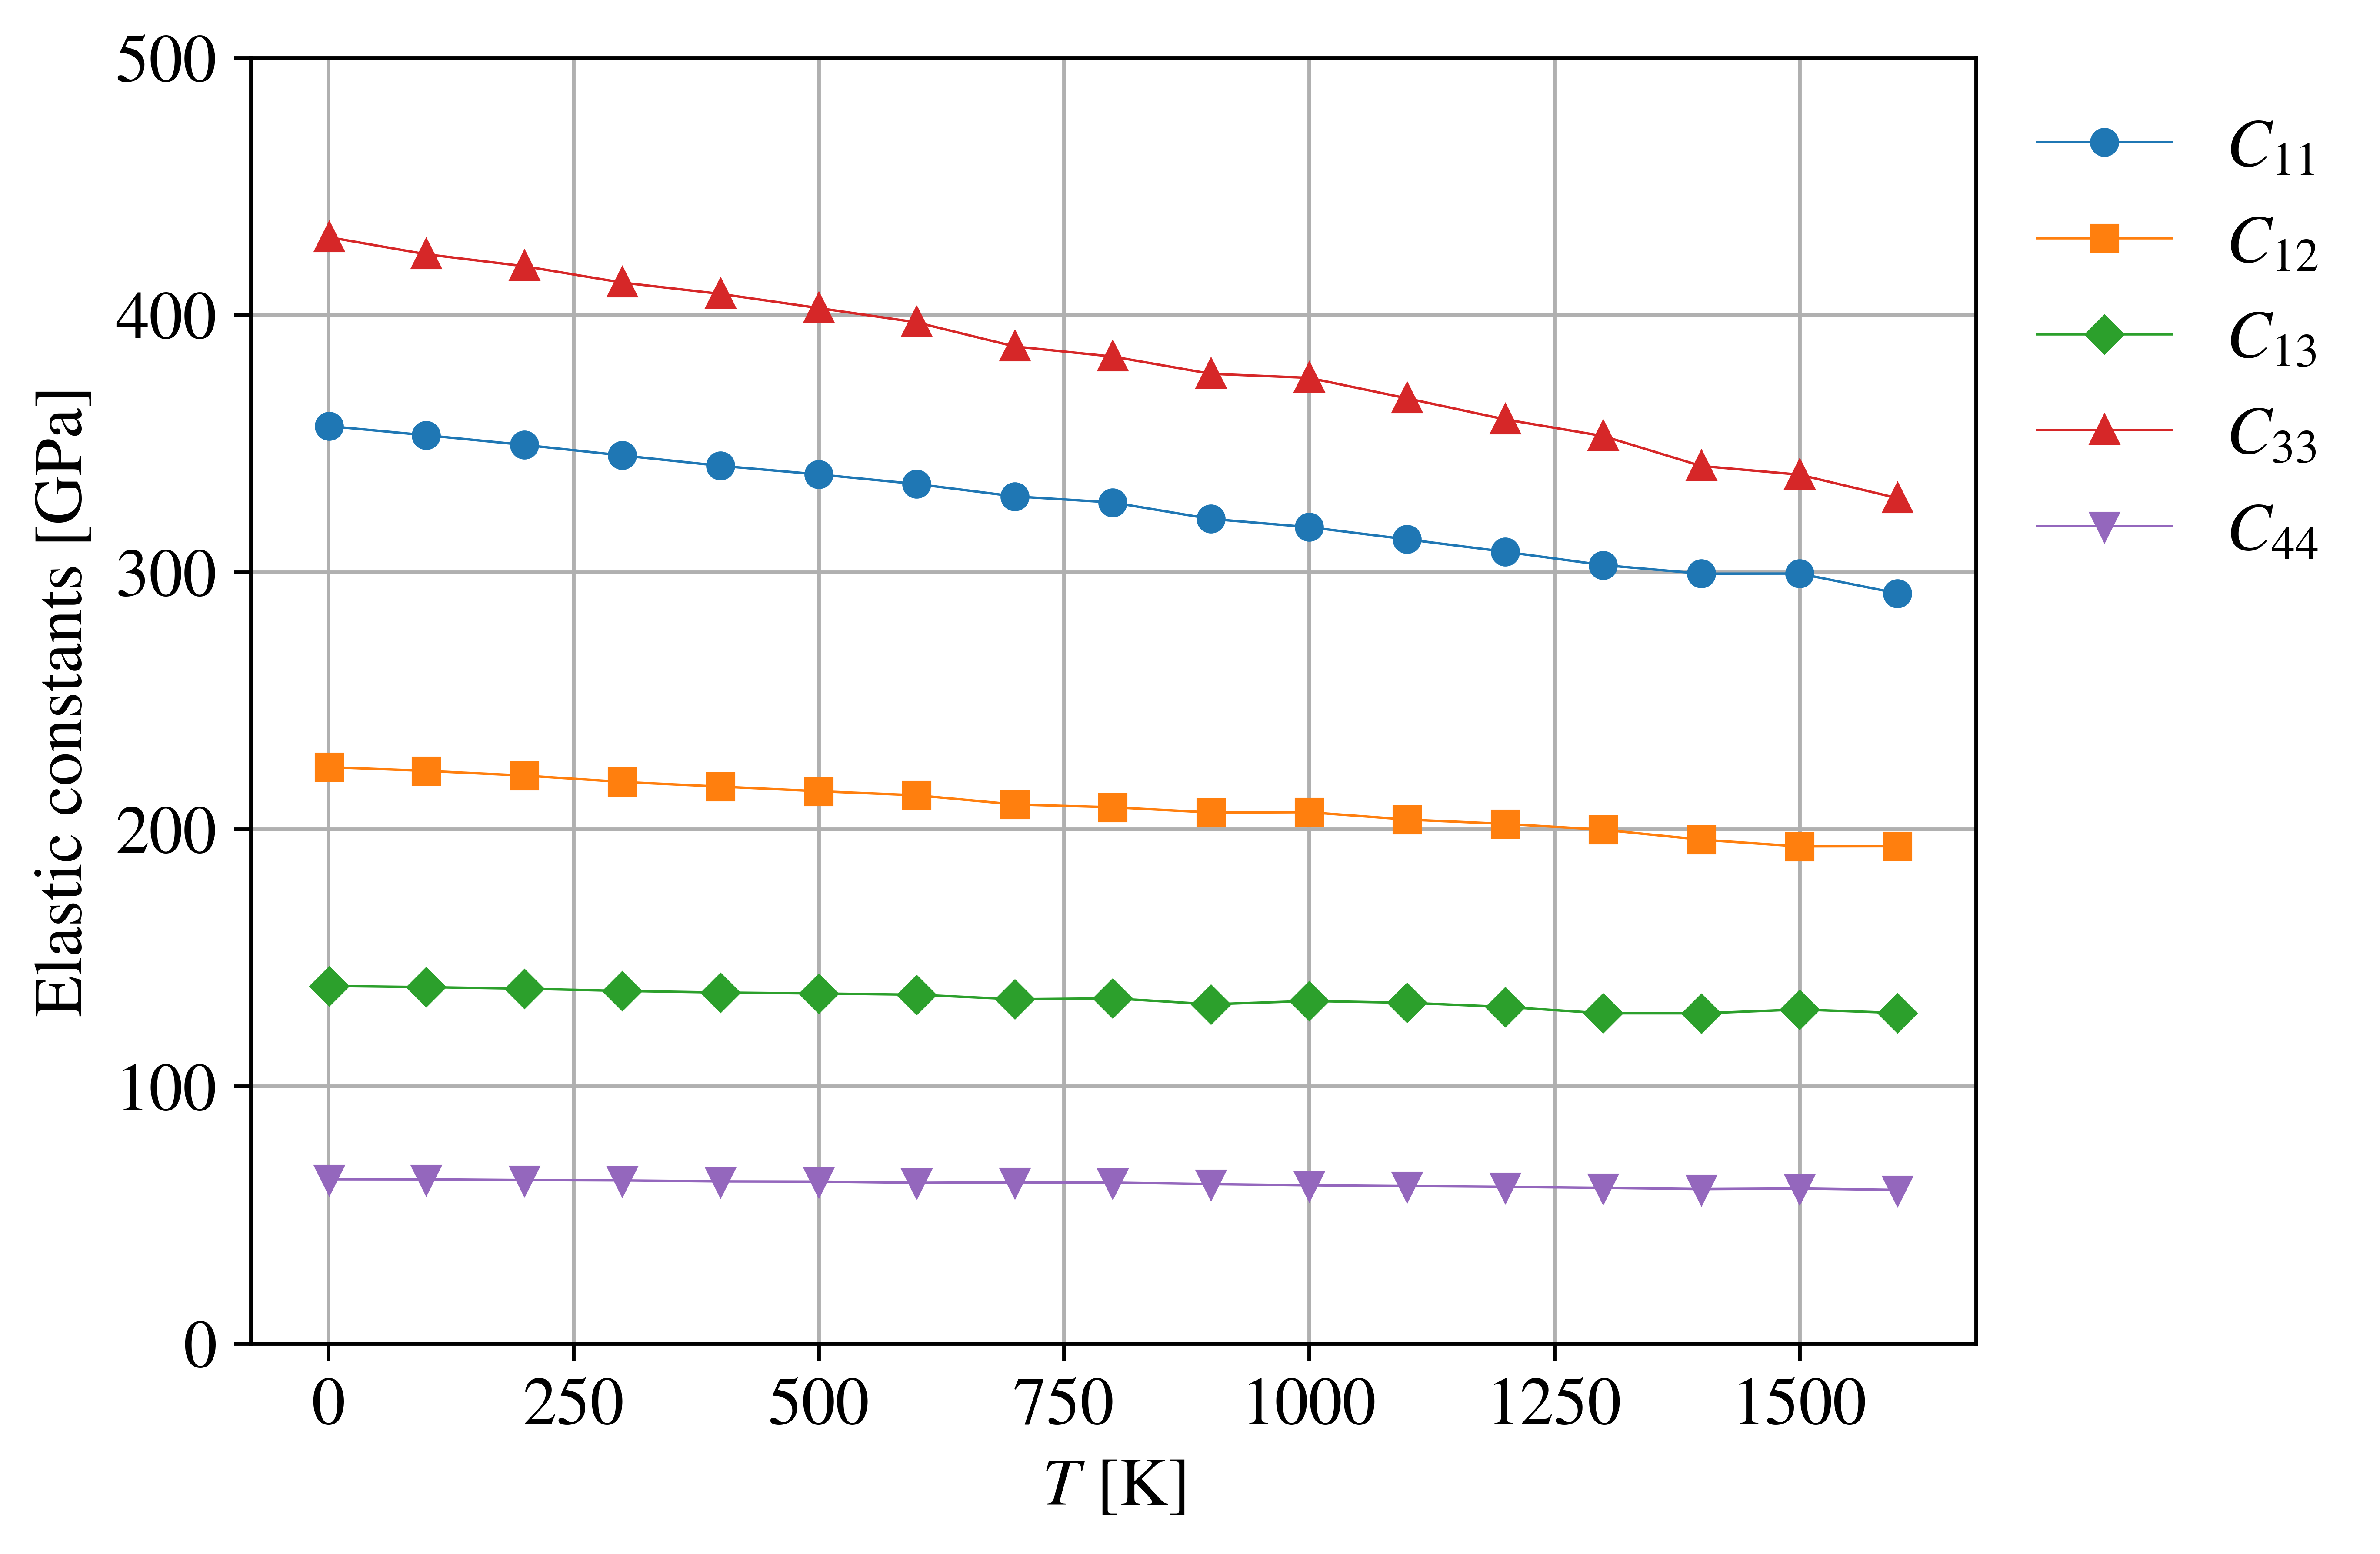
\includegraphics[width=\textwidth]{ElasticConstantsU2N3.png}
    \caption{}
    \label{Fig:ElasConstU2N3}
\end{subfigure}
\hfill
\begin{subfigure}{0.47\textwidth}
    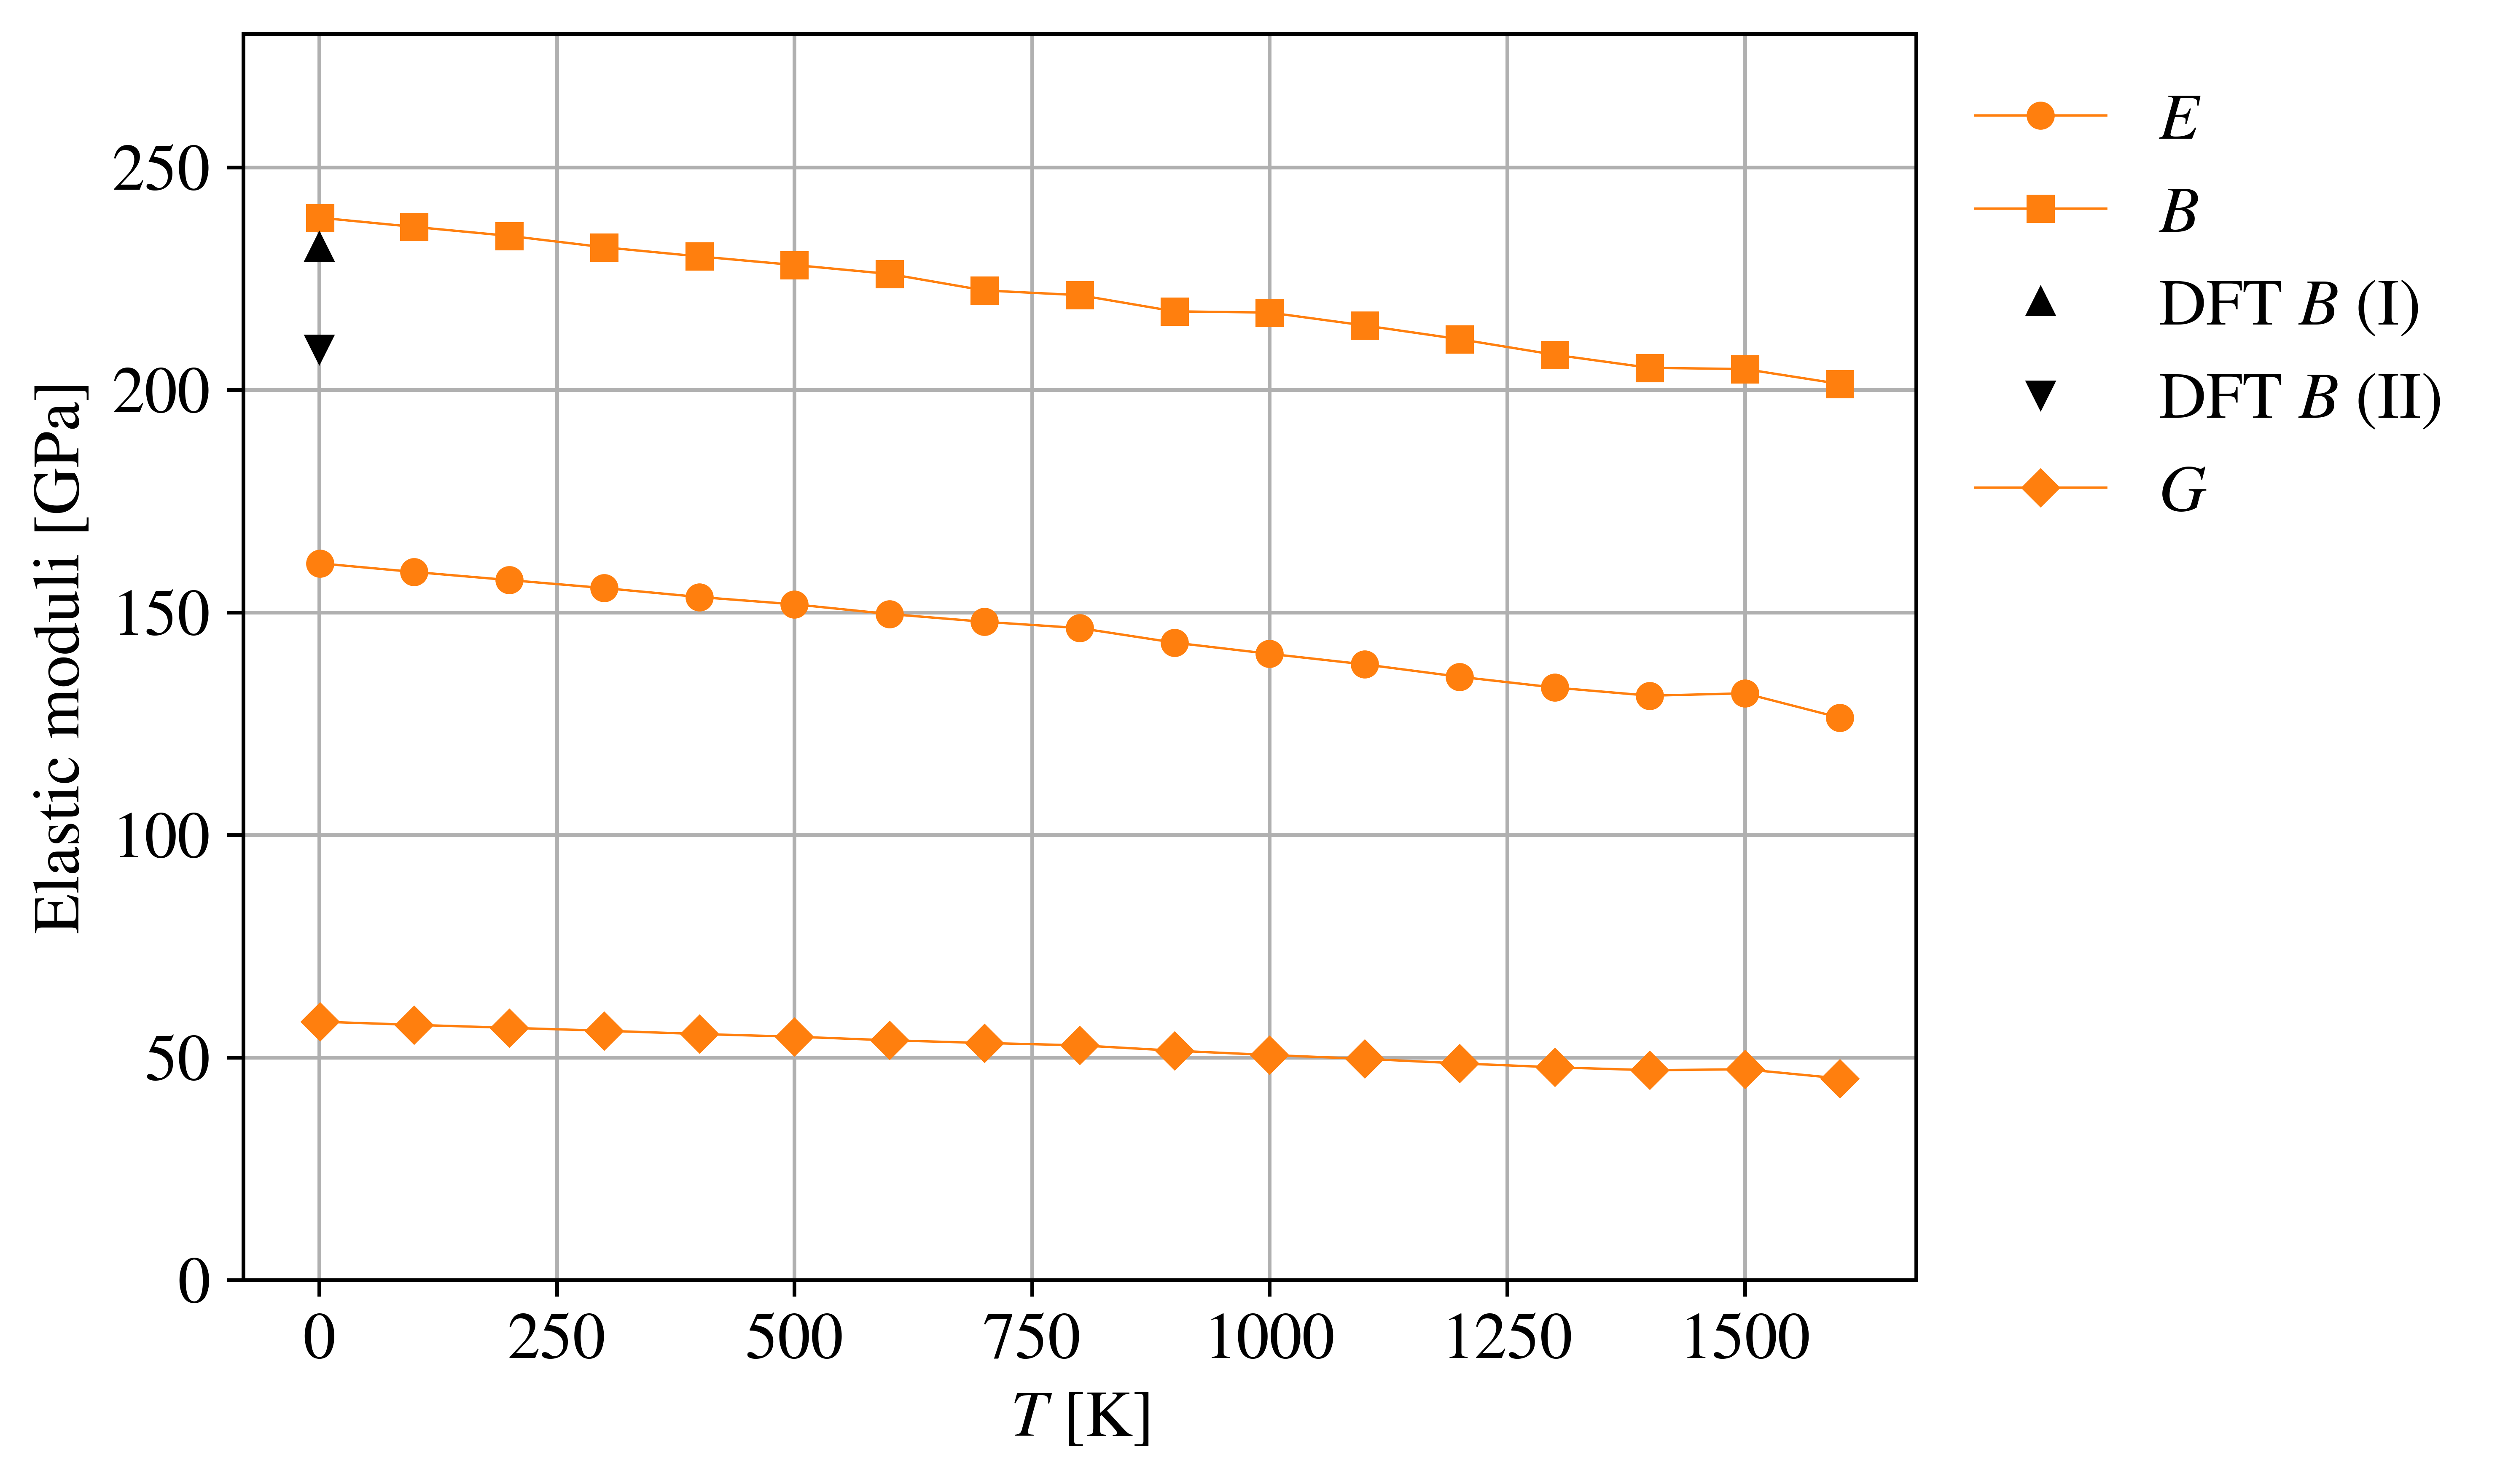
\includegraphics[width=\textwidth]{ElasticModuliU2N3.png}
    \caption{}
    \label{Fig:ElasModU2N3}
\end{subfigure}
\hfill
% \begin{subfigure}{0.45\textwidth}
%    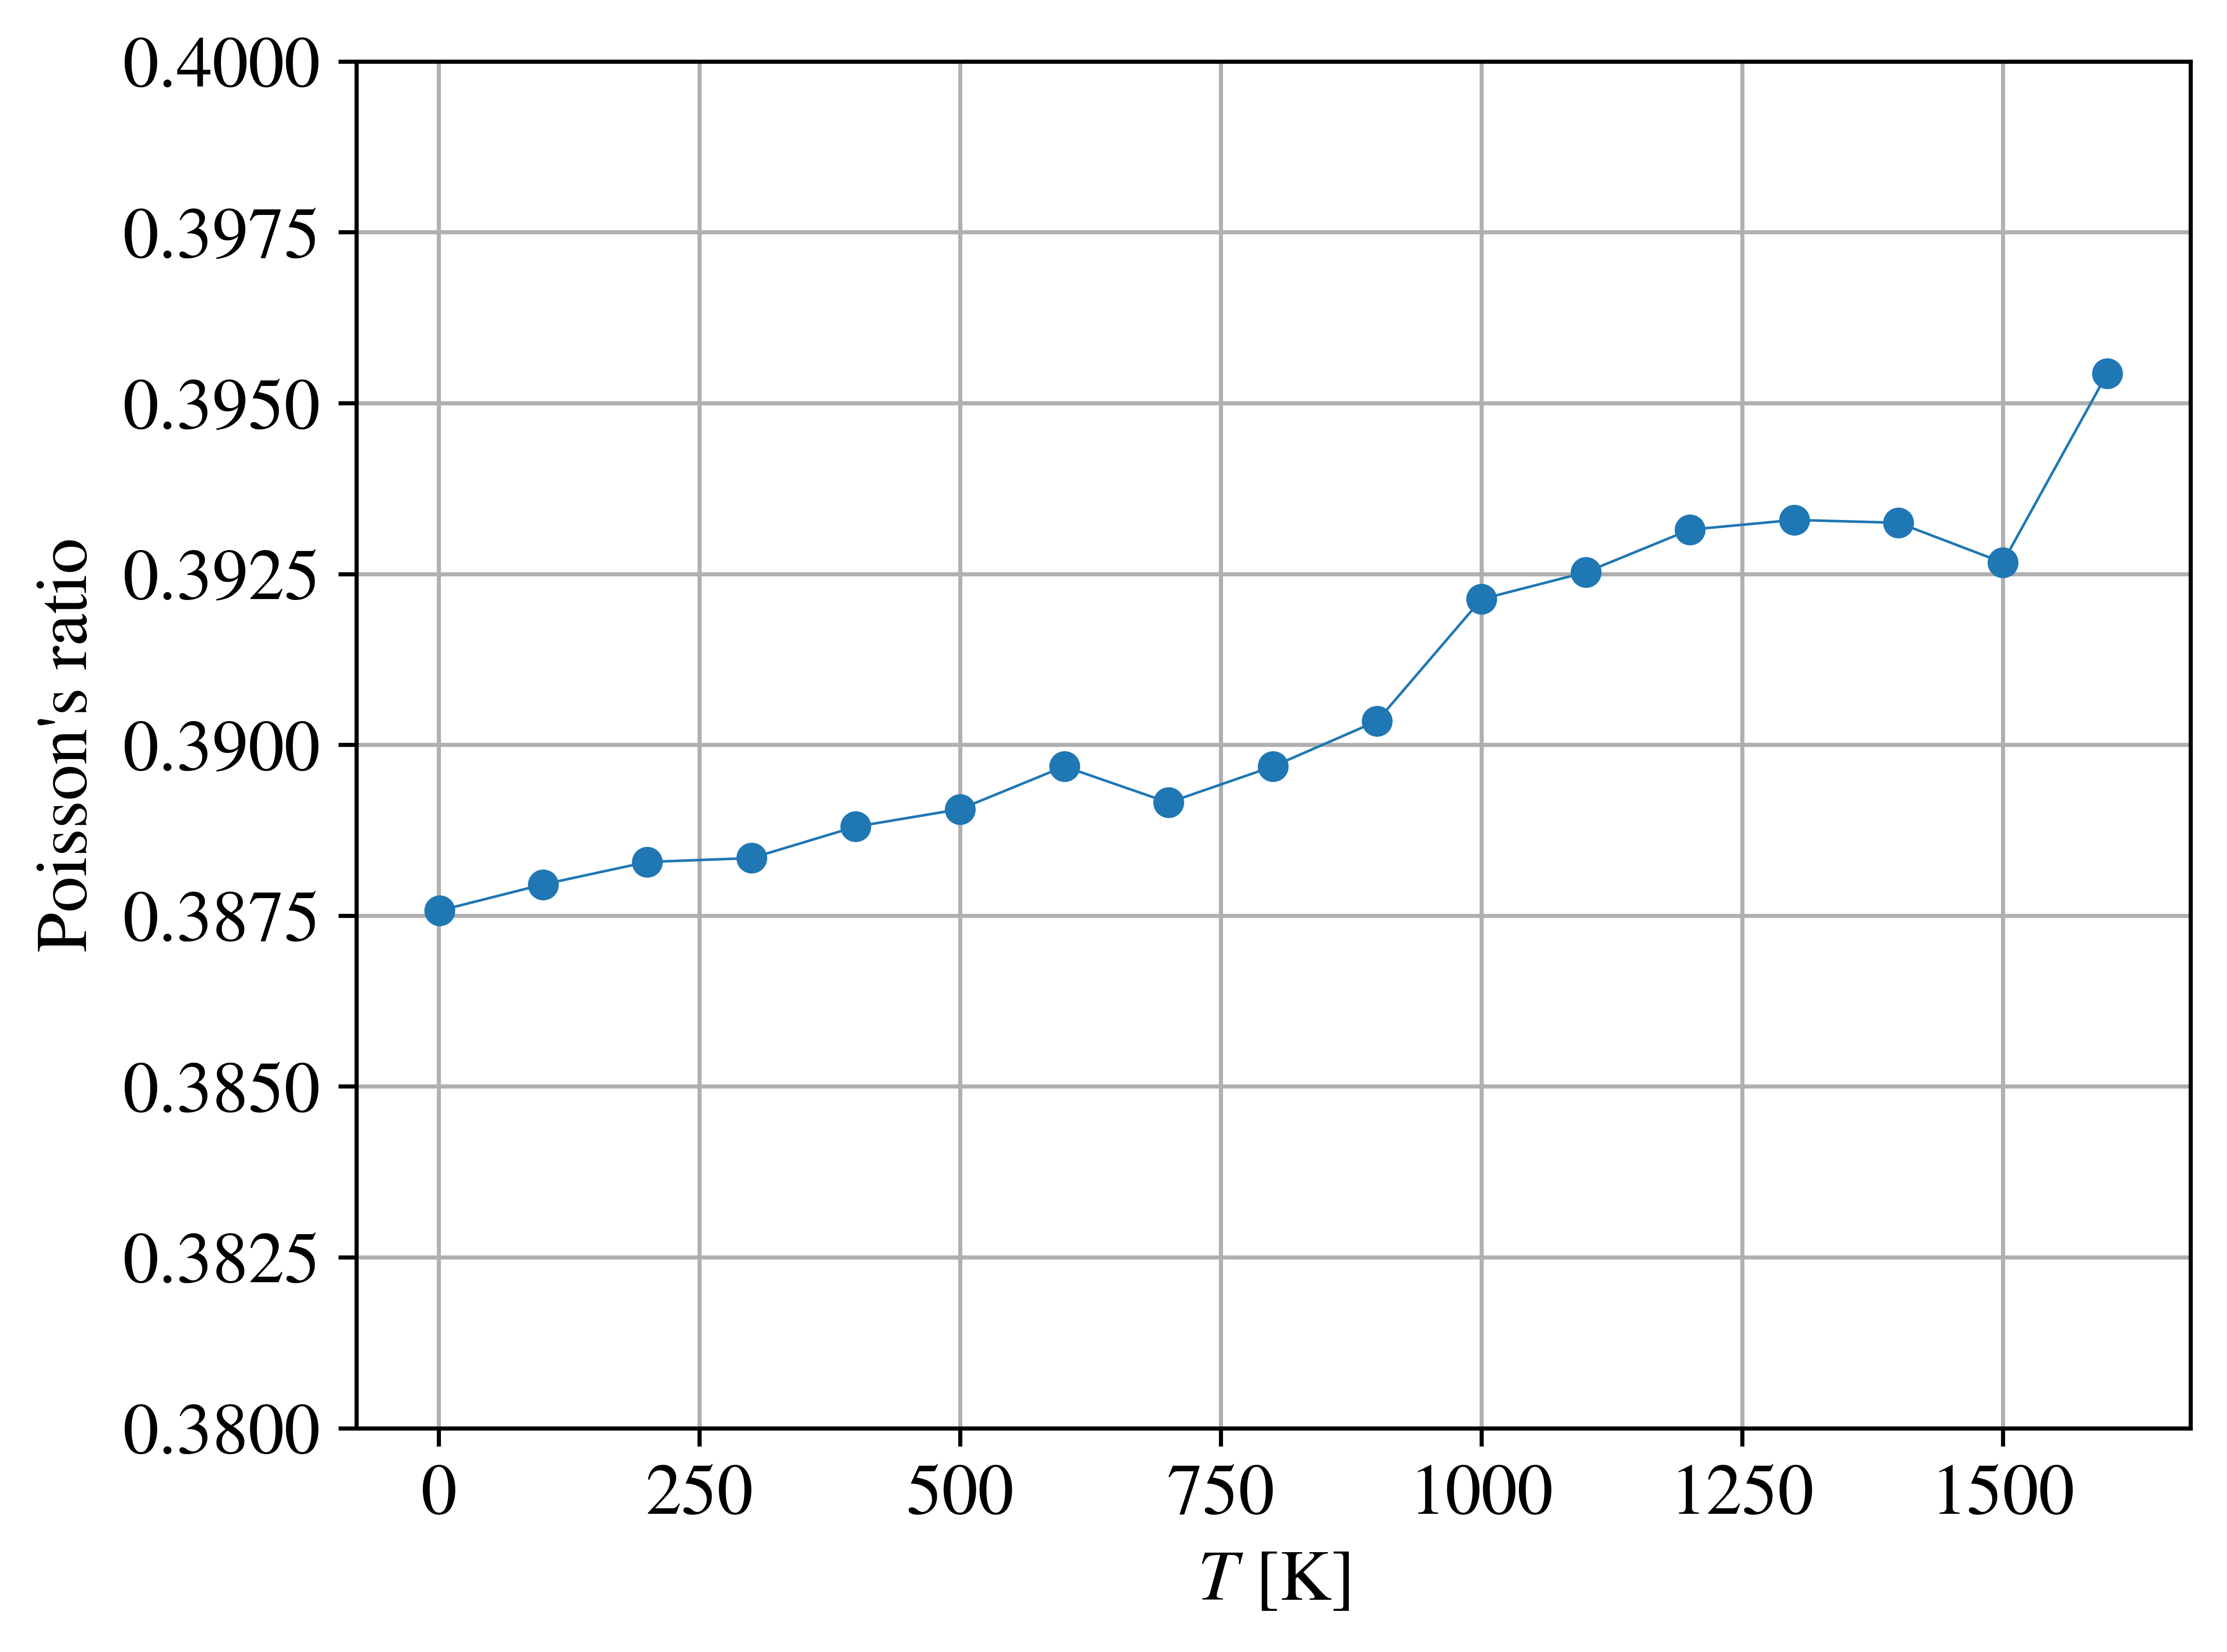
\includegraphics[width=\textwidth]{PoissonRatioU2N3.png}
%    \caption{}
%    \label{Fig:PoissonU2N3}
% \end{subfigure}
\caption{\textbf{(a)} Elastic constants, $C_{11}$, $C_{12}$, $C_{13}$, $C_{33}$, and $C_{44}$, \textbf{(b)} Young's modulus, $E$, bulk modulus, $B$, and shear modulus, $G$, of $\beta$-\ce{U2N3} as calculated by the Kocevski potential. DFT $B$ (I) is from Evarestov \textit{et al.} \cite{Evarestov2008} and DFT $B$ (II) is from Lu \textit{et al.} \cite{Lu2011}.}
% and \textbf{(c)} Poisson's ratio of \ce{U2N3} as calculated by the EAM potential.}
\label{Fig:ECU2N3}
\end{figure}



\section{Discussion}

Based on the presented results, we can identify several features of both potentials. In general, the Kocevski potential shows better predictability of the structural aspects of UN, e.g., lattice parameter and elastic properties as a function of temperature, whereas the Tseplyaev potential better predicts the UN energetic aspects, e.g., the specific heat and defect formation energies. One drawback of the Kocevski potential is the overestimation of the UN optical phonon range, leading to its underestimation of the UN $C_P$, compared to the Hayes \textit{et al.} \cite{Hayes1990IV} correlation, at temperatures greater than 1200 K. Moreover, the Kocevski potential cannot predict a stable metallic $\alpha$-U structure. Therefore, its applicability to studies related to UN non-stoichiometry is limited. The Tseplyaev potential does an inferior job of predicting the UN elastic properties and underpredicts the experimental lattice parameter values compared to the Kocevski potential. The Tseplyaev potential predicts with reasonable accuracy the UN phonon band structure, although the predicted optical branches coincide near the $\Gamma$-point due to the absence of long-range electrostatic interactions in the ADP model. The relative accuracy of the phonon behavior predicted by the Tseplyaev potential should make it preferable in the evaluation of thermal conductivities. Another important feature of the Tseplyaev potential is that it predicts metastable states for defected UN supercells at 0 K, and thus we recommend avoiding its usage at 0 K. Thus, each potential has realms of applicability for the description of the UN system, and the noted drawbacks must be acknowledged when deciding which potential to utilize. 

The predictions of \ce{UN2} properties by the Kocevski potential show better qualitative agreement with the limited experimental and DFT values; however, neither potential produces results with a satisfactory level of accuracy. The Tseplyaev potential cannot predict stable structures for $\alpha$- and $\beta$-\ce{U2N3} and predicts premature phase change of both UN and \ce{UN2}. Thus, the Tseplyaev potential is not suitable for studies related to the stability of different uranium nitride phases. On the other hand, the Kocevski potential predicts stable $\alpha$- and $\beta$-\ce{U2N3} structures with reasonable lattice parameters, reasonably predicts the melting point of UN and predicts a mechanical stability range of \ce{UN2} closer to that represented by the U-N system phase diagrams. This makes the Kocevski potential the best option for studies involving many uranium nitride phases, although more experimental data are needed to further assess its predictions of \ce{UN2}, and $\alpha$- and $\beta$-\ce{U2N3} properties.

% The contradiction in the experimental UN $\theta_D$ is attributed to differences in the formulas used to estimate the average sound velocity and the antiferromagnetic nature of UN below its Néel temperature of 53 K \cite{Samsel2007} which leads to smaller $\theta_D$ values when estimated from specific heat data.

Areas of importance that have not been assessed in this study include the dynamical processes of plastic deformation, i.e., dislocation formation and slip, interfacial properties, and radiation damage. Such analyses are beyond the scope of this work, but potential comparison and validation should be conducted before utilization of either potential to explore these phenomena. 

% The ability of an interatomic potential to model the dynamical processes of plastic deformation, i.e., dislocation formation and slip, must also be assessed by studying the stress-strain behavior of single crystals as the first step to quantifying such behavior. This study is beyond the scope of the current research paper and is the subject of our future work.

\section{Conclusions}

This work aimed to evaluate two UN interatomic potentials: Tseplyaev and Starikov's ADP \cite{Tseplyaev2016} and Kocevski \textit{et al.}'s EAM potential \cite{Kocevski2022II}. The study involved assessing the predictive capabilities of these potentials for various thermophysical and elastic properties of UN, \ce{UN2}, and $\alpha$- and $\beta$-\ce{U2N3}. The Kocevski potential underestimates the UN specific heat which is attributed to its overestimation of the UN optical phonon frequency range. In terms of performance, the Tseplyaev potential excels in capturing the energetic aspects of UN, whereas the Kocevski potential performs better in modeling the UN's structural properties. Regarding the mechanical stability of phases, the Kocevski potential demonstrates superior predictive capabilities, in that it can reasonably estimate the UN melting point and predicts stable $\alpha$- and $\beta$-\ce{U2N3} structures. In contrast, the Tseplyaev potential predicts premature phase changes for both UN and \ce{UN2} and fails to stabilize either polymorph of \ce{U2N3}. An important limitation of the Kocevski potential is its inability to predict a stable metallic U phase, making it unsuitable for studies related to UN non-stoichiometry.

\section*{Acknowledgements}

The authors would like to thank Antoine Claisse for the fruitful discussions. Mohamed AbdulHameed dedicates this work to the memory of Abu Bakr Etman. This research made use of the resources of the High-Performance Computing Center at Idaho National Laboratory, which is supported by the Office of Nuclear Energy of the U.S. Department of Energy and the Nuclear Science User Facilities under Contract No. DE-AC07-05ID14517.

\appendix

\section{Voigt-Reuss-Hill elastic moduli}
\label{appelas}
For an isotropic polycrystalline material with a cubic crystal structure, the form of the VRH elastic moduli is \cite{Anderson1963, Rosler2007}:
\begin{equation}
B = B_V = B_R = \frac{C_{11} + 2 C_{12}}{3}
\label{Eq:KV}
\end{equation}

\begin{equation}
G_V = \frac{C_{11}-C_{12}+3C_{44}}{5}
\label{Eq:GV}
\end{equation}

\begin{equation}
G_R = \frac{5 C_{44} \left( C_{11}-C_{12} \right) }{4 C_{44} + 3 \left( C_{11}-C_{12} \right)}
\label{Eq:GR}
\end{equation}

\begin{equation}
G = \frac{G_V + G_R}{2}
\end{equation}

\begin{equation}
E = \frac{9BG}{3B+G}
\end{equation}

\begin{equation}
\nu = \frac{3B-2G}{6B+2G}
\end{equation}

For the $\beta$-\ce{U2N3} hexagonal crystal, the Voigt and Reuss limits on the bulk and shear moduli are formulated in terms of the components of both the stiffness tensor, $C_{ij}$, and the compliance tensor, $S_{ij}$ \cite{Anderson1963, Rosinger1979}:
\begin{equation}
B_V = \frac{2 C_{11} + 2 C_{12} + 4 C_{13} + C_{33}}{9}
\end{equation}
\begin{equation}
B_R = \frac{1}{2 S_{11} + 2 S_{12} + 4 S_{13} + S_{33}}
\end{equation}
\begin{equation}
B = \frac{B_V + B_R}{2}
\end{equation}
\begin{equation}
G_V = \frac{2 C_{11} - C_{12} - 2 C_{13} + C_{33} + 6 C_{44} + 3 C_{66}}{15}
\end{equation}
\begin{equation}
G_R = \frac{15}{8 S_{11} - 4 S_{12} - 8 S_{13} + 4 S_{33} + 6 S_{44} + 3 S_{66}}
\end{equation}
where $S_{11}$, $S_{12}$, $S_{13}$, $S_{33}$, and $S_{44}$ are the independent components of the compliance tensor, and:
\begin{equation}
S_{11} = \frac{C_{11} C_{33} - C_{13}^2}{C_{11} \left( C_{11} C_{33} - 2 C_{13}^2 \right) - C_{12} \left( C_{12} C_{33} + 2 C_{13}^2 \right)}
\end{equation}
\begin{equation}
S_{12} = \frac{- C_{12} C_{33} + C_{13}^2}{C_{11} \left( C_{11} C_{33} - 2 C_{13}^2 \right) - C_{12} \left( C_{12} C_{33} + 2 C_{13}^2 \right)}
\end{equation}
\begin{equation}
S_{13} = \frac{-C_{13}}{C_{33} \left( C_{11}+C_{12} \right) - 2 C_{13}^2}
\end{equation}
\begin{equation}
S_{33} = \frac{C_{11} + C_{12}}{C_{33} \left( C_{11}+C_{12} \right) - 2 C_{13}^2}
\end{equation}
\begin{equation}
S_{44} = \frac{1}{C_{44}}
\end{equation}
\begin{equation}
C_{66} = \frac{C_{11} - C_{12}}{2}
\end{equation}
\begin{equation}
S_{66} = 2 (S_{11} - S_{12})
\end{equation}

\section{Supplementary information}
\label{app}

In all equations presented in this appendix, the superscript $T$ refers to the Tseplyaev potential and the superscript $K$ refers to the Kocevski potential.

The temperature variation of the LTEC computed by both potentials is fitted to the following functions: 
\begin{equation}
\begin{array}{cc}
\alpha_L^T = 7.321 \times 10^{-6} - 3.063 \times 10^{-11} T + 2.154 \times 10^{23} T^5 & \left( R^2 = 99.8\% \right)
\end{array}
\label{Eq:LTEC1}
\end{equation}
\begin{equation}
\begin{array}{cc}
\alpha_L^{K} = 5.773 \times 10^{-6} + 3.866 \times 10^{-10} T + 1.813 \times 10^{-13} T^2 & \left( R^2 = 99.9\% \right)
\end{array}
\label{Eq:LTEC2}
\end{equation}
in the temperature range 50-2500 K.

The temperature dependence of the bulk modulus computed by both potentials is fitted to the following quadratic functions:
\begin{equation}
\begin{array}{cc}
B^T = 275.063 - 3.314 \times 10^{-2} T - 7.649 \times 10^{-6} T^2 & \left( R^2 = 98.4\% \right)
\end{array}
\label{Eq:B1}
\end{equation}
\begin{equation}
\begin{array}{cc}
B^K = 219.196 - 1.955 \times 10^{-2} T - 4.517 \times 10^{-6} T^2 & \left( R^2 = 99.8\% \right)
\end{array}
\label{Eq:B2}
\end{equation}
in the temperature range of 1-2600 K.

The UN $C_P$ and $C_V$ computed by both potentials have been fitted to:
\begin{equation}
\begin{array}{cc}
C_P^T = 61.612 + 4.709 \times 10^{-3} T + 3.754 \times 10^{-16} T^5 - 19.663 / T^{0.1} & \left( R^2 = 99.4\% \right)
\label{CPADP}
\end{array}
\end{equation}

\begin{equation}
\begin{array}{cc}
C_P^K = 50.500 + 6.193 \times 10^{-3} T + 1.272 \times 10^{-13} T^4 - 1.140 / T^{0.1} & \left( R^2 = 99.7\% \right)    
\end{array}
\label{CPEAM}
\end{equation}

\begin{equation}
\begin{array}{cc}
C_V^T = 49.341 + 7.144 \times 10^{-4} T + 4.016 \times 10^{-8} T^{2.5} + 0.591 / T^{0.1} & \left( R^2 = 98.8\% \right)
\label{CVADP}
\end{array}
\end{equation}

\begin{equation}
\begin{array}{cc}
C_V^K = 49.978 + 8.757 \times 10^{-4} T + 1.616 \times 10^{-7} T^2 & \left( R^2 = 80.8\% \right)
\label{CVEAM}
\end{array}
\end{equation}

The \ce{UN2} $C_P$ calculated by both potentials are fitted to:
\begin{equation}
\begin{array}{cc}
C_P^T = 54.894 + 1.803 \times 10^{-2} T + 8.717 \times 10^{-15} T^5 + 30.248 / T^{0.1} & \left( R^2 = 98.9\% \right)
\end{array}
\label{CPUN2ADP}
\end{equation}

\begin{equation}
\begin{array}{cc}
C_P^K = 82.060 - 2.445 \times 10^{-3} T + 3.199 \times 10^{-6} T^2 - 10.934 / T^{0.1} & \left( R^2 = 95.1\% \right)
\end{array}
\label{CPUN2EAM}
\end{equation}

whereas the $\alpha$-\ce{U2N3} $C_P$ calculated by the Kocevski potential is fitted to:
\begin{equation}
\begin{array}{cc}
C_P^{K} = 155.092 - 1.686 \times 10^{-2} T + 1.534 \times 10^{-5} T^2 - 45.235 / T^{0.1} & \left( R^2 = 93.3\% \right)
\end{array}
\label{CPU2N3b}
\end{equation}

and the $\beta$-\ce{U2N3} $C_P$ calculated by the Kocevski potential is fitted to:
\begin{equation}
\begin{array}{cc}
C_P^{K} = 132.240 + 7.979 \times 10^{-4} T + 2.544 \times 10^{-6} T^2 - 11.483 / T^{0.1} & \left( R^2 = 91.1\% \right)
\end{array}
\label{CPU2N3}
\end{equation}

\begin{table}[h!]
\centering
\caption{Cohesive energies (eV) of UN, $\alpha$-U and \ce{UN2}.}
\footnotesize
\begin{tabular}{c|c|c|c}
\hline
           & Tseplyaev potential                      & Kocevski potential    & Reference value                           \\
\hline
UN         & -16.18                   & -13.02 & -13.6 (Expt.) \cite{Evarestov2008}        \\
$\alpha$-U & -5.23 (0 K); -5.37 (1 K) & -      & -5.55 (Expt.) \cite{Kittel2005}           \\
\ce{UN2}   & -24.62                   & -22.18 & -21.5 to -17.9 (DFT) \cite{Evarestov2008} \\
\hline
\end{tabular}
\label{Tab:CohesiveE}
\end{table}

\begin{table}[h!]
    \centering
    \caption{U and N chemical potentials (eV) for different stoichiometric conditions.}
    \footnotesize
    \begin{tabular}{c|ccc|c}
    \hline
            & \multicolumn{3}{c|}{Tseplyaev potential}          & Kocevski potential \\
            & U-rich & Stoichiometric & N-rich & N-rich \\
    \hline
    $\mu_U$ & -5.23 (0 K); -5.37 (1 K)   & -6.49 (0 K); -6.56 (1 K) & -7.75 & -3.86 \\
    $\mu_N$ & -10.95 (0 K); -10.81 (1 K) & -9.69 (0 K); -9.62 (1 K) & -8.43 & -9.16 \\
    \hline
    \end{tabular}
    \label{Tab:ChemPot}
\end{table}

\begin{figure}[h!]
\centering
\begin{subfigure}{0.45\textwidth}
    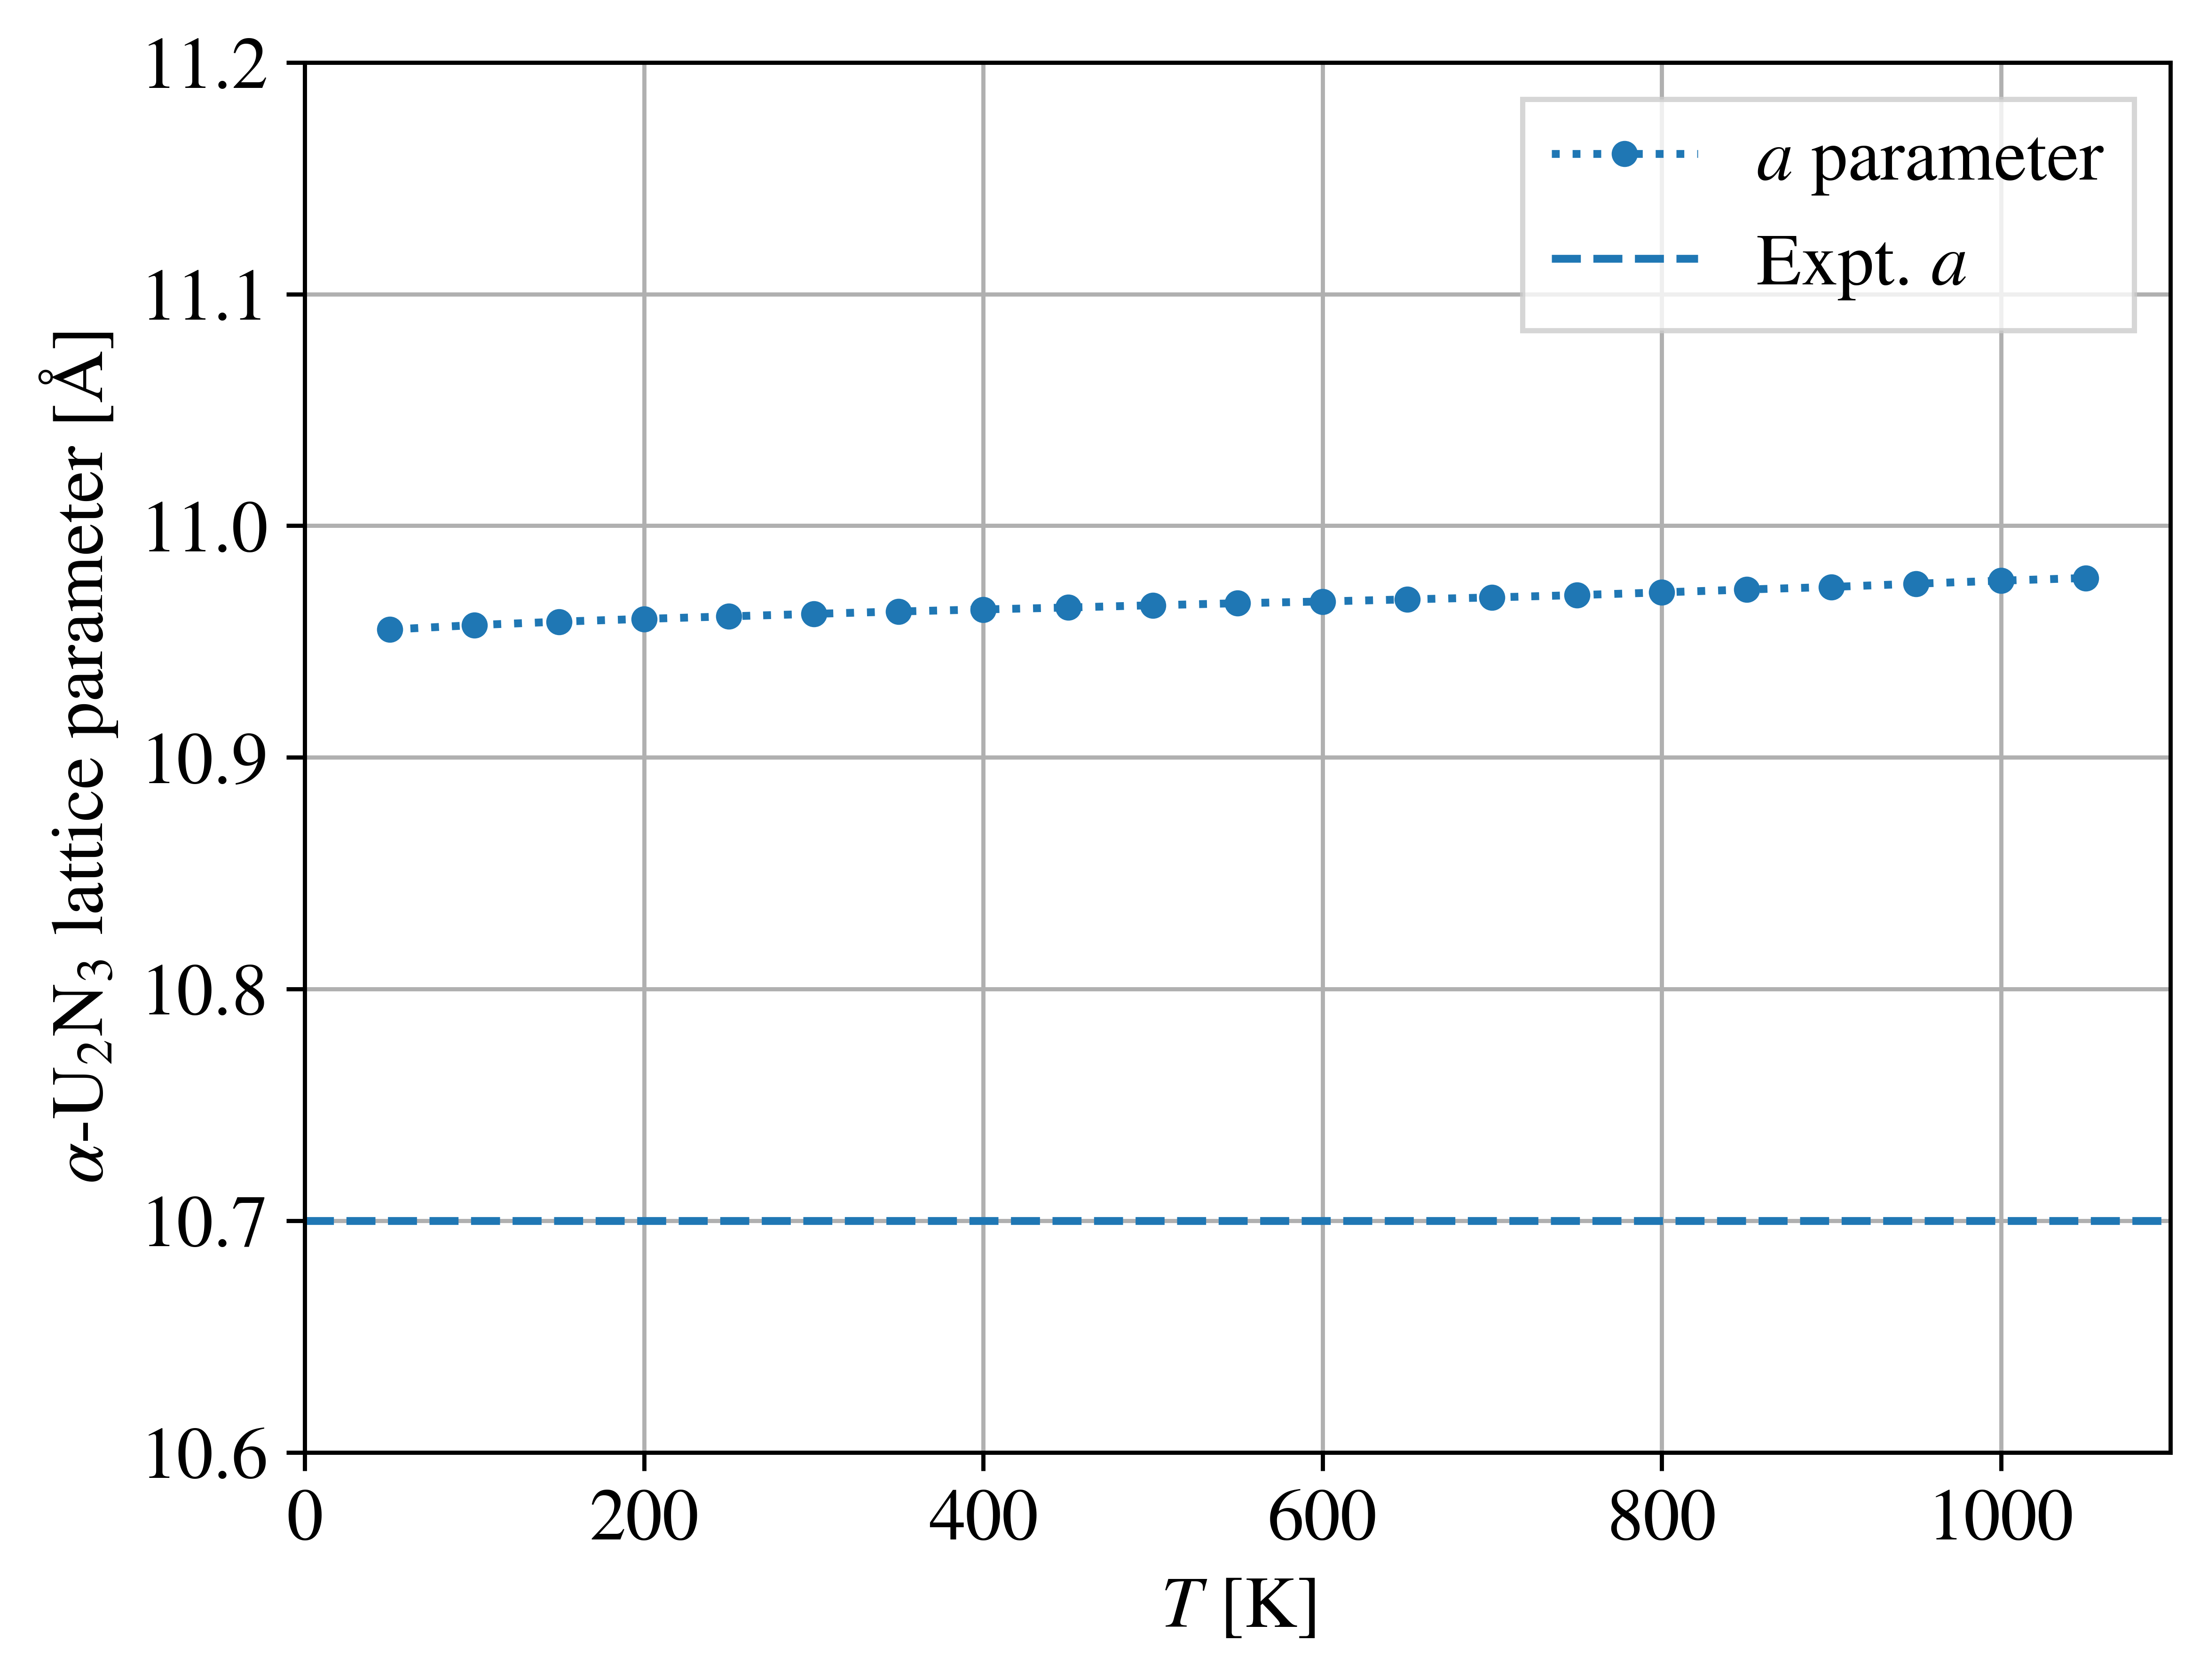
\includegraphics[width=\textwidth]{aU2N3.png}
    \caption{}
    \label{Fig:aU2N3}
\end{subfigure}
\hfill
\begin{subfigure}{0.45\textwidth}
    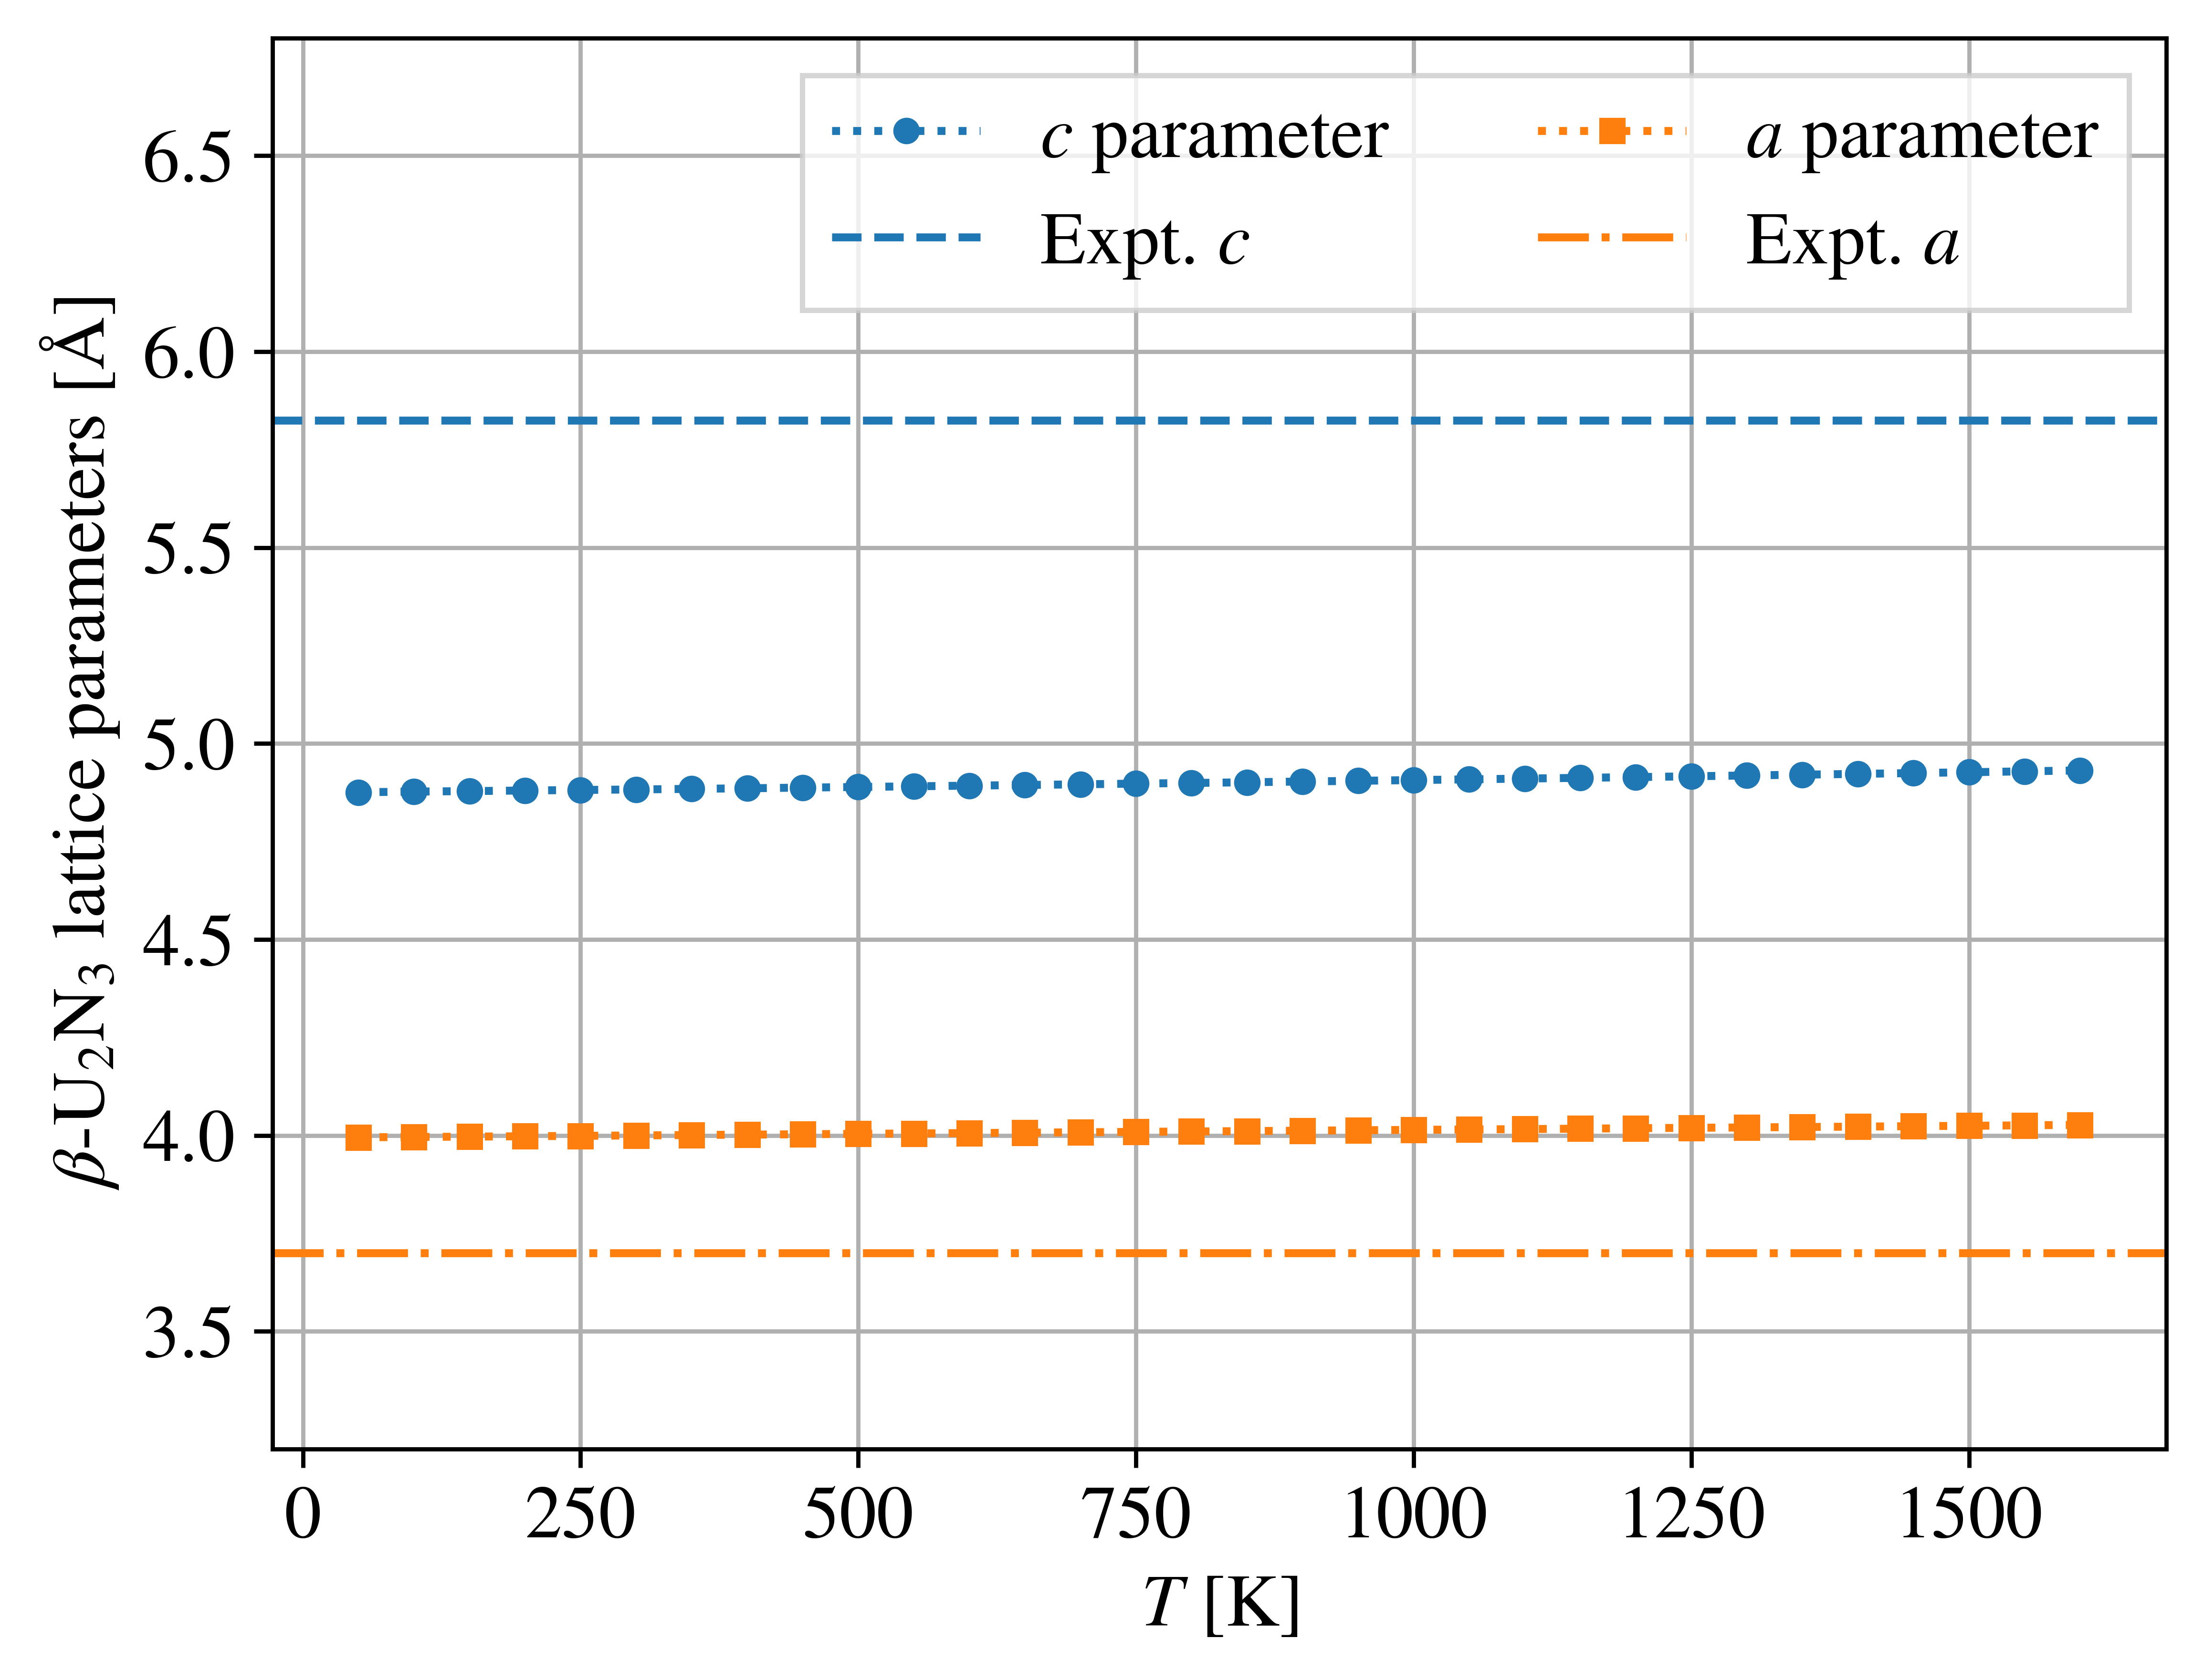
\includegraphics[width=\textwidth]{bU2N3.png}
    \caption{}
    \label{Fig:bU2N3}
\end{subfigure}
\hfill
\begin{subfigure}{0.45\textwidth}
    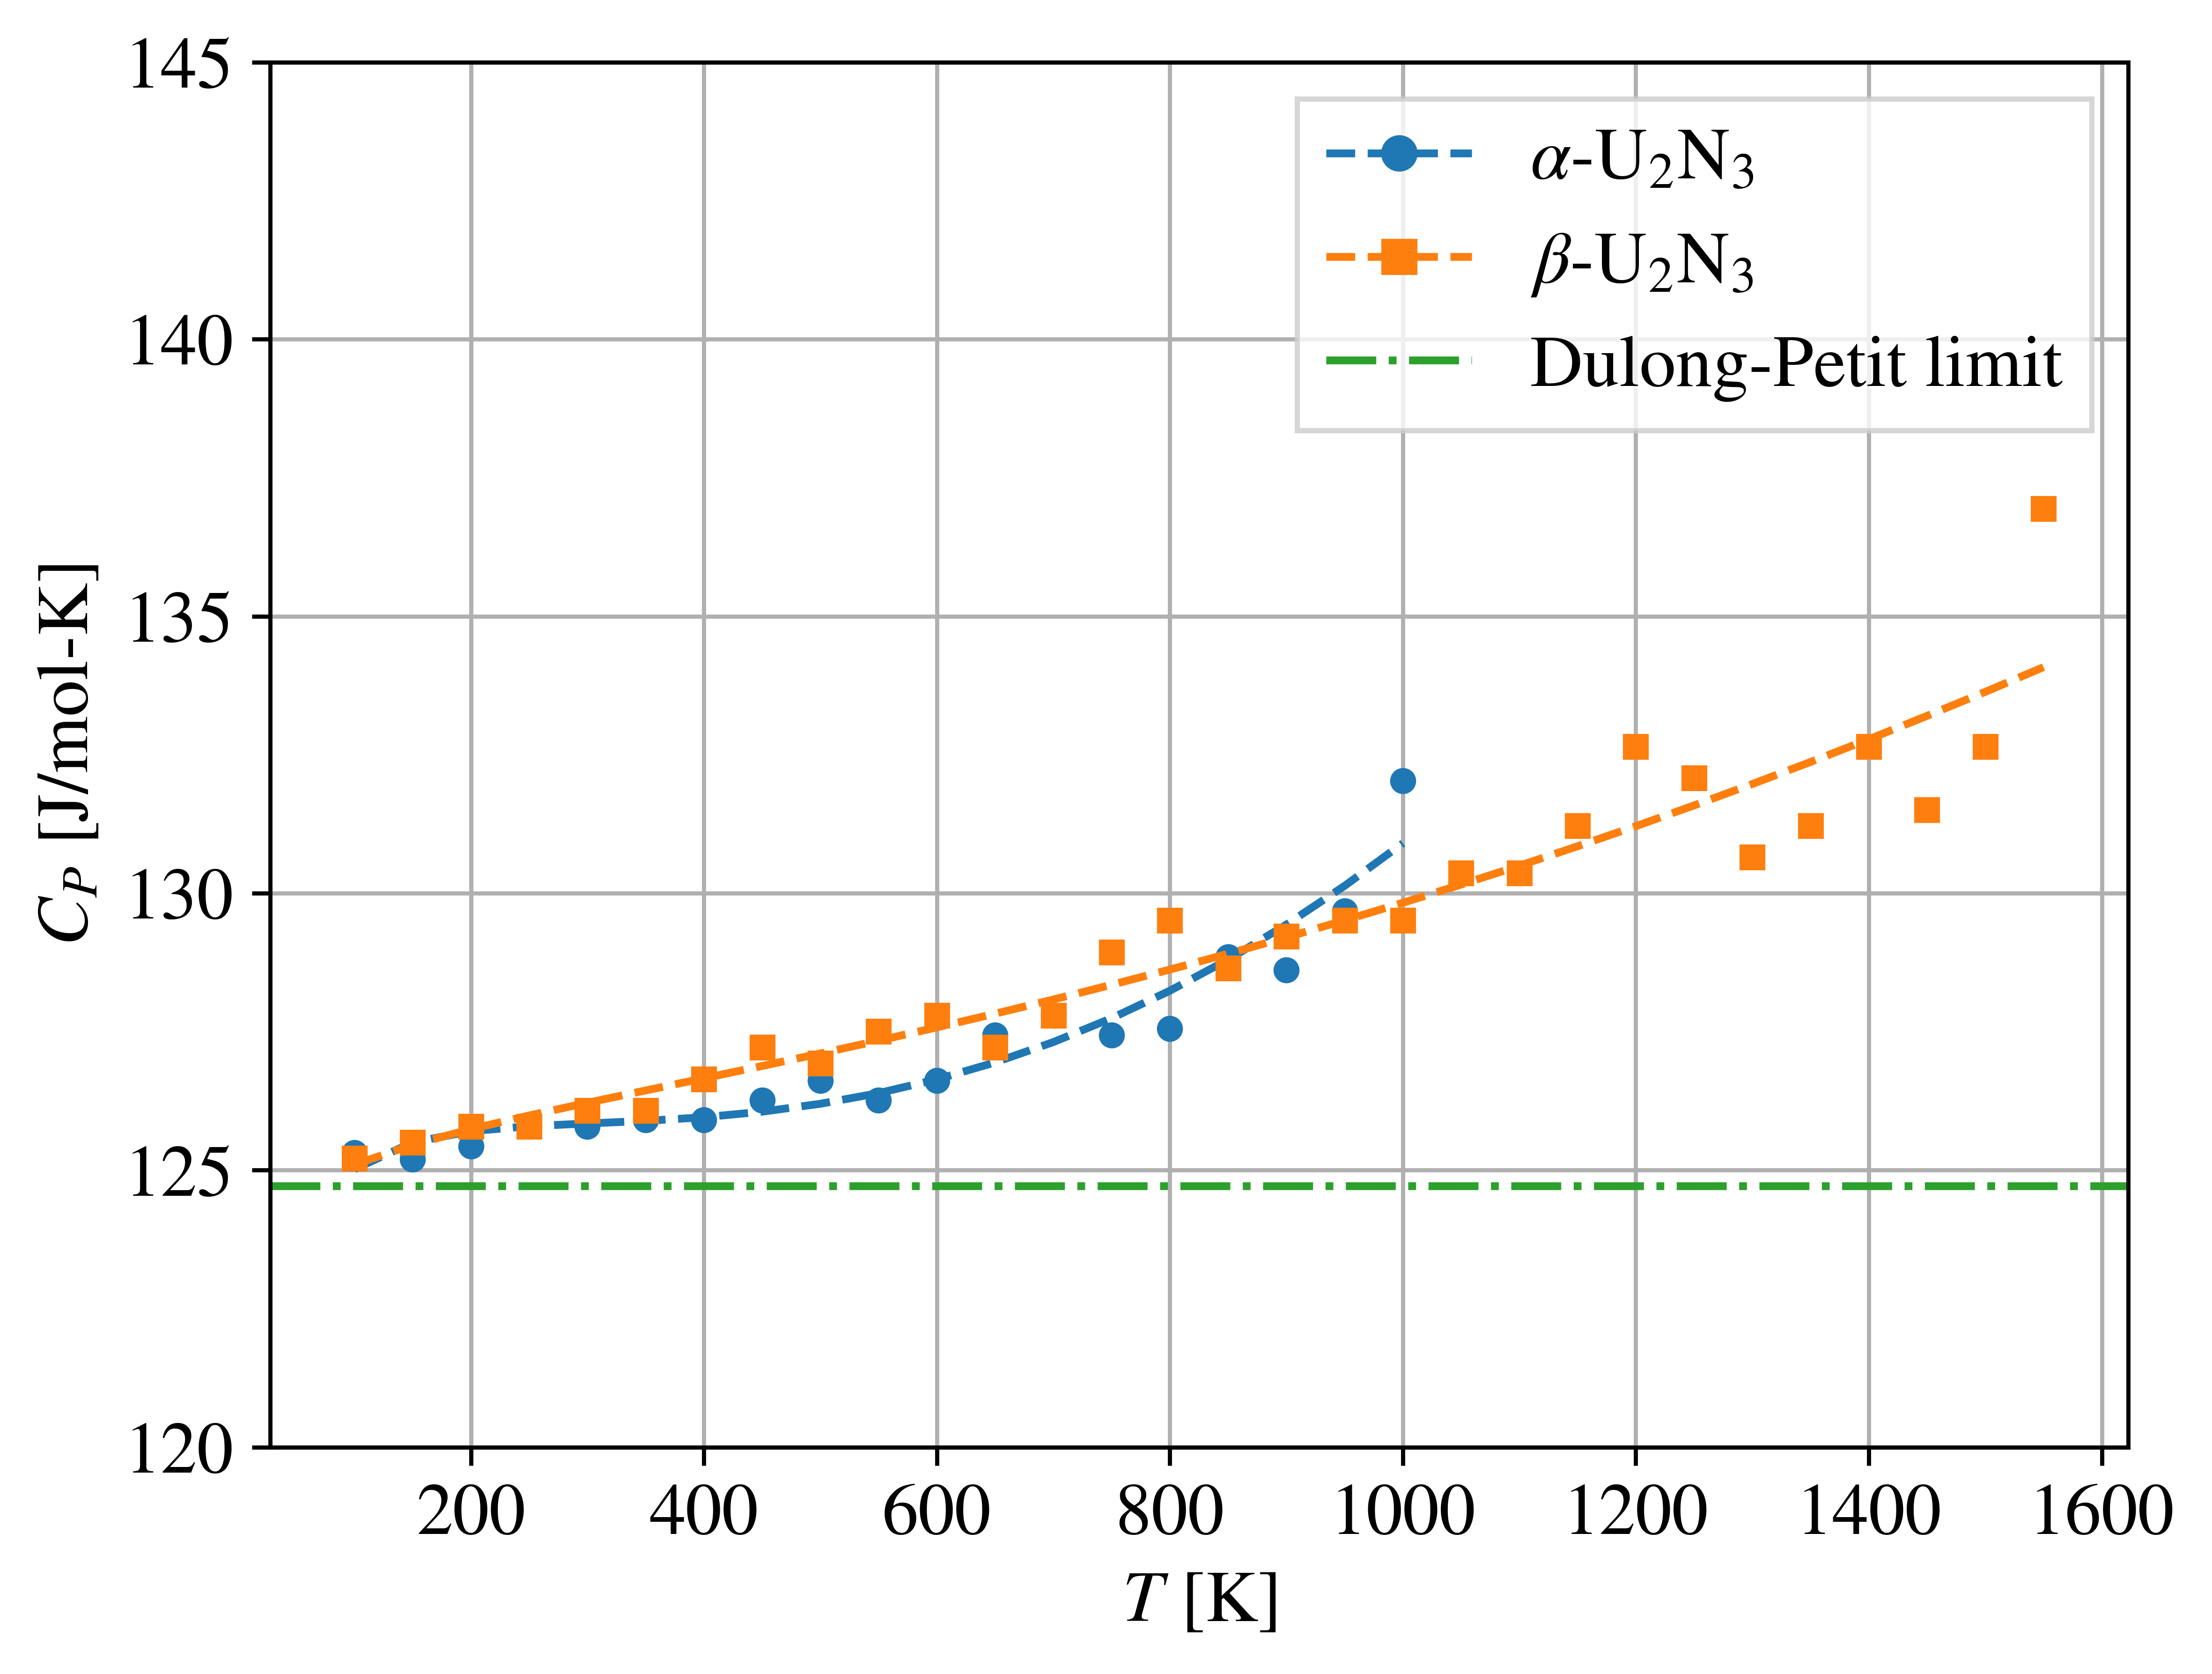
\includegraphics[width=\textwidth]{U2N3CP.png}
    \caption{}
    \label{Fig:U2N3CP}
\end{subfigure}
\caption{The lattice parameters of \textbf{(a)} $\alpha$-\ce{U2N3}, and \textbf{(b)} $\beta$-\ce{U2N3} as calculated by the Kocevski potential. \textbf{(c)} The specific heats of $\alpha$- and $\beta$-\ce{U2N3} as calculated by the Kocevski potential. The curve fit of $C_P$ of $\alpha$- and $\beta$-\ce{U2N3} as functions of temperature are given in \cref{CPU2N3,CPU2N3b}.}
\label{Fig:U2N3}
\end{figure}



\bibliographystyle{elsarticle-num}
\bibliography{ref}

\end{document}